%!TEX root = ../report.tex

\begin{document}
    \chapter{Task 2.0}
    \section{Deliverables 2}
    \begin{itemize}
        \item[] Update your previous week’s report and add a description of the test for a match with a and the computed motion and the actual and expected accuracy and precision. Include appropriate figures, diagrams, and images backing up any claims you make. The report must be self-contained and provide enough details to support any statement you make. If applicable, include a section on problems encountered. Your update should cover:
    \end{itemize}
    
    \begin{itemize}
        \item[1.] Any possible pre-processing of your data, like outlier detection and removal.
        \item[2.] Fit of a Gaussian, either two individual ones in the x and y directions for each of the three cases or a proper two-dimensional distribution per case.
        \item[3.] Check whether the data are actually distributed according to a Gaussian distribution.
        \item[4.] List of used software, including source of any function you wrote for performing your analysis.
        \item[5.] An answer to the following question: When analysing the data with respect to the executed motions, which characteristic of the data do you establish here: the accuracy, the precision, or both?
        \item[6.] For presenting some of the statistical parameters that characterize the observed robot behaviour, in your report, as an example, you can use the structure defined by table 4 (section A.2).
    \end{itemize}
    
    \section{Preprocessing of Data}
    
    {
    \begin{itemize}
        \item Carrying out the experiment in Task 1, we obtained a total of 9 set of measurements -
        \begin{itemize}
            \item X axis coordinates (in cm) for the forward, left and right motions
            \item Y axis coordinates (in cm) for the forward, left and right motions
            \item Theta or the orientation (in degrees) for the forward, left and right motions
        \end{itemize}
        \item \textcolor{red}{Combining the measurements obtained during the experiment in Task 1 from all 6 groups, we got a total of 120 data points in each of the above mentioned sets. 
        \item Of these, in order to use the data from all the groups, we performed some transformations mentioned in section 2.4.}
        \item The first pre-processing step was to remove the outliers. 
        \begin{itemize}
            \item Chebyshev Theorem (Eq 3.1 and 3.2.) was used to remove the outliers. It states that "only a certain amount of data points in a probability distribution can be present from a particular distance from the mean of the distribution".
             \begin{equation}
                P(\mid X - \mu \mid \leq k \sigma) \geq (1 - \frac{1}{k^2})
            \end{equation}
            \begin{equation}
                P(\mid X - \mu \mid \geq k \sigma) \leq \frac{1}{k^2}
            \end{equation}
            \item The number of outliers detected in each set is represented in the Table \ref{tab:outliers}. The code used for this is given below.
            \begin{table}[]
                \centering
                \resizebox{\textwidth}{!}{%
                \begin{tabular}{l l r r}
                \hline
                Motion                   & Random Variable       & Original Data Points & Outlier Count \\ \hline
                \multirow{3}{*}{Forward} & X (cm)                & 120 & 6             \\  
                                         & Y (cm)                &       120               & 3             \\  
                                         & Orientation (degrees) &         120             & 1             \\  
                \multirow{3}{*}{Left}    & X (cm)                &        120              & 0             \\ 
                                         & Y (cm)                &        120              & 1             \\  
                                         & Orientation (degrees) &          120            & 8             \\ 
                \multirow{3}{*}{Right}   & X (cm)                &           120           & 5             \\  
                                         & Y (cm)                &           120           & 2             \\ 
                                         & Orientation (degrees) &           120           & 0            \\ \hline
                \end{tabular}%
                }
                \caption{\textcolor{red}{Outlier Detection}}
                \label{tab:outliers}
            \end{table}
    
            \begin{minted}{python}
    def detect_outliers(data, pp1 = 0.01, pp2 = 0.001) -> (int, np.array([])):
            '''
            Detect outliers based on Chebychev Theorem
            
            Returns
            ---------
            outlier_data_indices:  Indices of outliers detected
            final_data: Filtered data
            '''
            
            outlier_data_indices = []
            
            mu1, sigma1 = mean_variance(data)
            k = 1 / np.sqrt(pp1)
            odv1u = mu1 + k * sigma1
            odv1l = mu1 - k * sigma1
            
            new_data = data[np.where(data <= odv1u)[0]]
            outlier_data_indices.append(list(np.where(data >= odv1u)[0]))
            
            new_data = new_data[np.where(new_data >= odv1l)[0]]
            outlier_data_indices.append(list(np.where(new_data <= odv1l)[0]))
            
            mu2, sigma2 = mean_variance(new_data)
            k = 1 / np.sqrt(pp2)
            odv2u = mu2 + k * sigma2
            odv2l = mu2 - k * sigma2
            final_data = new_data[np.where(new_data <= odv2u)[0]]
            outlier_data_indices.append(list(np.where(final_data >= odv2u)[0]))
            
            final_data = new_data[np.where(final_data >= odv2l)[0]]
            outlier_data_indices.append(list(np.where(final_data <= odv2l)[0]))
            
            return outlier_data_indices, final_data
            \end{minted}
        \end{itemize}
    \end{itemize}
    
    }
    
    \section{Fitting a Gaussian for each measurement}
    \begin{itemize}
        \item The Figures \ref{fig:guassianforwardx}, \ref{fig:guassianforwardy}, \ref{fig:guassianforwardtheta}, \ref{fig:guassianleftx}, \ref{fig:guassianlefty}, \ref{fig:guassianlefttheta}, \ref{fig:guassianrightx}, \ref{fig:guassianrighty} \& \ref{fig:guassianrighttheta} represent the fitting of a Gaussian to the data points after the removal of the outliers.
        \item The table \ref{tab:stats-for-manual-measurements-2} shows the various statistical measures computed for the manually measured data.
        \item Chi square test is performed in order to evaluate how well our data fits to the Gaussian distribution.
        \item The significance level taken for the test is \textcolor{red}{0.05}. It is observed that majority of the data does not fit the \textcolor{blue}{Gaussian} distribution.
        \item The accuracy is computed by comparing the mean value in each set to the true value (from the encoder logs). Further details regarding the accuracy and precision of the measurements are discussed in section 3.6.
        
        \begin{minted}{python} 
    
    def chi_squared_test(data,motion_type,n_bins_observed):
    
    np.random.seed(1)
     
    
    observed_data = data
    
    #Initial bin array and frequncies
    
    bin_array=np.linspace(np.min(observed_data),np.max(observed_data),n_bins_observed)
    

 
    
    ##Make sure there are at least 5 counts in each bin
    bin_check=False
    count=0
    while not bin_check:  
      
        
        observed_freq,_ = np.histogram(observed_data,bin_array)
        
        for index,frequency in enumerate(observed_freq):
            
            
            
            if frequency>=5:
                bin_check=True
                
            else:
                bin_check=False
                ## If its the first bin
                condition1=(index==0)
                
                
                # If its the last bin
                condition2=(index==(len(observed_freq)-1))
                
                if condition1:
                    bin_array=np.delete(bin_array,index+1,axis=0)

                    
                 
                ##If its the last bin
                elif condition2:
                    bin_array=np.delete(bin_array,index,axis=0)

                    
                
                ##If an in between bin
                elif (condition1==False and condition2==False):
                    ##Combine with the adajcent bin with least frequcny 
                 
                    if observed_freq[index-1]<=observed_freq[index+1]:
                        bin_array=np.delete(bin_array,index-1,axis=0)
                        
                    else:
                        bin_array=np.delete(bin_array,index+1,axis=0)
                        
                else :
                    print('Error in bins')
                break                        
                        
  
        
    
    mean = np.mean(observed_data)
    std = np.std(observed_data) 
    expected_data = np.random.normal(mean,std,len(data))  
    expected_freq,_ = np.histogram(expected_data, bin_array)

    dof=np.sum(expected_freq)-1
    
    
    
    #Plot the graph
    x = np.linspace(np.min(observed_data), np.max(observed_data), 100)
    y = scipy.stats.norm.pdf(x, mean, std)    
    fig=plt.figure(figsize=(20,10))
    plt.suptitle(motion_type, size=16)
    ax1=fig.add_subplot(121)
    ax1.hist(expected_data, bin_array, facecolor='blue', alpha=0.5, density=True, edgecolor = 'black')
    ax1.set(title='Expected')
    ax1.grid()
    ax2=fig.add_subplot(122)
    ax2.hist(observed_data, bin_array, facecolor='red', alpha=0.5, density=True, edgecolor = 'black')
    
    ax2.plot(x,y,color='blue')
    ax2.set(title='Observed')
    ax2.grid()
    
    

   

    
    
    chi_value=scipy.stats.chisquare(observed_freq, expected_freq)[0]
    p_value=scipy.stats.chisquare(observed_freq, expected_freq)[1]
    
    
   
    
 
    return (chi_value,p_value)
        \end{minted}
    
    \begin{table}[!ht]
    \centering
    \resizebox{\textwidth}{!}{%
    \begin{tabular}{llrrrrrc}
    \hline
    Motion                   & Random Variable       & Mean  & Variance (cm$^2$) & Accuracy (cm) & Chi Value & P-value & \begin{tabular}[c]{@{}c@{}}Null Hypothesis: Data Fits the Gaussian Distribution\\ (Accept?)\end{tabular} \\ \hline
    \multirow{3}{*}{Forward} & X (cm)                & 0.6       & 1.2         & 0.9           & 8.6     & 0.2     & Suggest to accept                                                                                    \\
                             & Y (cm)                & 46.1       & 0.9           & 0.5           & 5.6     & 0.5     & Suggest to accept                                                                                    \\ 
                             & Orientation (degrees) & -1.0      & 2.0           & 0.9           &  8.0    & 0.2     & Suggest to accept                                                                                   \\ 
    \multirow{3}{*}{Left}    & X (cm)                & -16.1     & 2.8         & 0.5           & 5.6     & 0.2     & Suggest to accept                                                                                    \\ 
                             & Y (cm)                & 35.6      & 0.9           & 0.9           & 10.2    & 0.1     & Suggest to accept                                                                                    \\ 
                             & Orientation (degrees) & 56.2      & 7.6           & 0.3           & 13.6      & 0.0002     & No                                                                                    \\ 
    \multirow{3}{*}{Right}   & X (cm)                & 16.5      & 1.6           & 0.9           & 7.0   & 0.07    & Suggest to accept                                                                               \\ 
                             & {Y (cm)}                & 35.0      & 0.6           & 0.7           &  3.9     & 0.1    & {Suggest to accept}                                                                                    \\ 
                             & Orientation (degrees) & -51.8     & 7.8           & 0.3           &  23.3    & 0.0001     & No                                                                                    \\  \hline
    \end{tabular}%
    }
    \caption{\textcolor{red}{Statistical parameters for manual measurements}}
    \label{tab:stats-for-manual-measurements-2}
    \end{table}

    \end{itemize}
    

    
    \section{Uncertainity Ellipses after PCA}
    
    \begin{itemize}
        \item After removing the outliers, PCA is used to further reduce noise in the data through dimensionality reduction. 
        \item For this, data is projected into k dimensions by using an orthogonal linear transformation. Here, k is represented by the dimensions with the highest variance.
        \item The eigenvectors of the covariance matrix of the data is taken as the target dimensions and they are ranked according to their eigenvalues. Eigenvalues which have the highest values show the highest variance.  
        \item The code snippet used for PCA is given below:
        
           \begin{minted}{python} 
        def get_PCA(data, components = 3):
            X = data
            pca = sklearn.decomposition.PCA(n_components=components)
            pca.fit(X)
            return pca.transform(X)
           \end{minted}
        
        \item Uncertainity ellipses are generally used to depict the pair-wise correlation that exists between any two given  variables. If the correlation between the variables is zero, then the orientation of the error ellipse corresponds to that of the host coordinate system. 
        \item Figures \ref{fig:ellipseforwardafter}, \ref{fig:ellipseleftafter} \& \ref{fig:ellipserightafter} represent the uncertainity ellipses after PCA. After PCA, we see that the components are uncorrelated since we get nearly axis-aligned error ellipses.
    \end{itemize}
    
    
    \section{List of software used}
    \begin{itemize}
        \item All pre-processing and visualisation of of data was carried out using Python. The following libraries were used:
        \begin{itemize}
            \item[1.] numpy
            \item[2.] pandas
            \item[3.] scipy.stats
            \item[4.] matplotlib
            \item[5.] sklearn
        \end{itemize}
    \end{itemize}
    
    \section{Observations regarding manual measurements and encoder logs}
    
    During the process of visualising the evaluated data, we quickly discovered that the encoded data from the EV3 and the measured data did not fit together as good as we would have hoped. For each of the three movement cases we noticed mainly two modes in the data delivered by the encoder -
    
    \begin{itemize}
        \item[1.] The encoder delivers data, which fits to the manually measured measurements.
    
    \end{itemize}
    
    \begin{center}
        OR
    \end{center}
        
    \begin{itemize}
        \item[2.] The encoder delivers data which is way off, the mean of the data points hover around 166 \textcolor{blue}{cm} for both x and y axis.
    \end{itemize}
    
    \textcolor{blue}{We can compare standard error between the two different contributions:}
    
     \begin{itemize}
        \item[1.] Forward case: the standard error is much smaller along the x-axis (encoded: 4.9 \textcolor{blue}{cm}, measured: 31 \textcolor{blue}{cm}). Along the y-axis, the standard error is the same (around 28 \textcolor{blue}{cm} for both)
        \item[2.] Left case: The error along the x-axis is the same for  both methods (24 \textcolor{blue}{cm}), along the y-axis the error is smaller (encoded 17 \textcolor{blue}{cm}, measured 25 \textcolor{blue}{cm})
        \item[3.] Right case: Along the x-axis the encoded has an error  of 38 \textcolor{blue}{cm} and measured around 42 \textcolor{blue}{cm}. Along the y-axis its 24  \textcolor{blue}{cm} and 29 \textcolor{blue}{cm}.
    \end{itemize}
    
    \subsection{Final Thoughts}
    \begin{itemize}
        \item[] \textcolor{ForestGreen}{\textbf{An answer to the following question: When analysing the data with respect to the executed motions, which characteristic of the data do you establish here: the accuracy, the precision, or both?}}
        \item[1.] Since the measured data and encoded data are so far apart, we would rather look at how they are distributed by themselves than together. The raw data points are shown in Figures \ref{fig:encoder-1}, \ref{fig:encoder-2} and \ref{fig:encoder-3}
        \item[2.] Hence it does not make much sense to look at the accuracy of measurements but rather at the precision - which takes into account the error associated with each measurement. For this, refer Figures \ref{fig:encoder-4}, \ref{fig:encoder-5}, \ref{fig:encoder-6} \& \ref{fig:encoder-7} which represent the error ellipses for encoder data vs manually measured data.
        \item[3.] Even after outlier removal from the encoder data, we see a mismatch between the two sets of measurements.
        \item[4.] From the figures \ref{fig:encoder-4}, \ref{fig:encoder-5}, \ref{fig:encoder-6} \& \ref{fig:encoder-7}, it is clear that the measurements from the encoder data are more precise as they have smaller error ellipses. However, the standard deviation of the manually measured data is much higher resulting in larger ellipses and therefore we conclude that the manual measurements are less precise. 
        
        \item[] The data collection of the EV3 fails to provide data in meaningful ways. On the one hand, the data collection is unreliable, which means it randomly fails to deliver correlating to the true movements at all and on the other hand, even if the data is close to the true measurements, the distributions are completely different, see Figure \ref{fig:encoder-7}.
    \end{itemize}
    
         %000000000000000000000000000000000000000000000000000000000000000000000000000000000000%
    
    \begin{figure*}[ht!]
    \centering
       \subfloat[X-axis coordinates \label{fig:guassianforwardx}]{%
          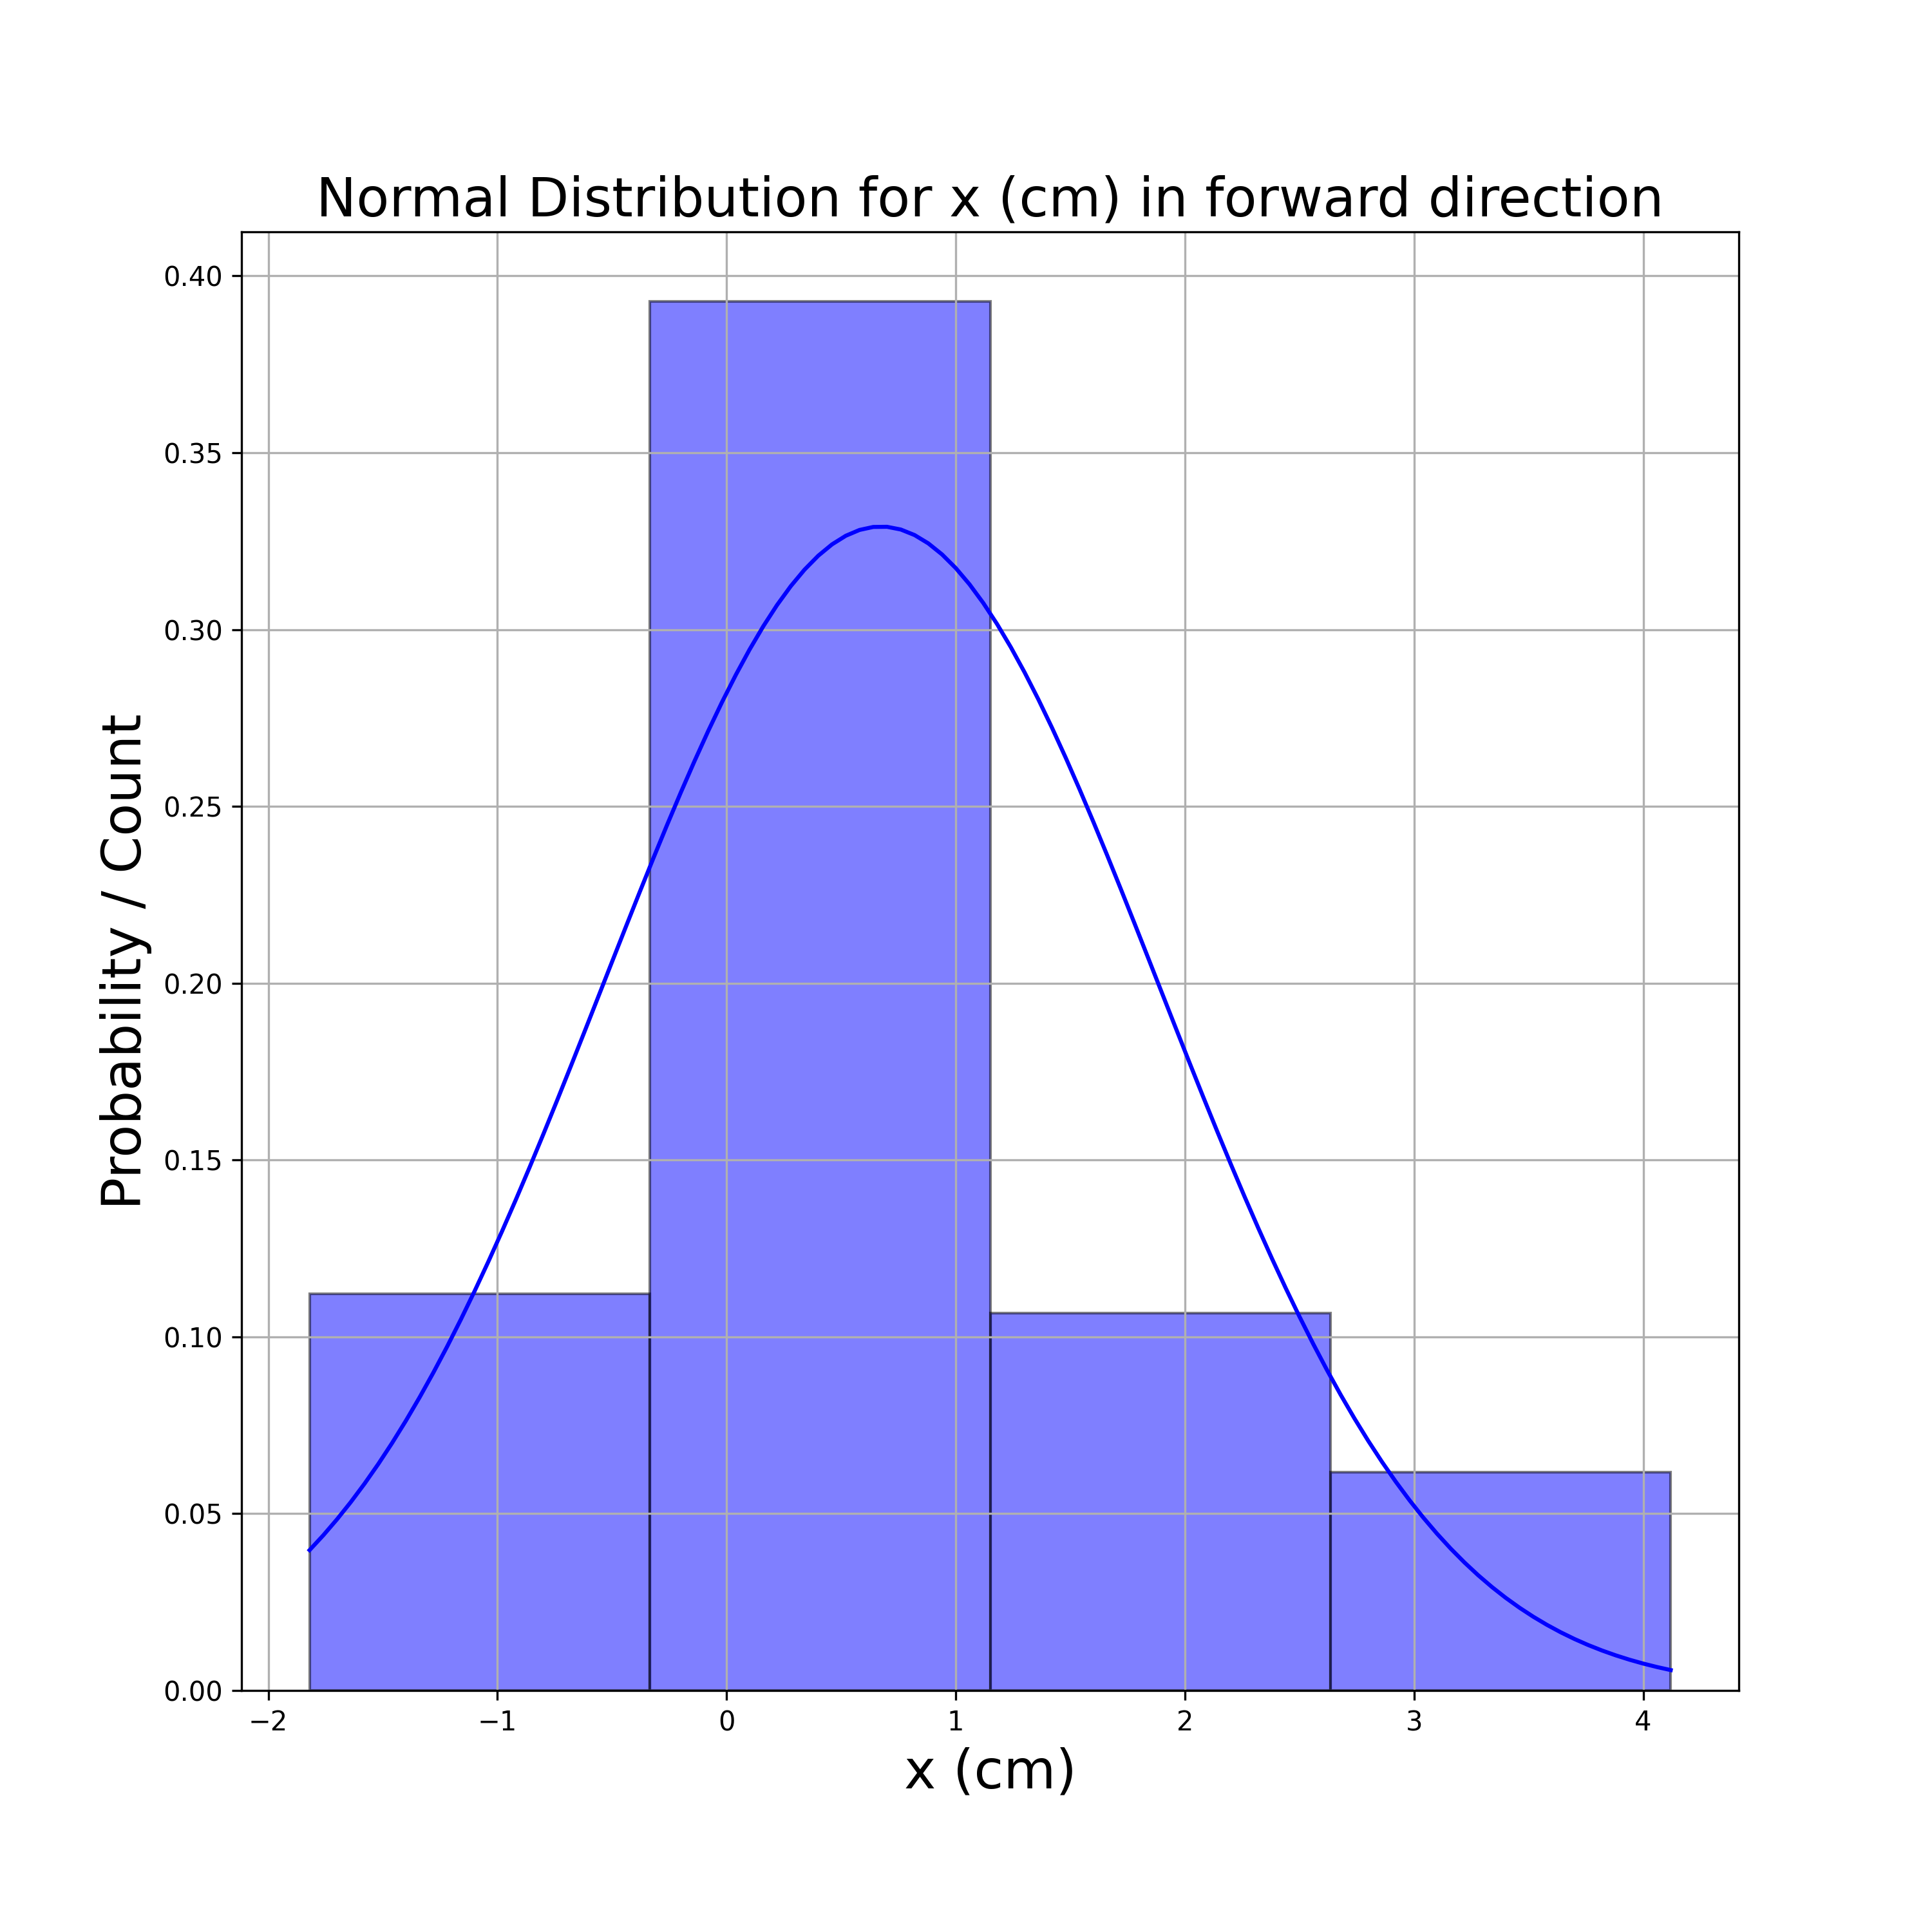
\includegraphics[ width=0.45\textwidth]{"images/experiment_3/normal_distribution_forward_x (cm).png"}}
    \hspace{\fill}
       \subfloat[Y-axis coordinates \label{fig:guassianforwardy} ]{%
          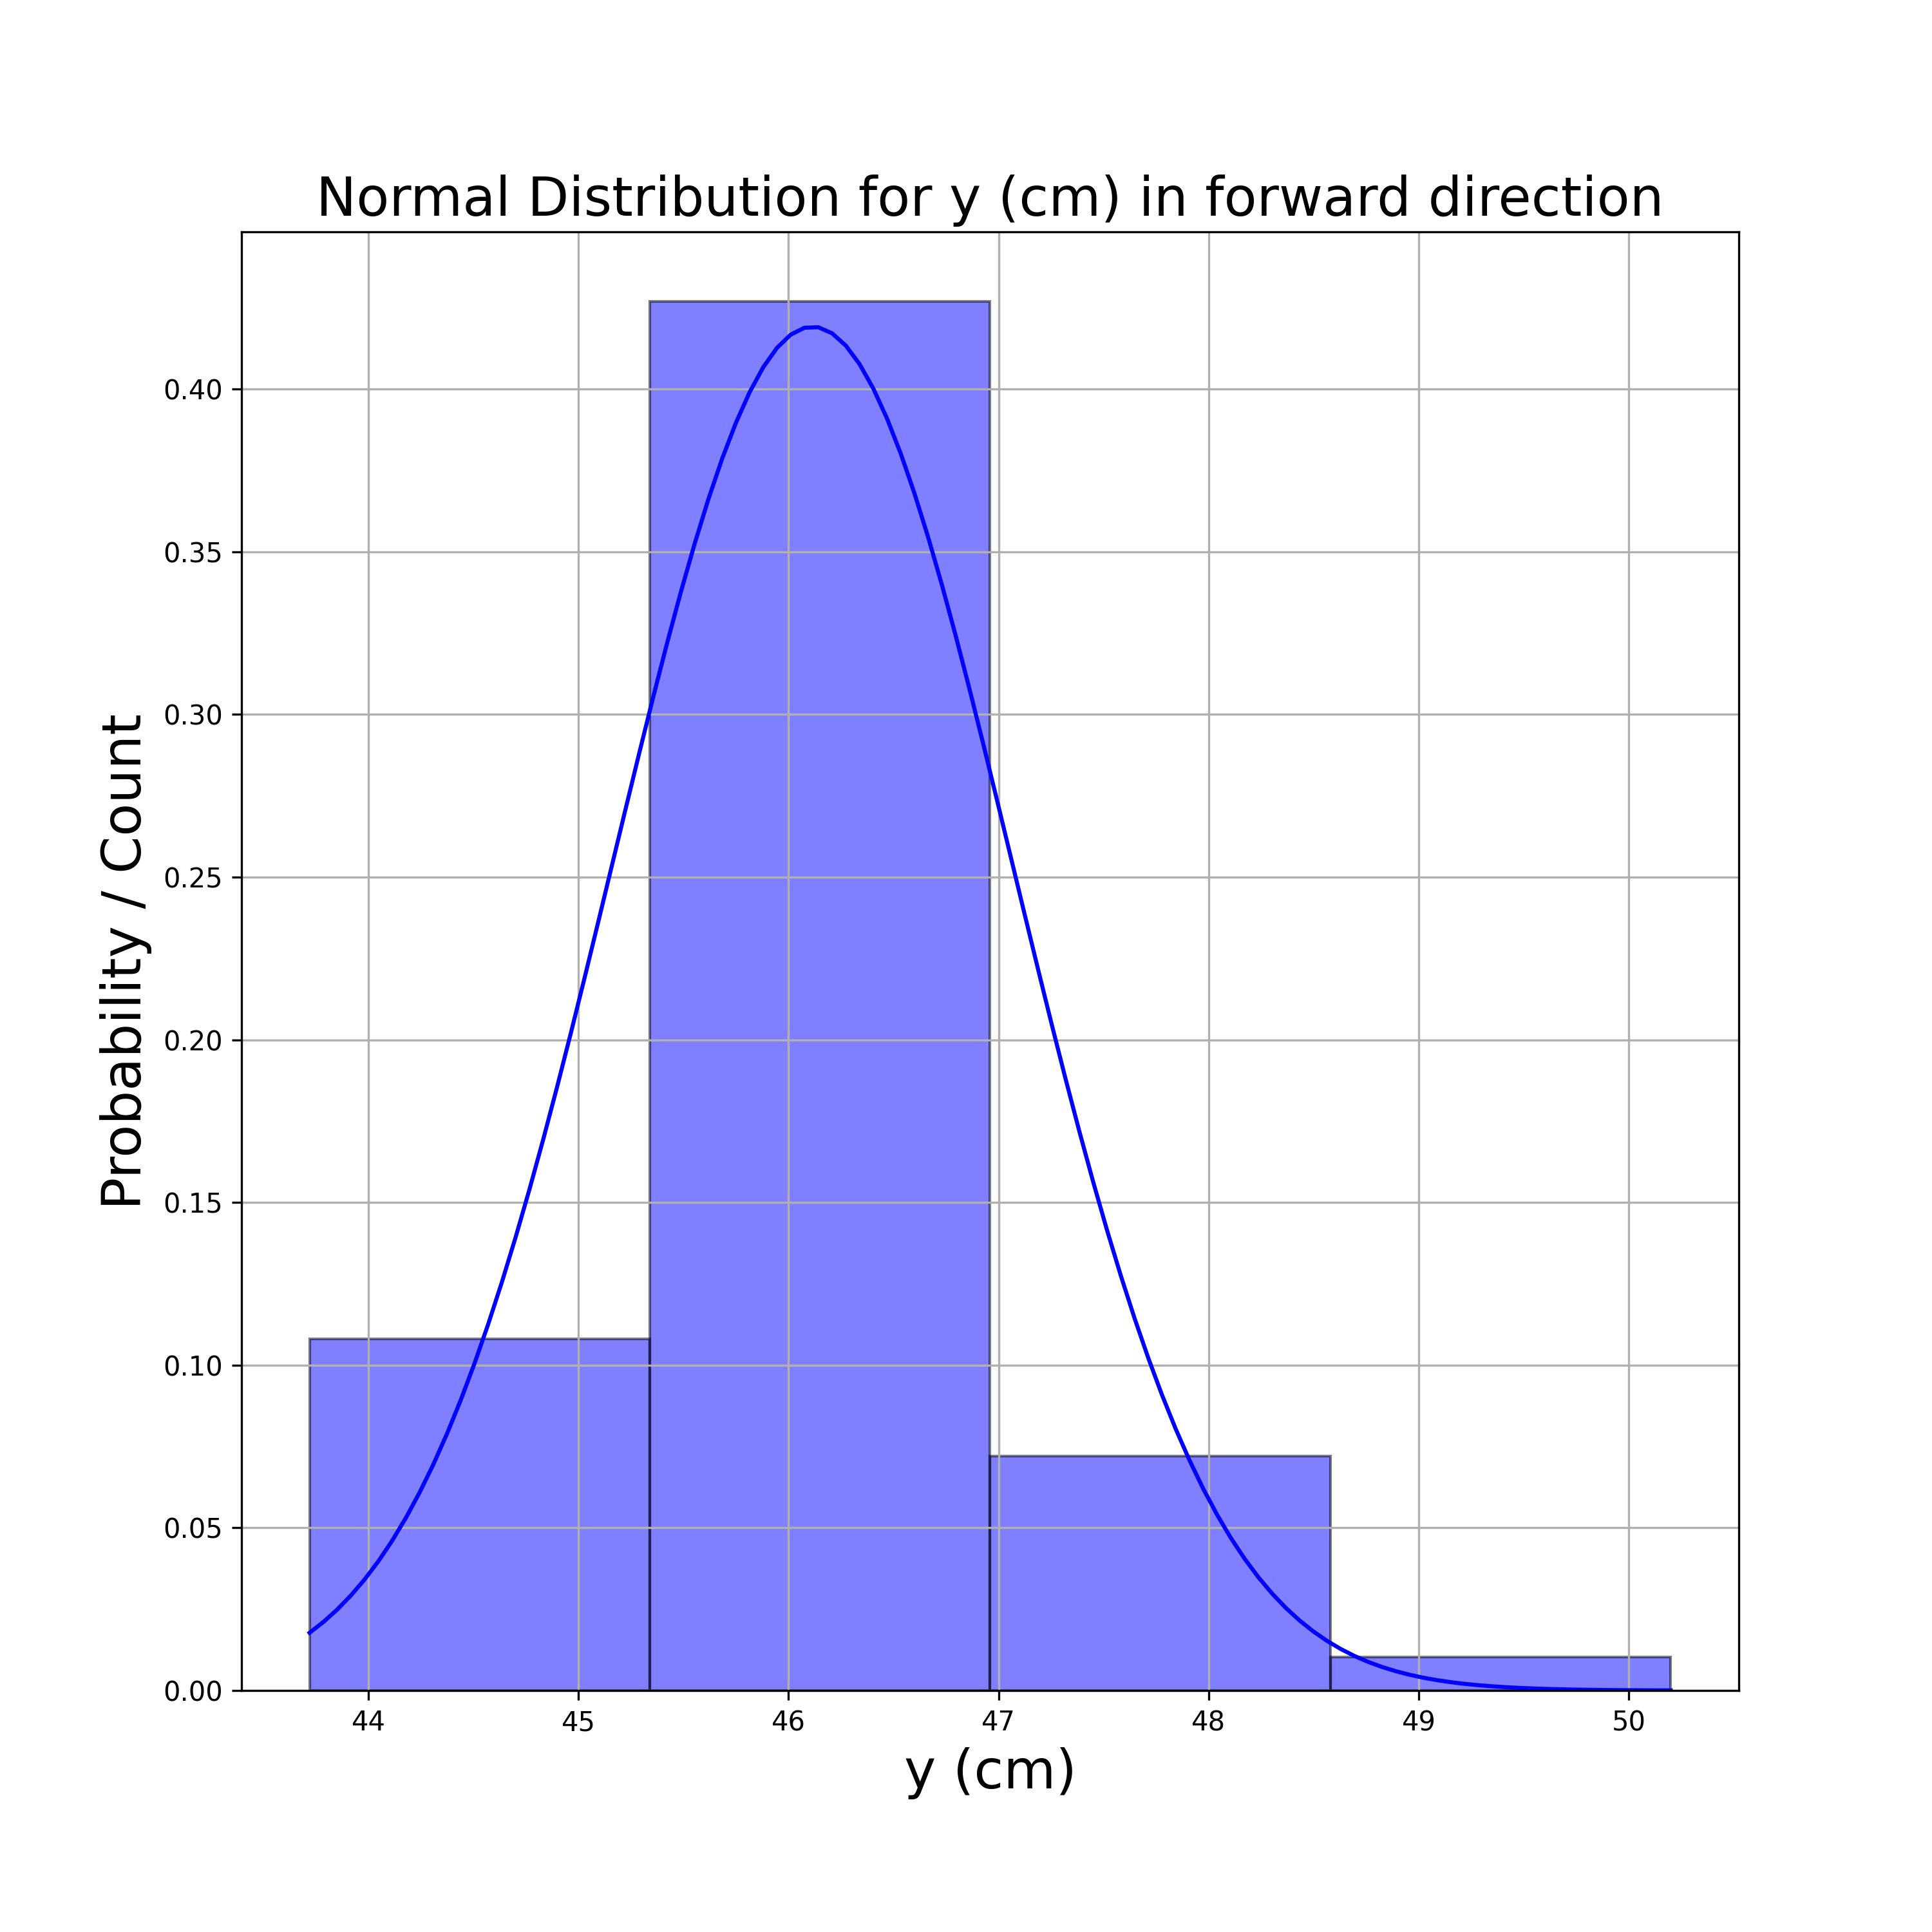
\includegraphics[ width=0.45\textwidth]{"images/experiment_3/normal_distribution_forward_y (cm).png"}}
    \hspace{\fill}
       \subfloat[Orientation \label{fig:guassianforwardtheta}]{%
          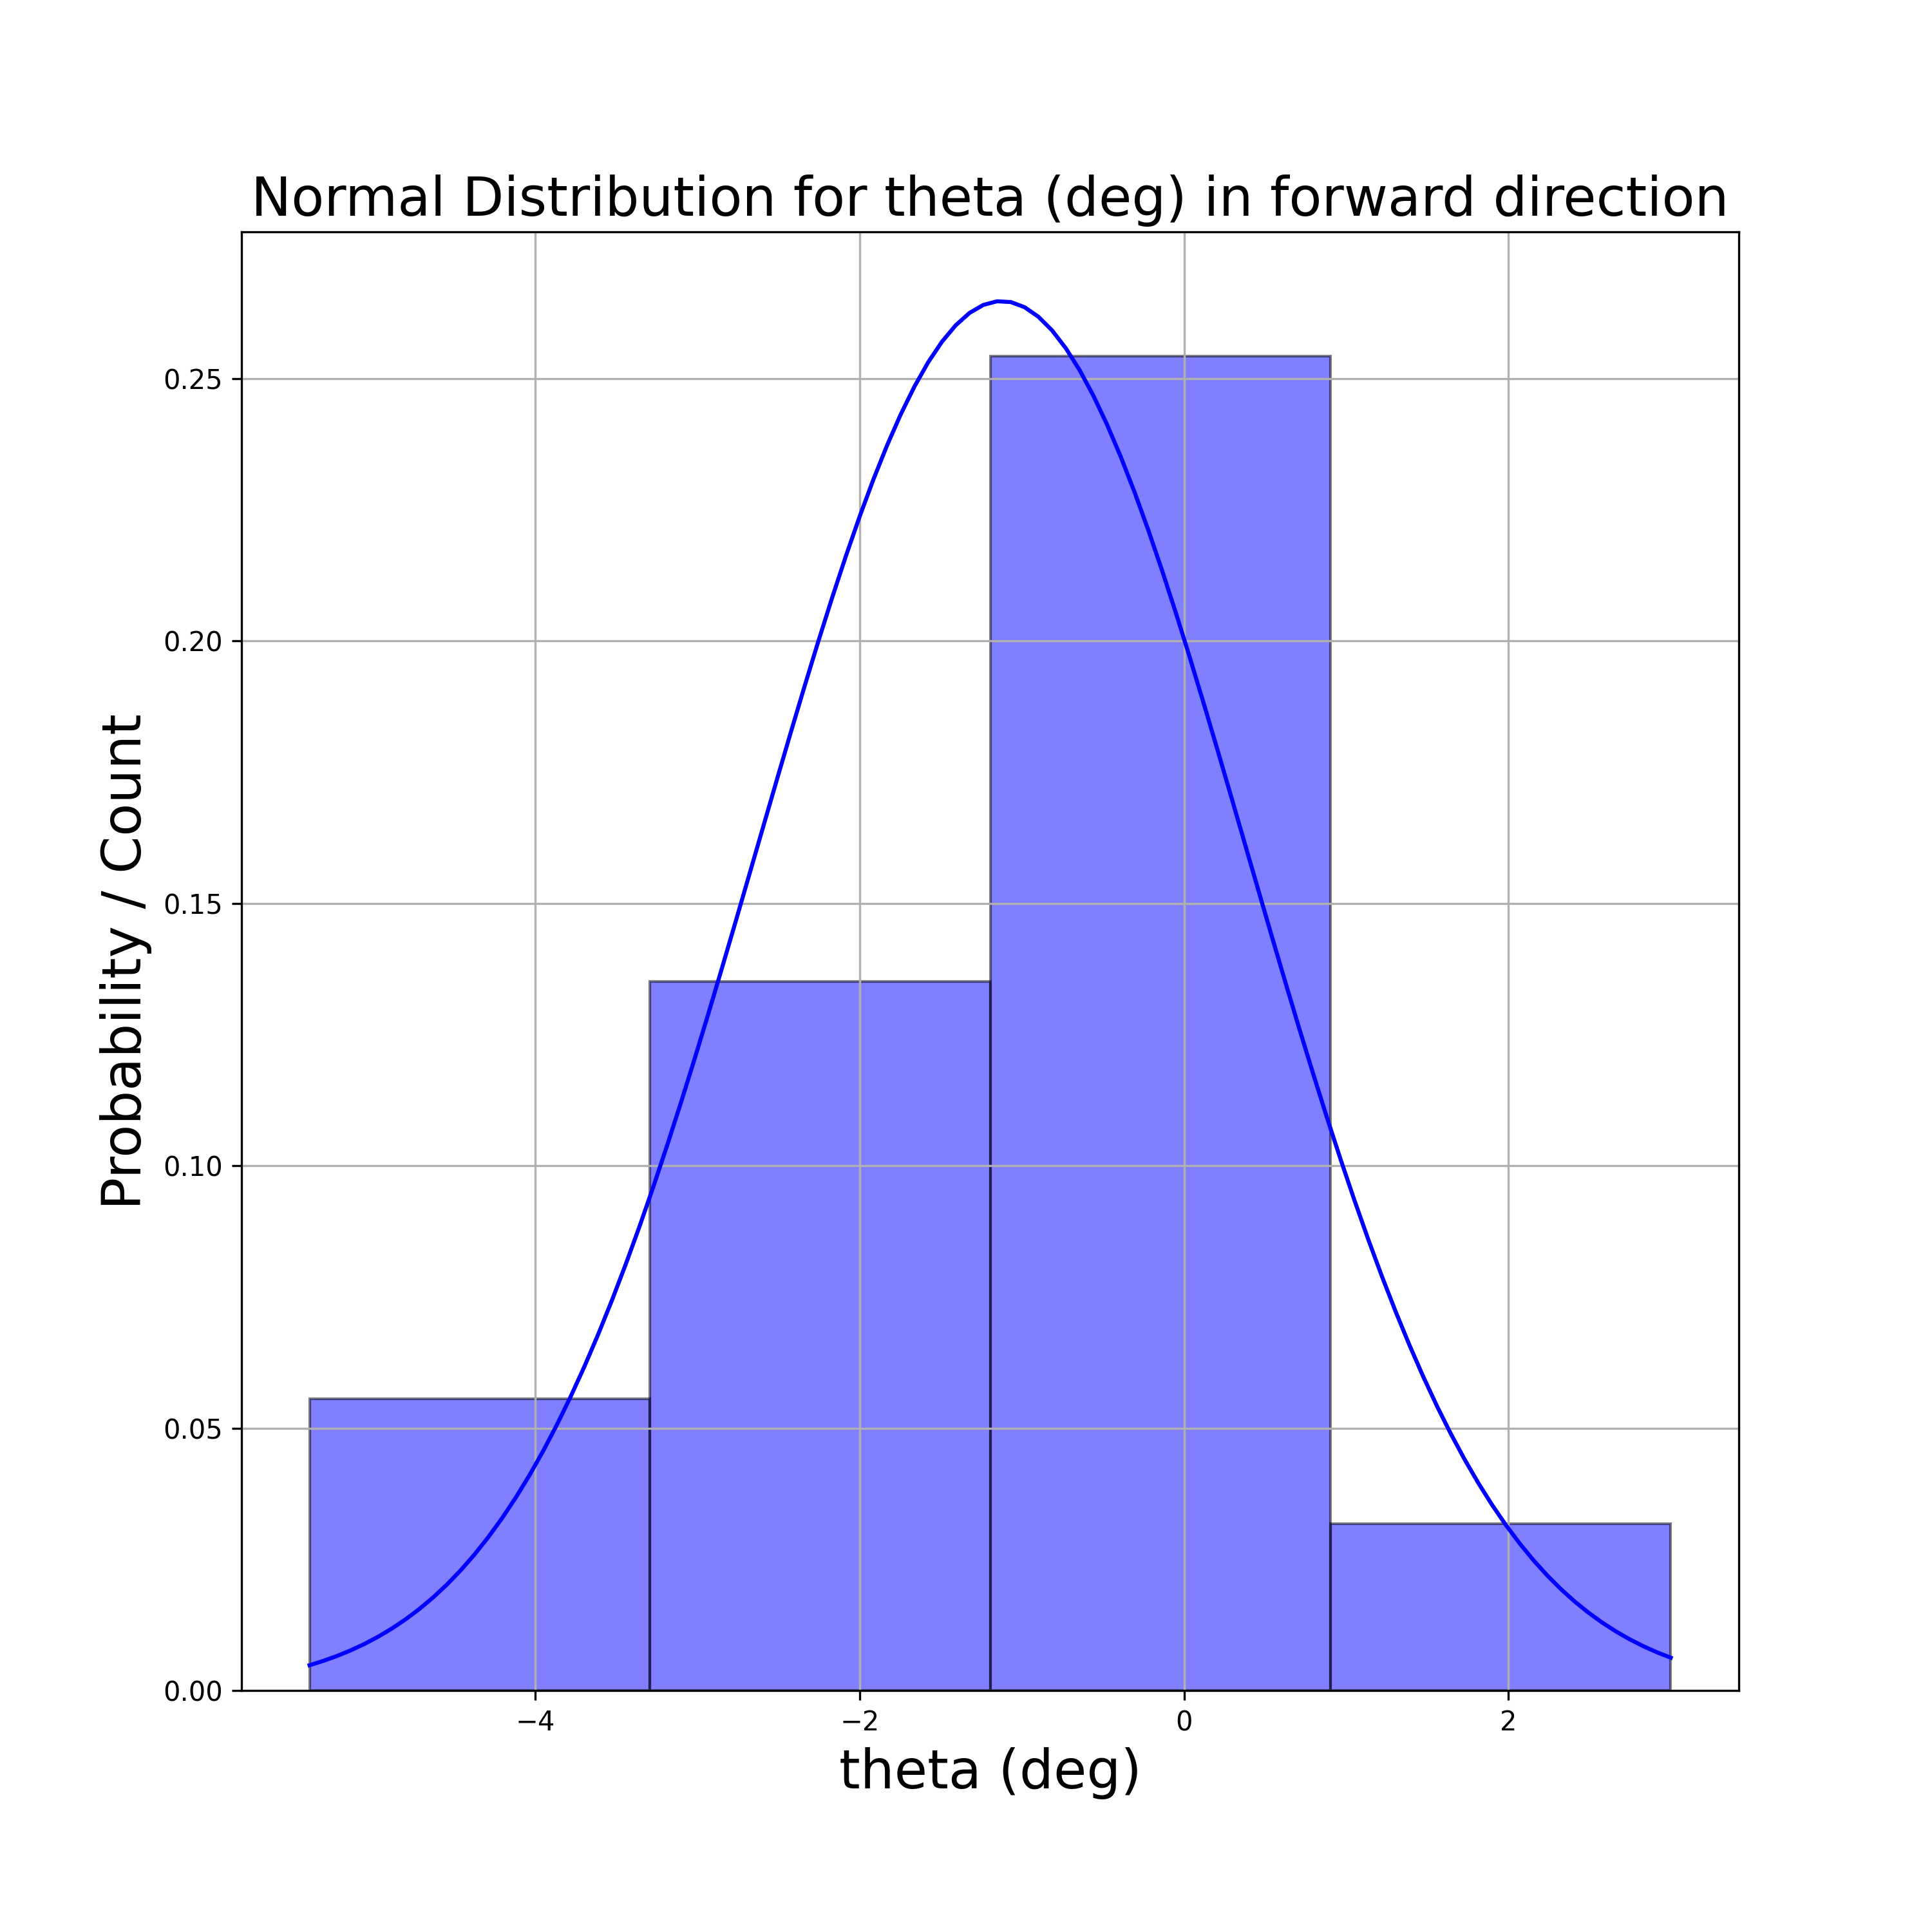
\includegraphics[ width=0.45\textwidth]{"images/experiment_3/normal_distribution_forward_theta (deg).png"}}\\
    \caption{\textcolor{red}{Manually measured x, y and orientation in the forward direction}}
        \label{guassianforward}
    \end{figure*}
    
    %000000000000000000000000000000000000000000000000000000000000000000000000000000000000%
    
    %000000000000000000000000000000000000000000000000000000000000000000000000000000000000%
    \begin{figure*}[ht!]
        \centering
       \subfloat[X-axis coordinates  \label{fig:guassianleftx}]{%
          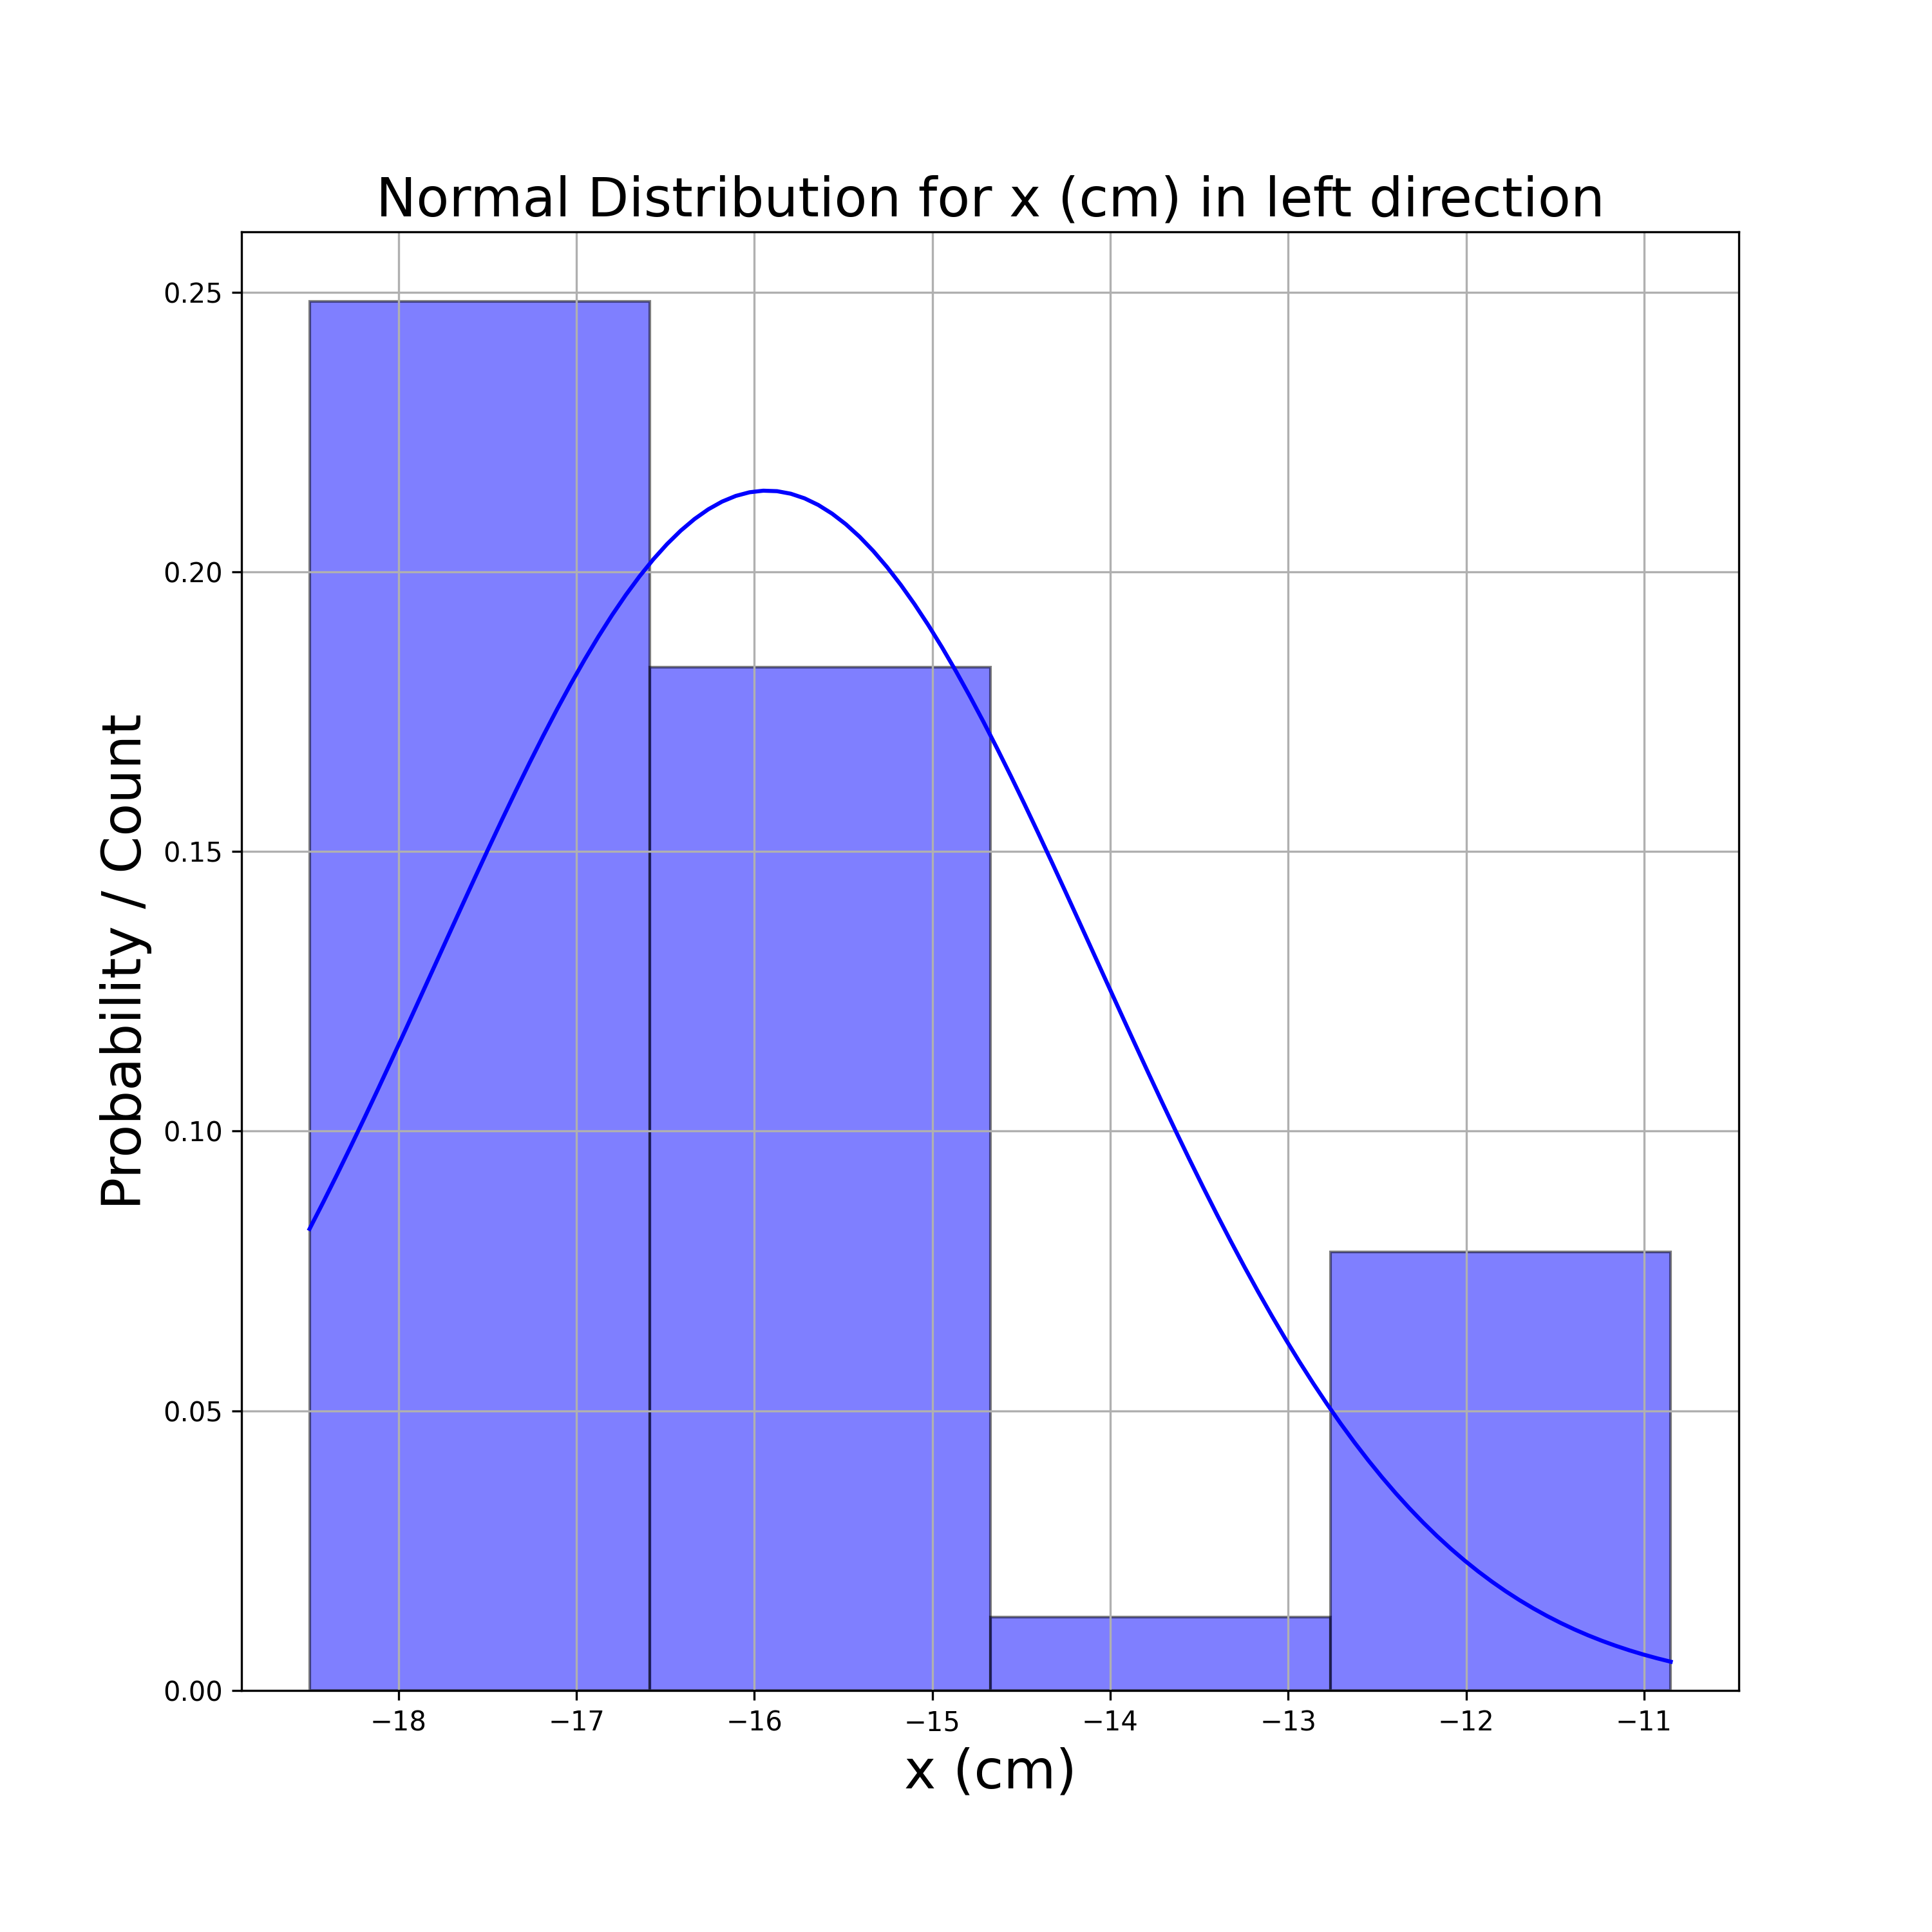
\includegraphics[ width=0.45\textwidth]{"images/experiment_3/normal_distribution_left_x (cm).png"}}
    \hspace{\fill}
       \subfloat[Y-axis coordinates  \label{fig:guassianlefty} ]{%
          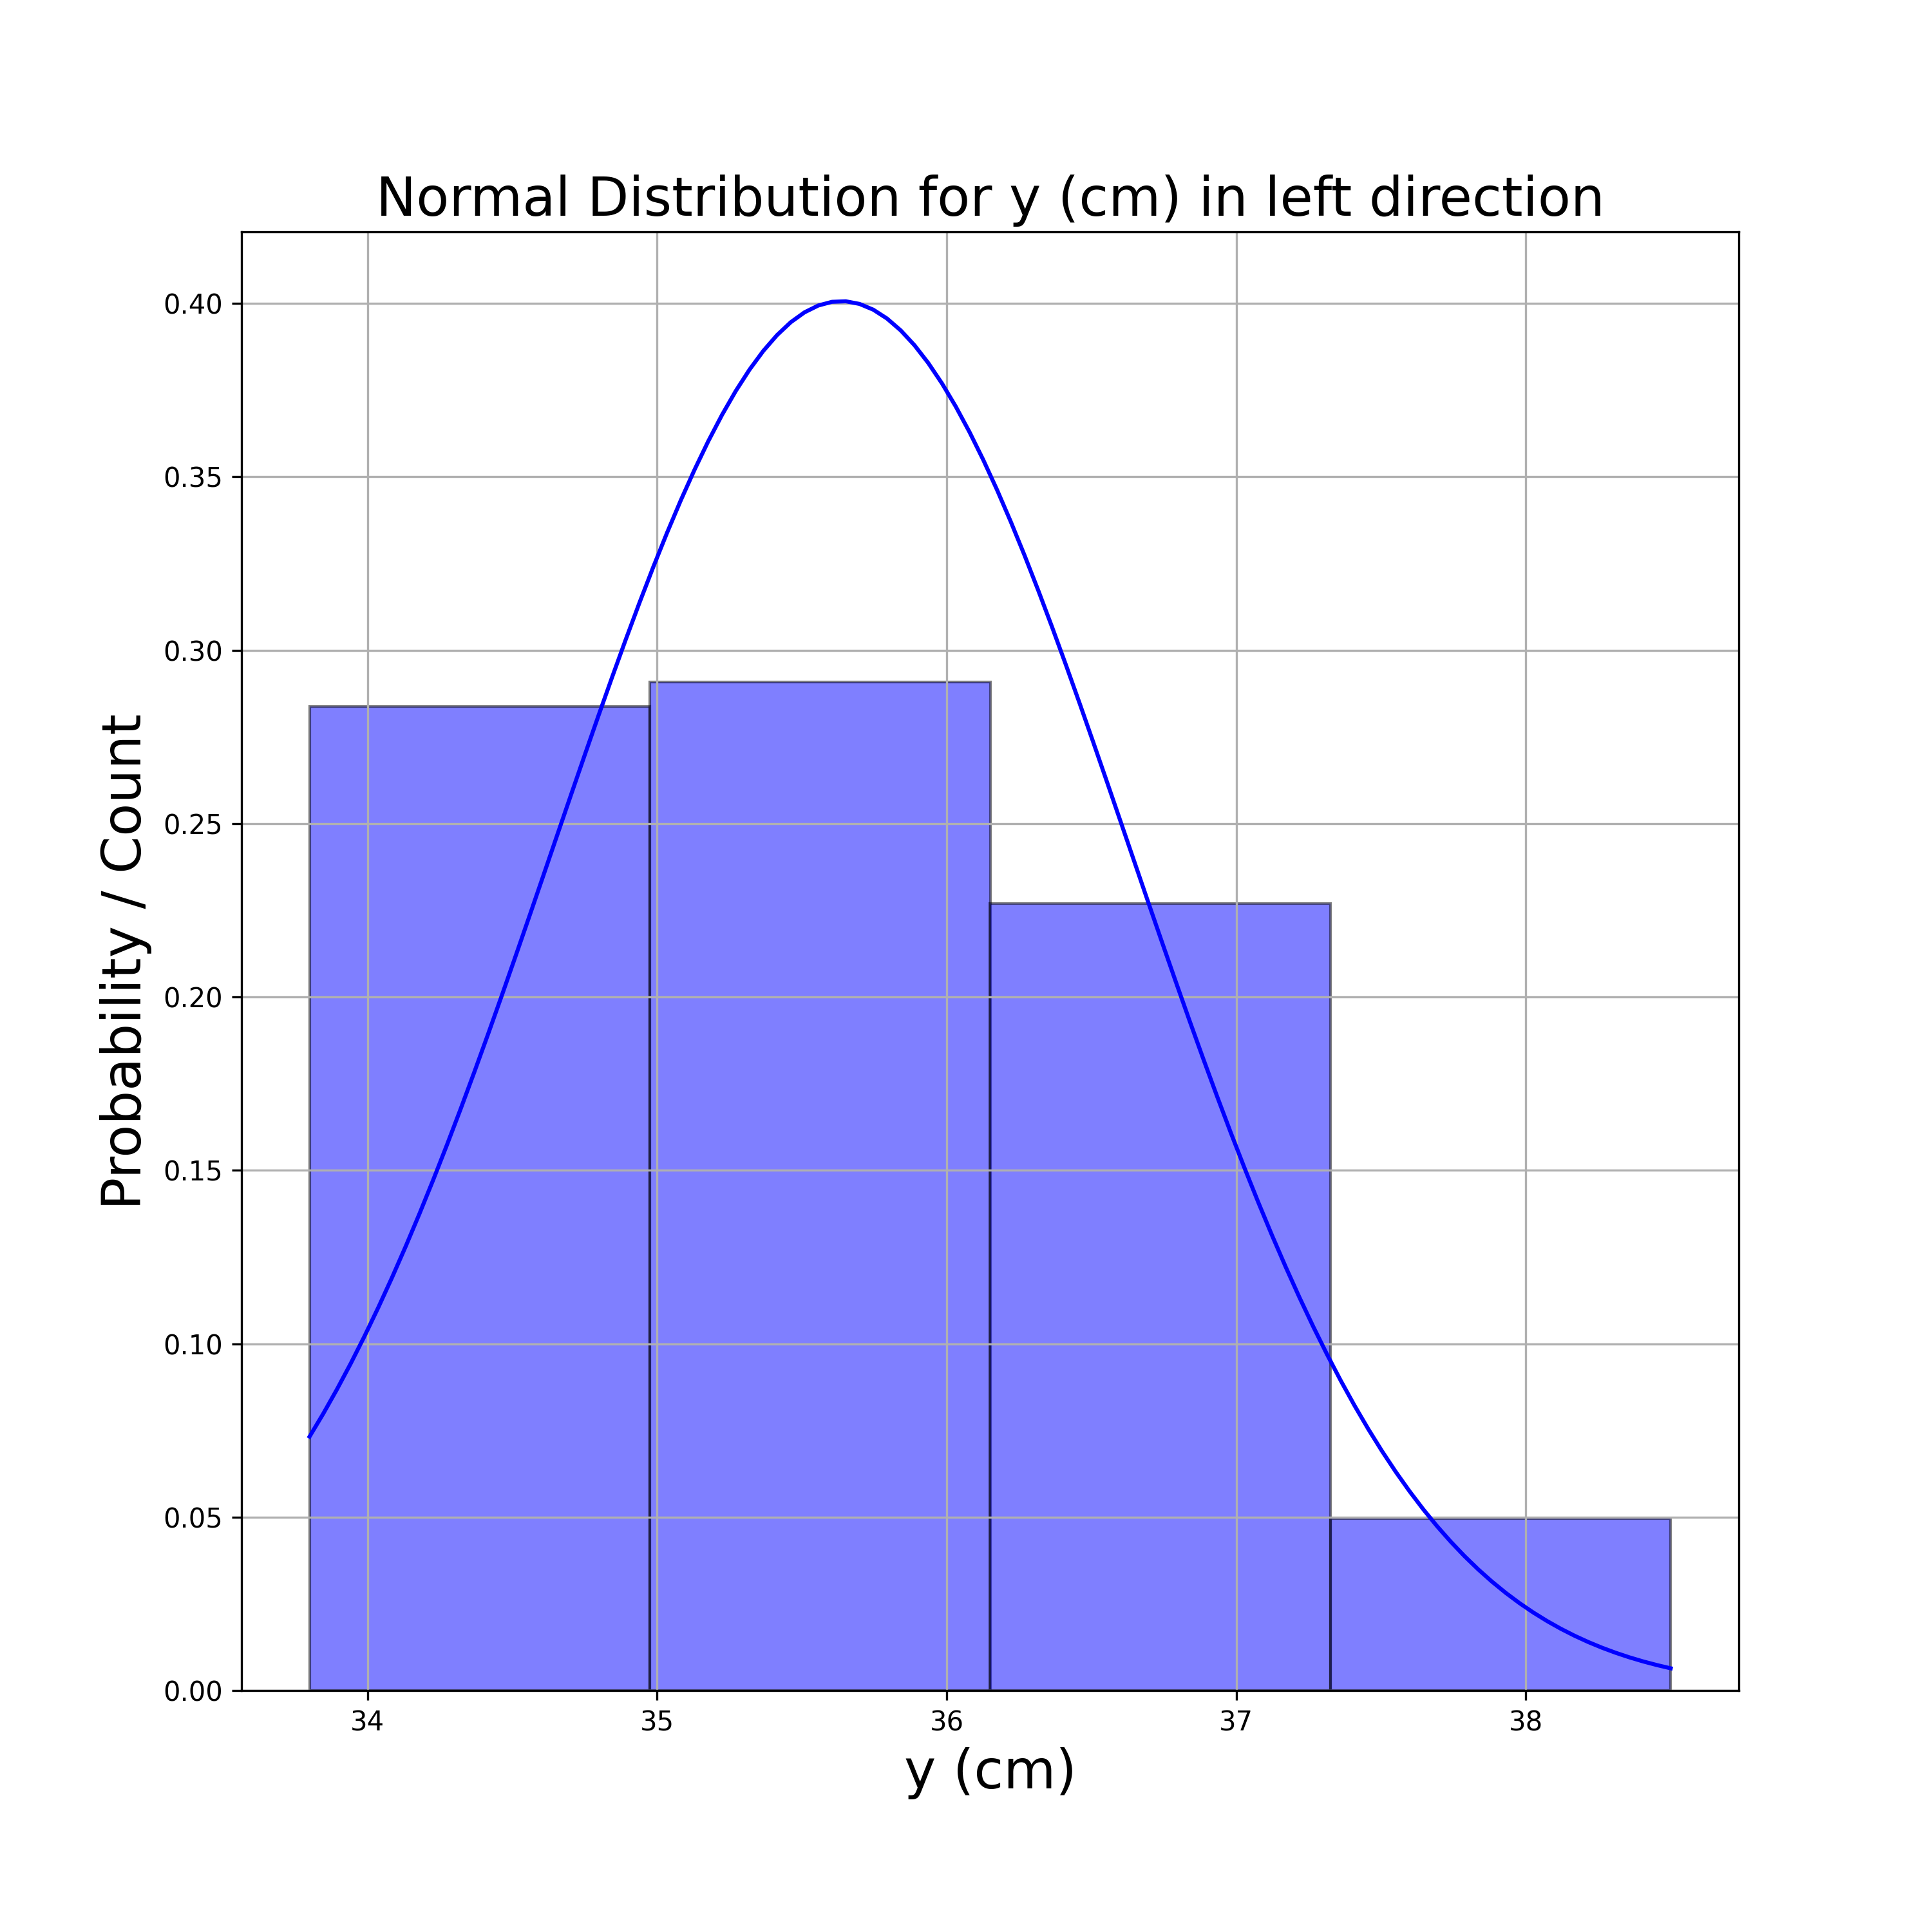
\includegraphics[ width=0.45\textwidth]{"images/experiment_3/normal_distribution_left_y (cm).png"}}
    \hspace{\fill}
       \subfloat[Orientation \label{fig:guassianlefttheta}]{%
          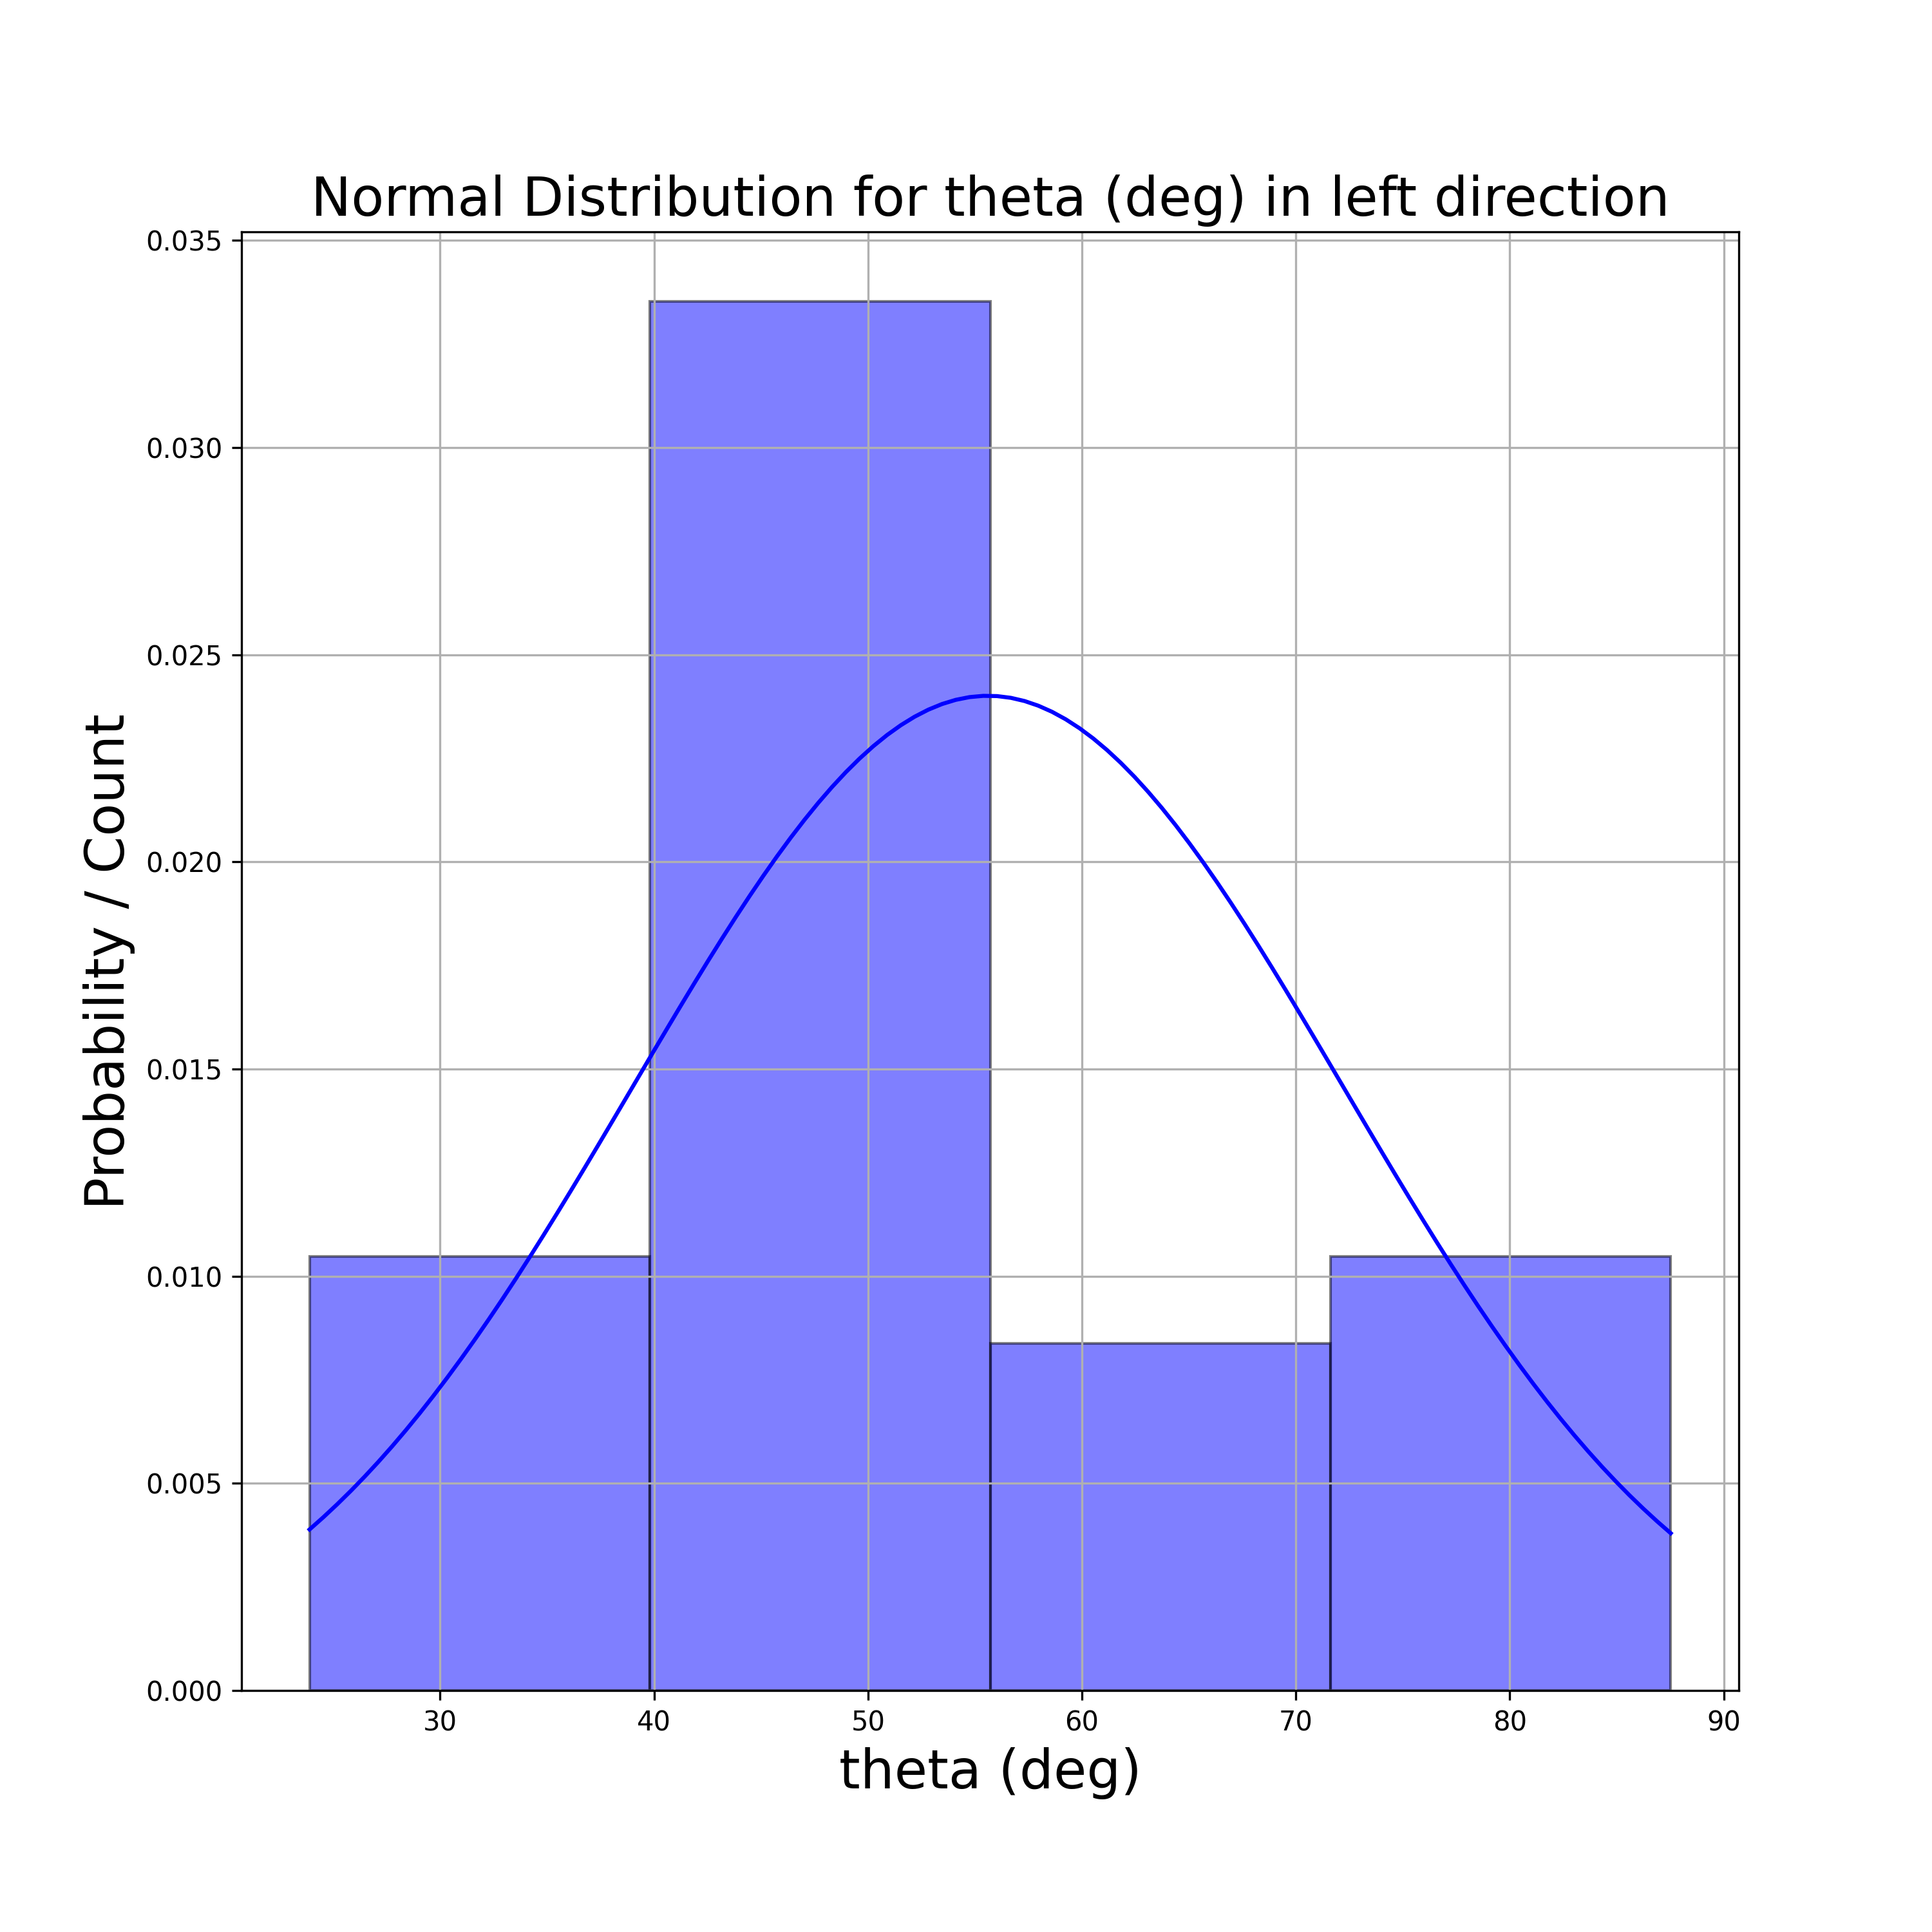
\includegraphics[ width=0.45\textwidth]{"images/experiment_3/normal_distribution_left_theta (deg).png"}}\\
    \caption{\textcolor{red}{Manually measured x, y and orientation in the left direction}}
        \label{guassianleft}
    \end{figure*}
    %000000000000000000000000000000000000000000000000000000000000000000000000000000000000%
    
    %000000000000000000000000000000000000000000000000000000000000000000000000000000000000%
    \begin{figure*}[ht!]
        \centering
       \subfloat[X-axis coordinates  \label{fig:guassianrightx}]{%
          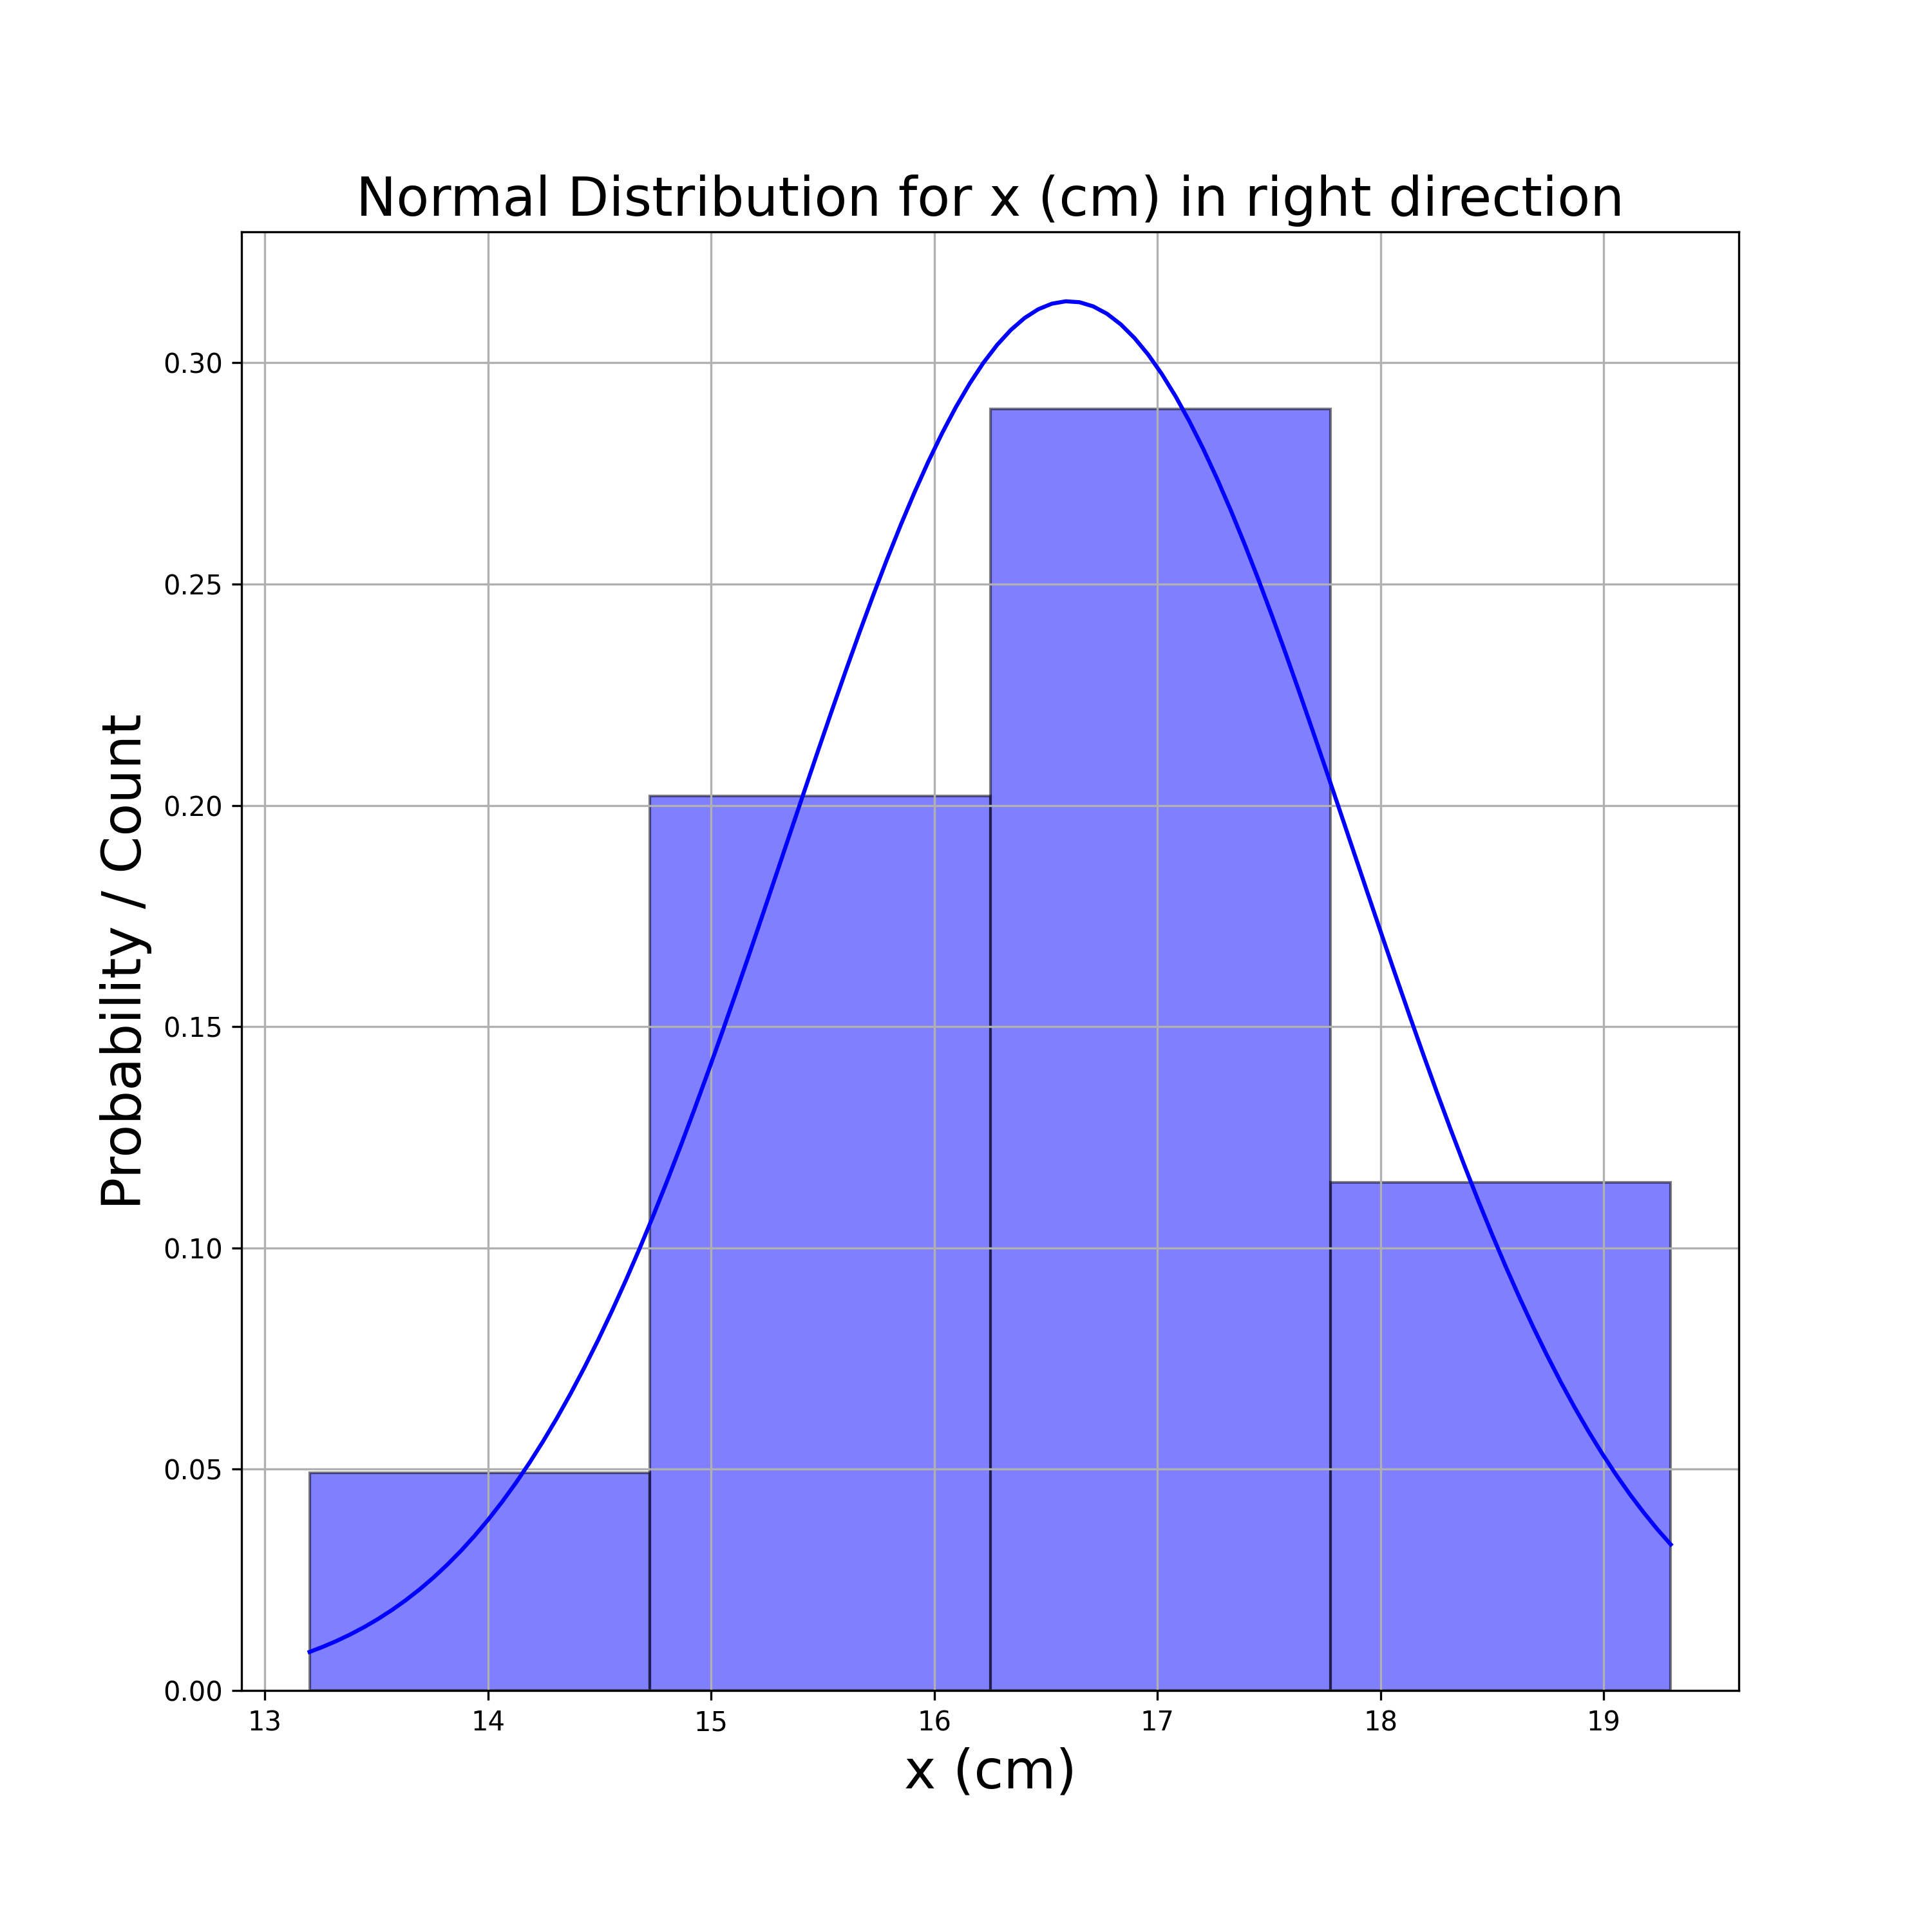
\includegraphics[ width=0.45\textwidth]{"images/experiment_3/normal_distribution_right_x (cm).png"}}
    \hspace{\fill}
       \subfloat[Y-axis coordinates  \label{fig:guassianrighty} ]{%
          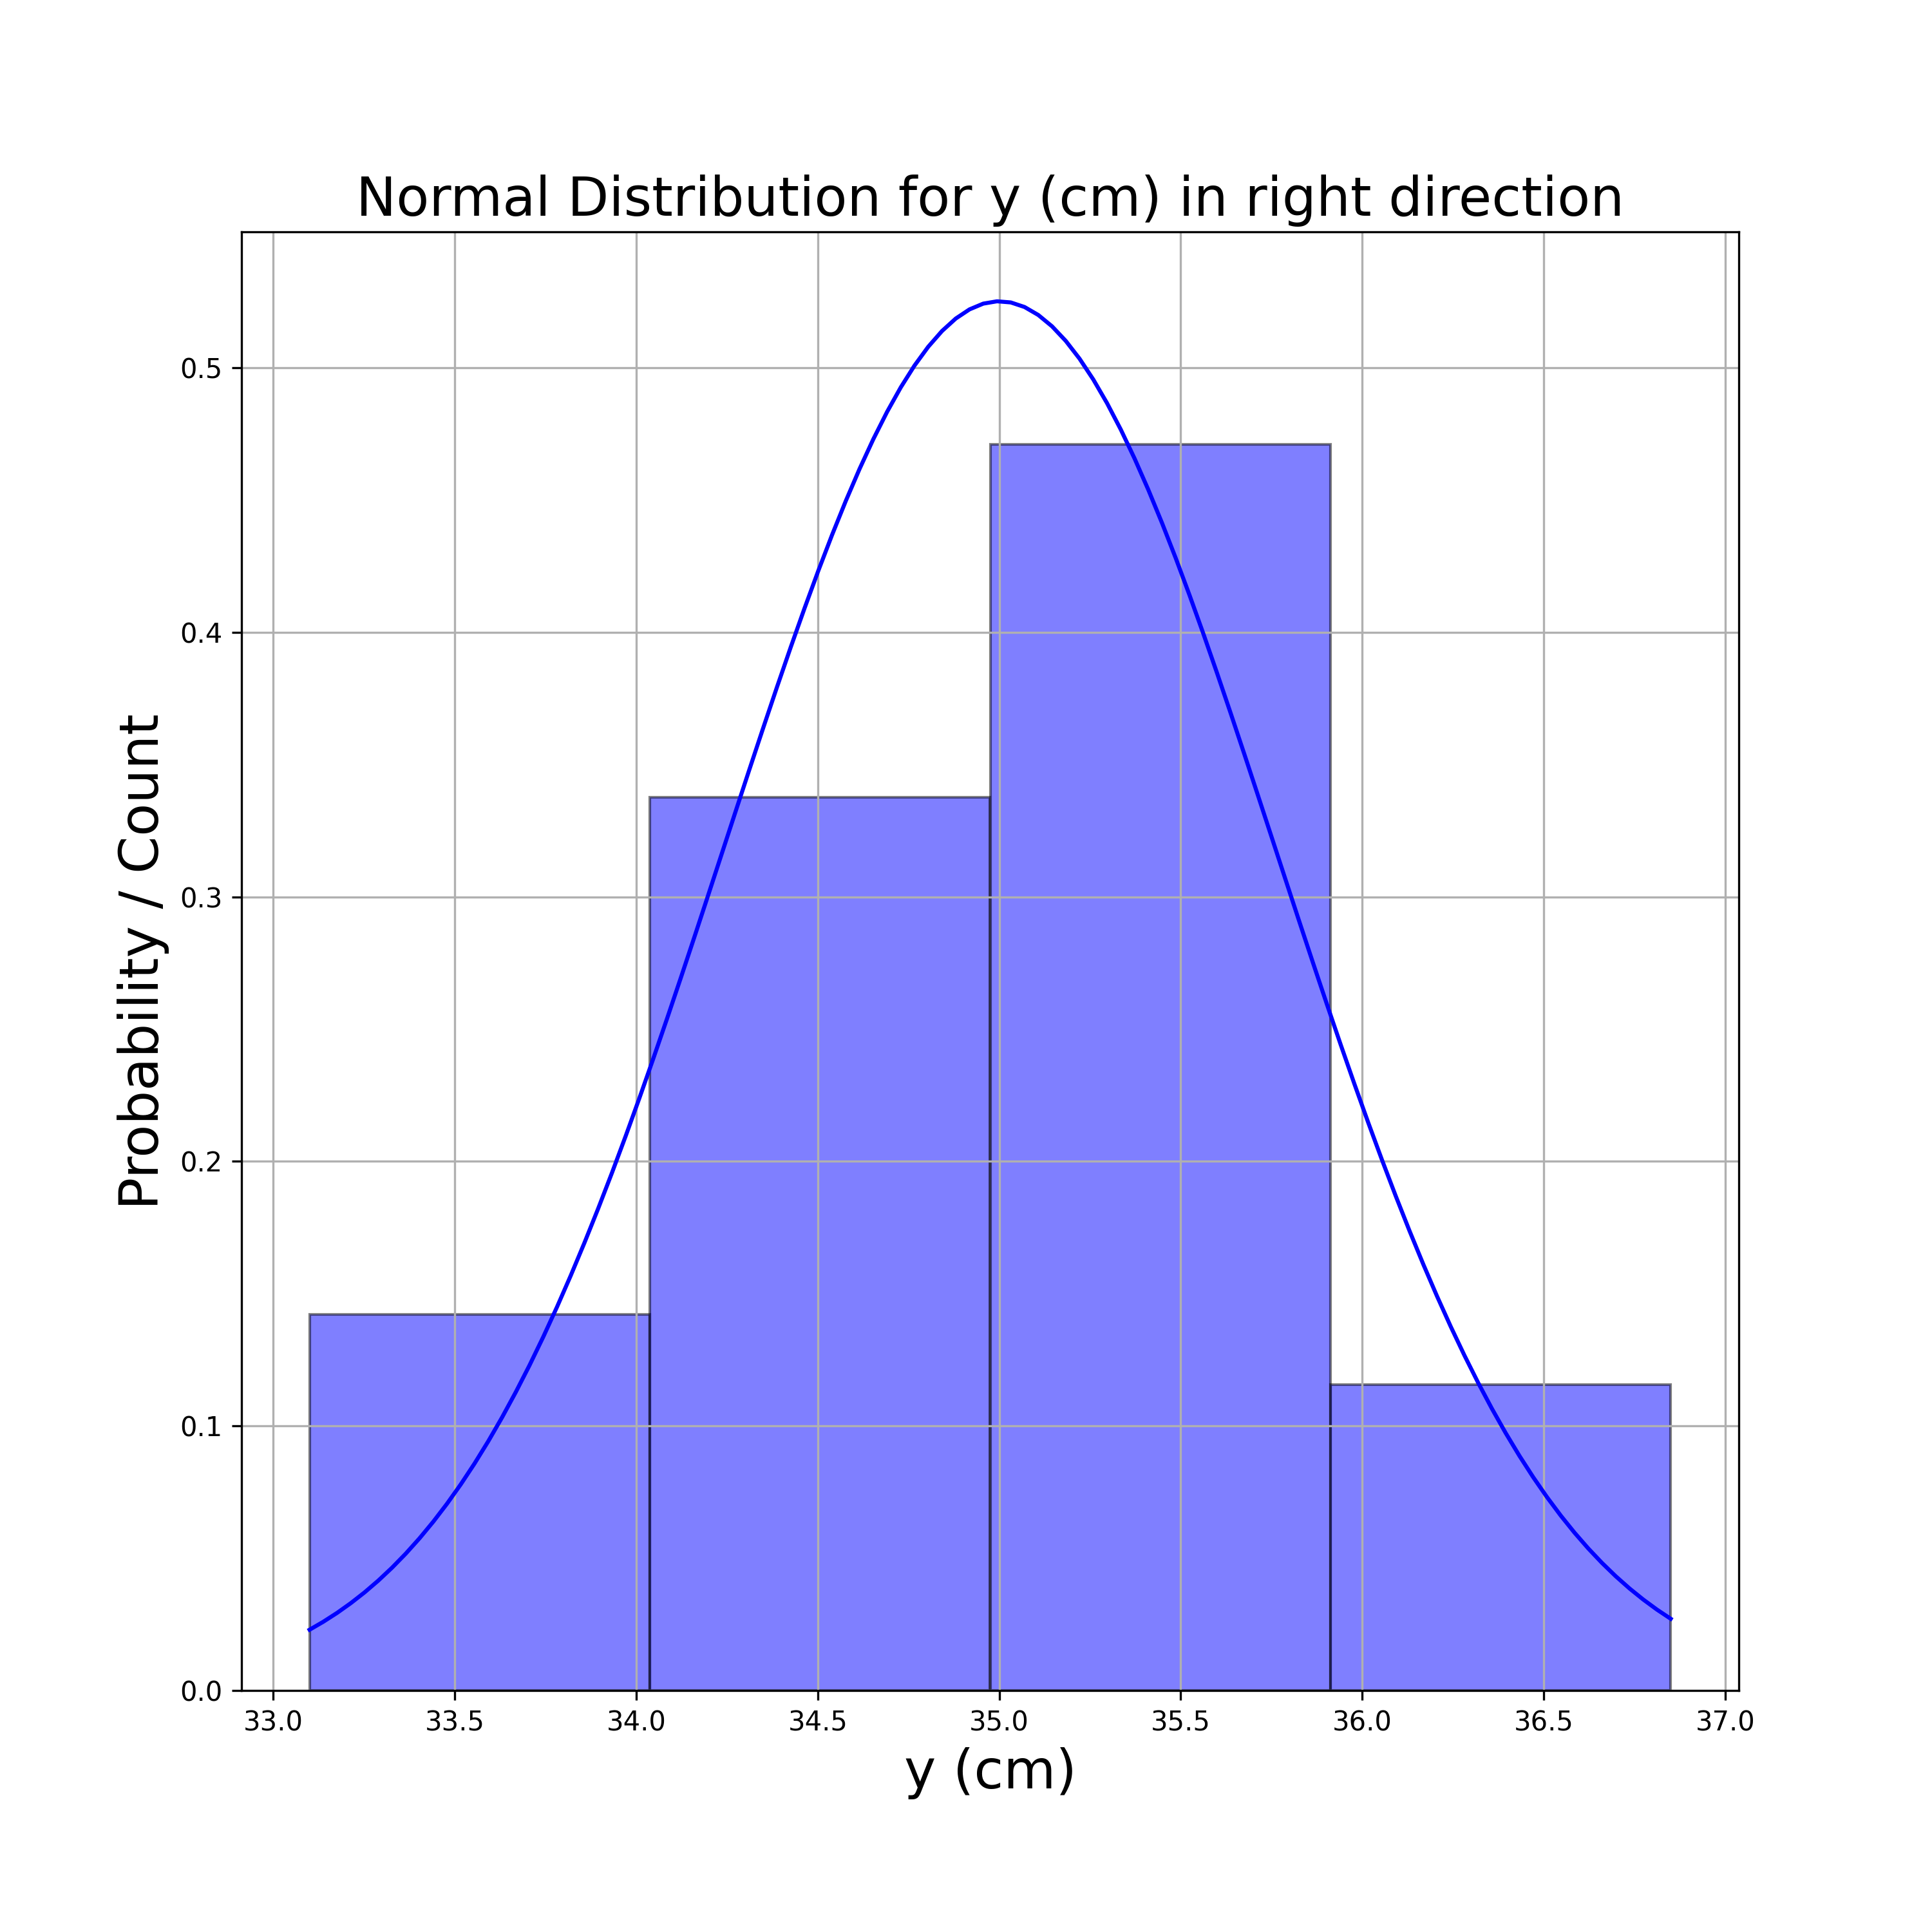
\includegraphics[ width=0.45\textwidth]{"images/experiment_3/normal_distribution_right_y (cm).png"}}
    \hspace{\fill}
       \subfloat[Orientation \label{fig:guassianrighttheta}]{%
          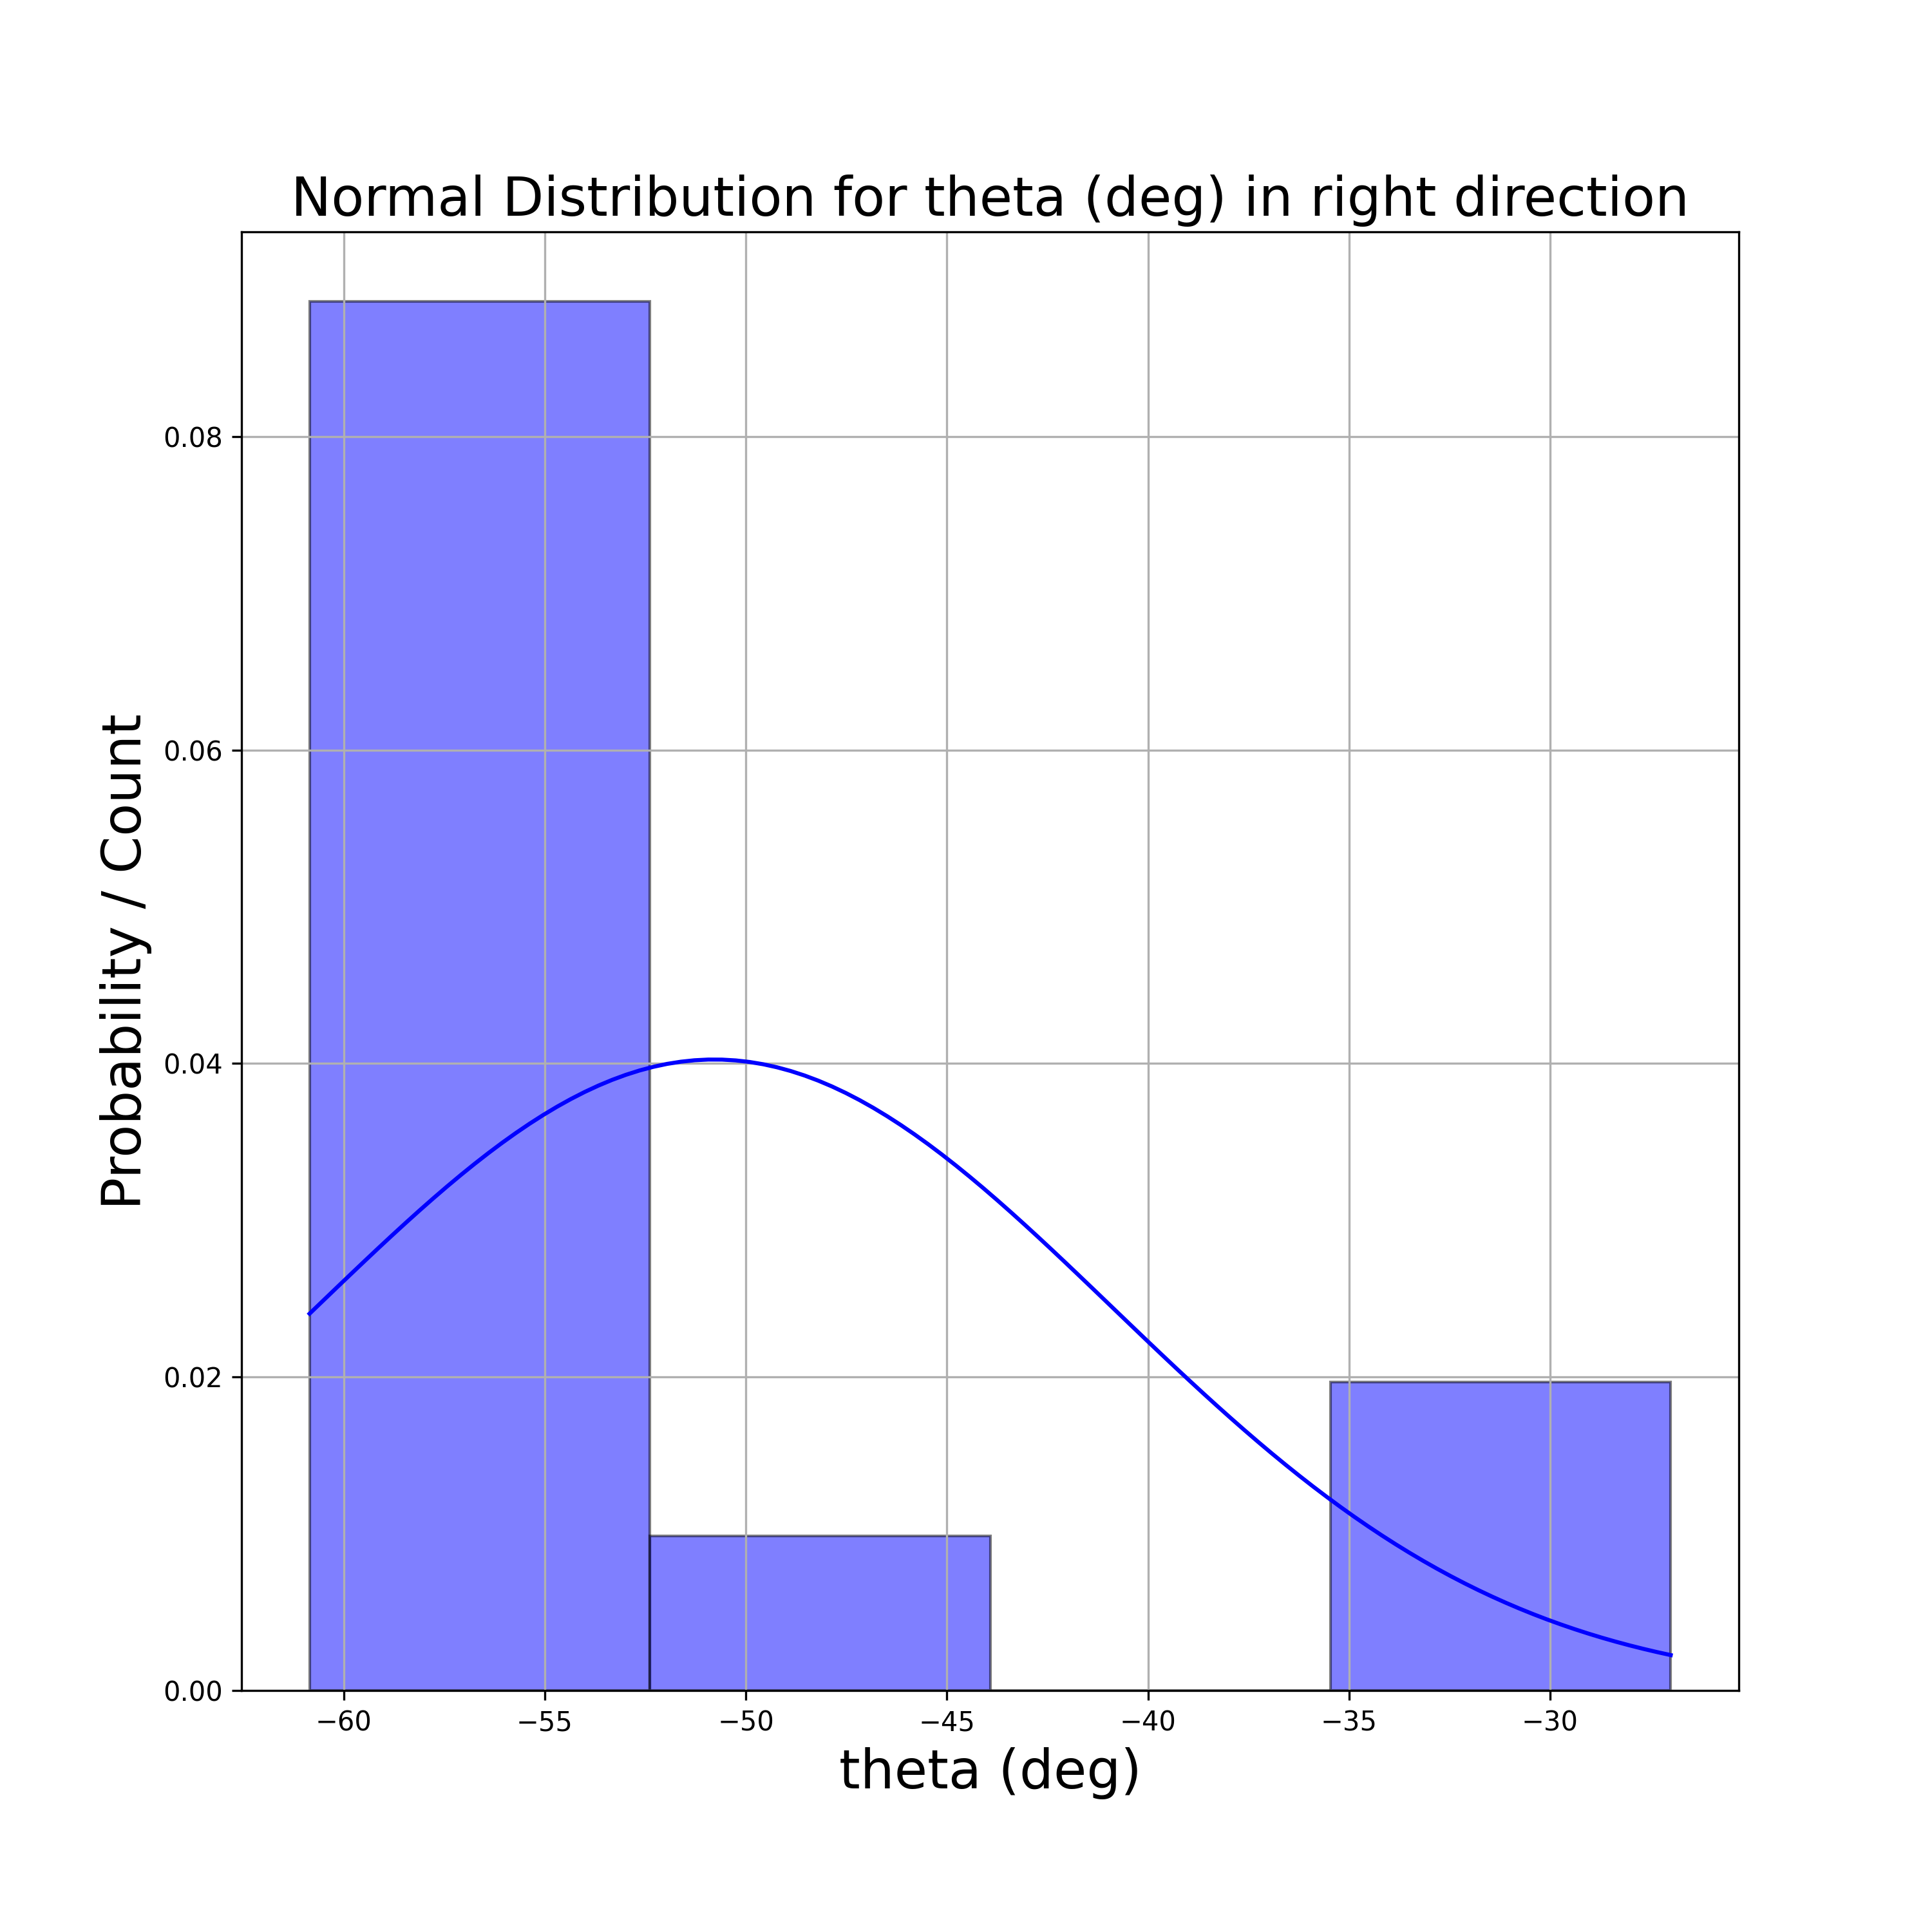
\includegraphics[ width=0.45\textwidth]{"images/experiment_3/normal_distribution_right_theta (deg).png"}}\\
    \caption{\textcolor{red}{Manually measured x, y and orientation in the right direction}}
        \label{guassianright}
    \end{figure*}
    %000000000000000000000000000000000000000000000000000000000000000000000000000000000000%
    
    
    %000000000000000000000000000000000000000000000000000000000000000000000000000000000000%
    \begin{figure}[!ht] 
            \centering 
            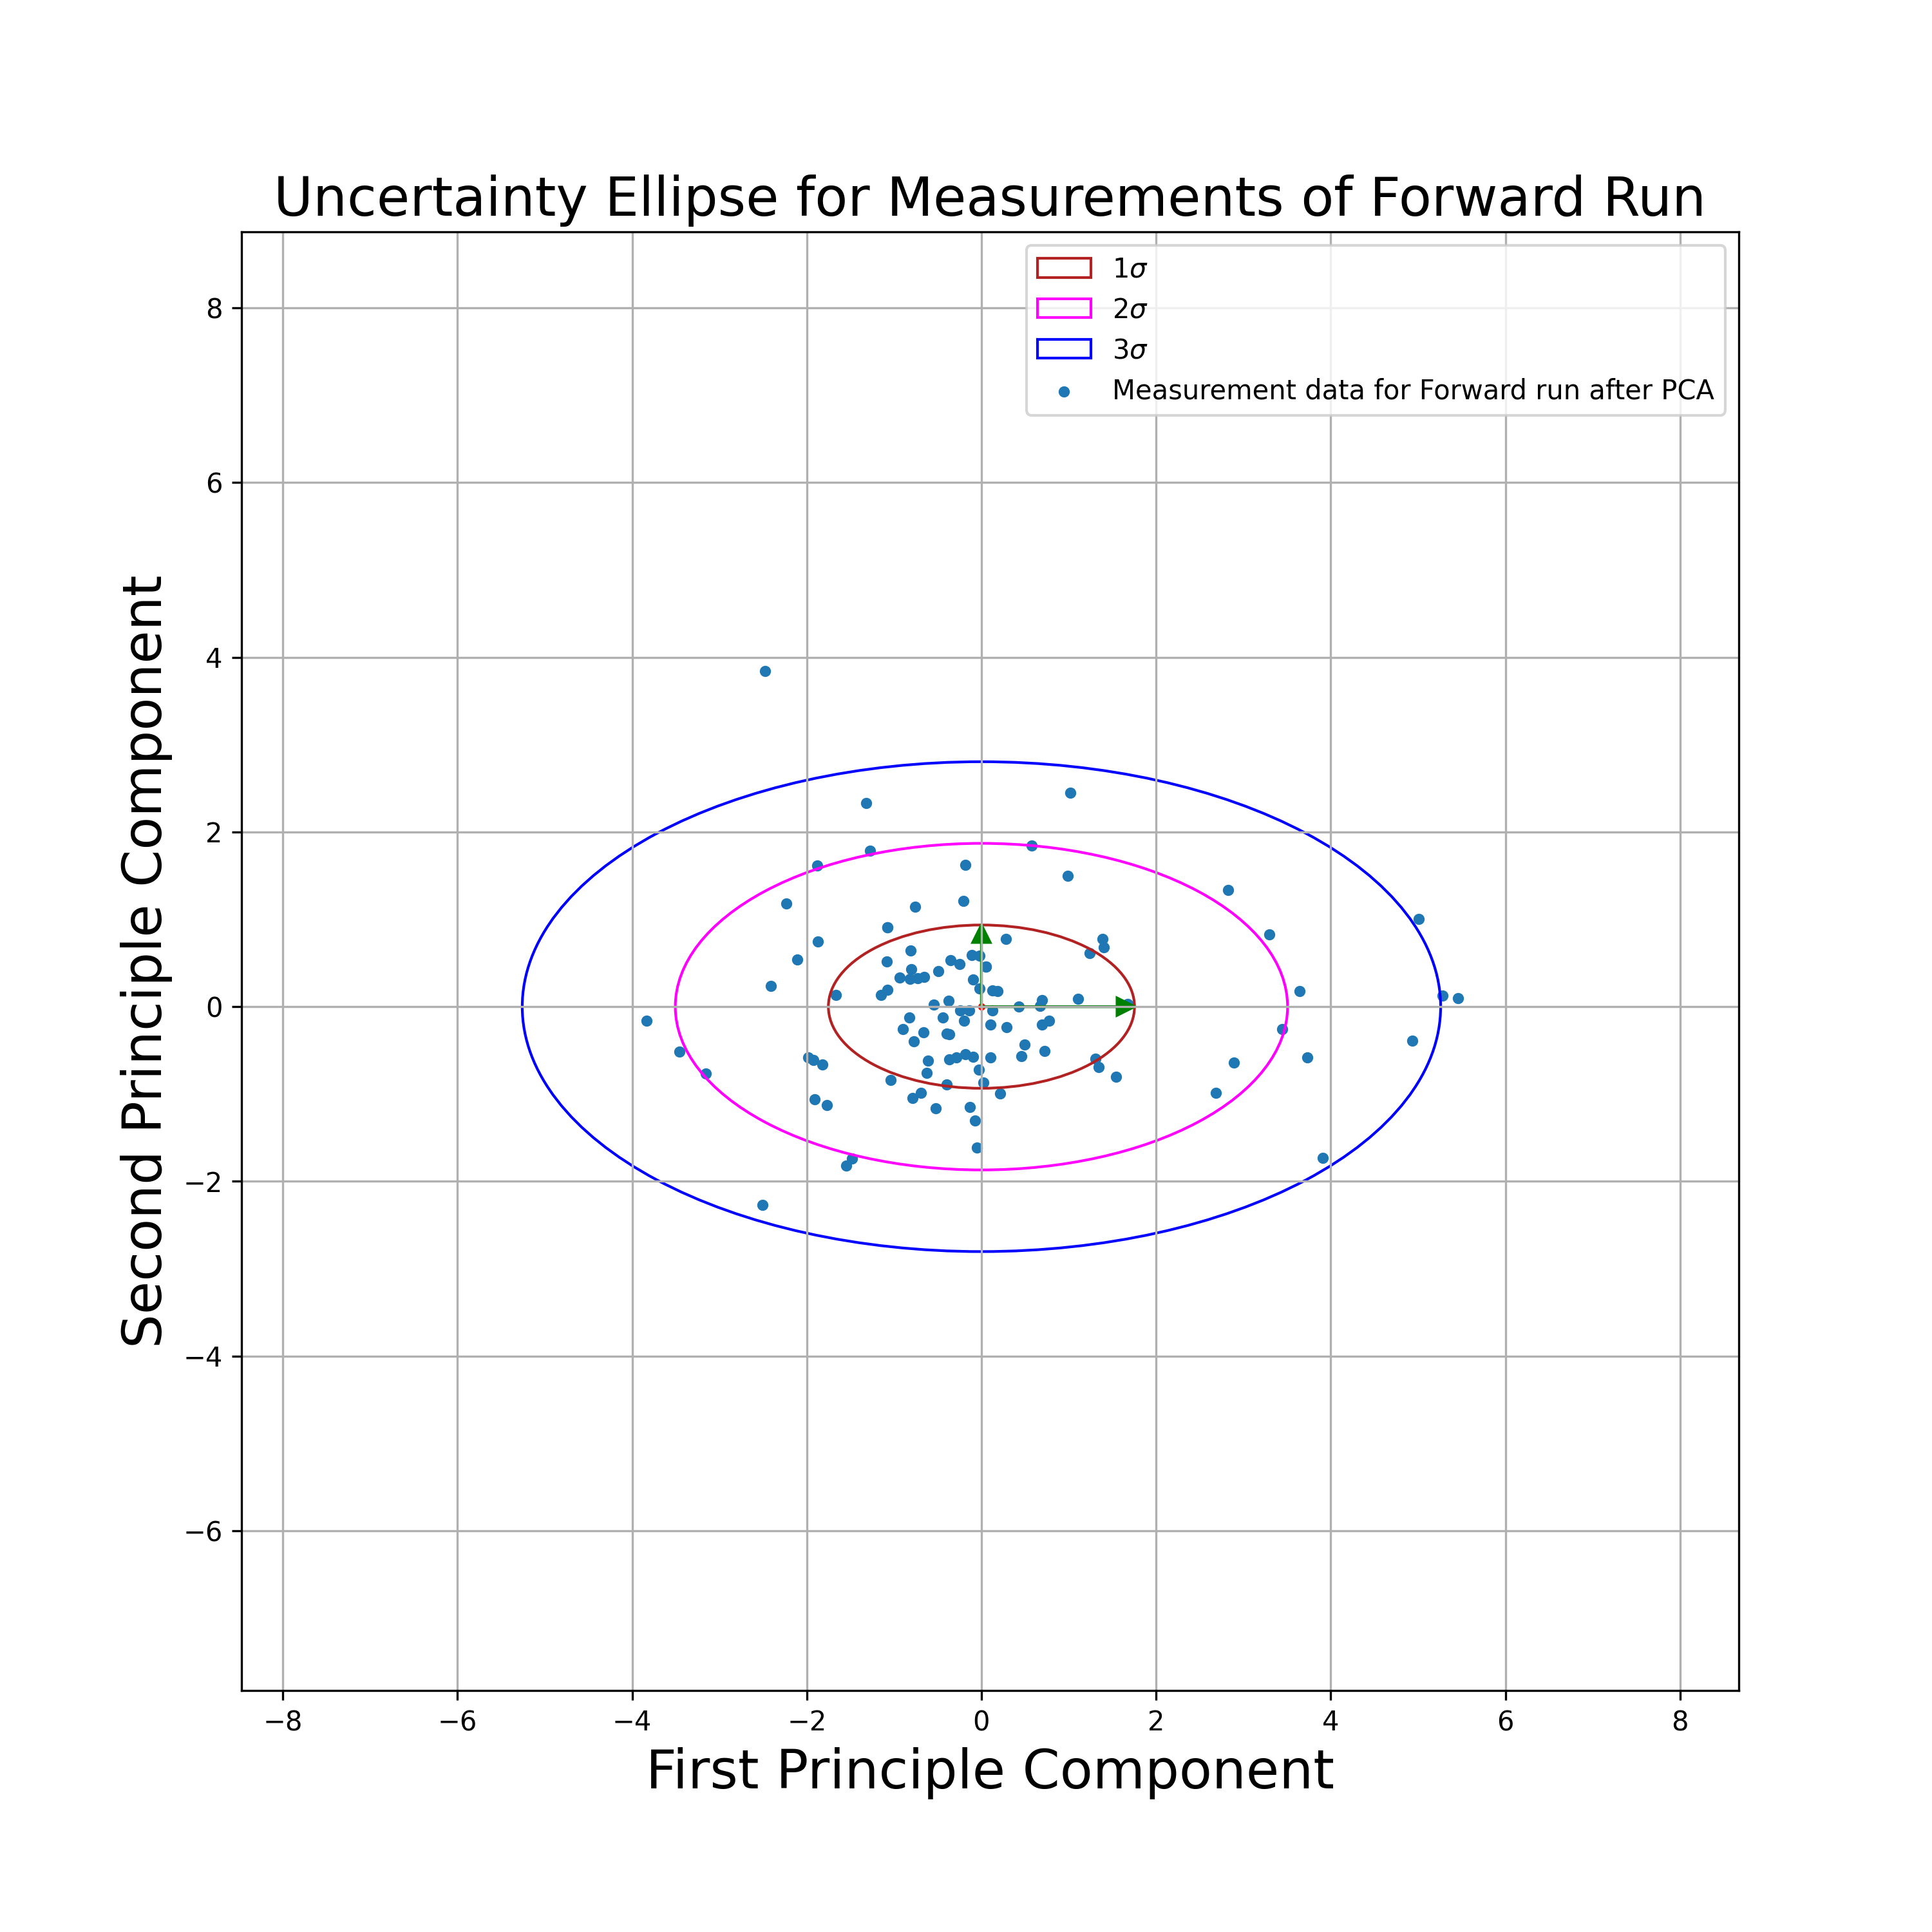
\includegraphics[width=0.8\textwidth]{"images/experiment_3/Uncertainty Ellipse for Measurements of Forward Run.png"}
            \caption{Forward Direction Measurements}
            \label{fig:ellipseforwardafter}
    \end{figure}
    \begin{figure}[!ht] 
            \centering 
            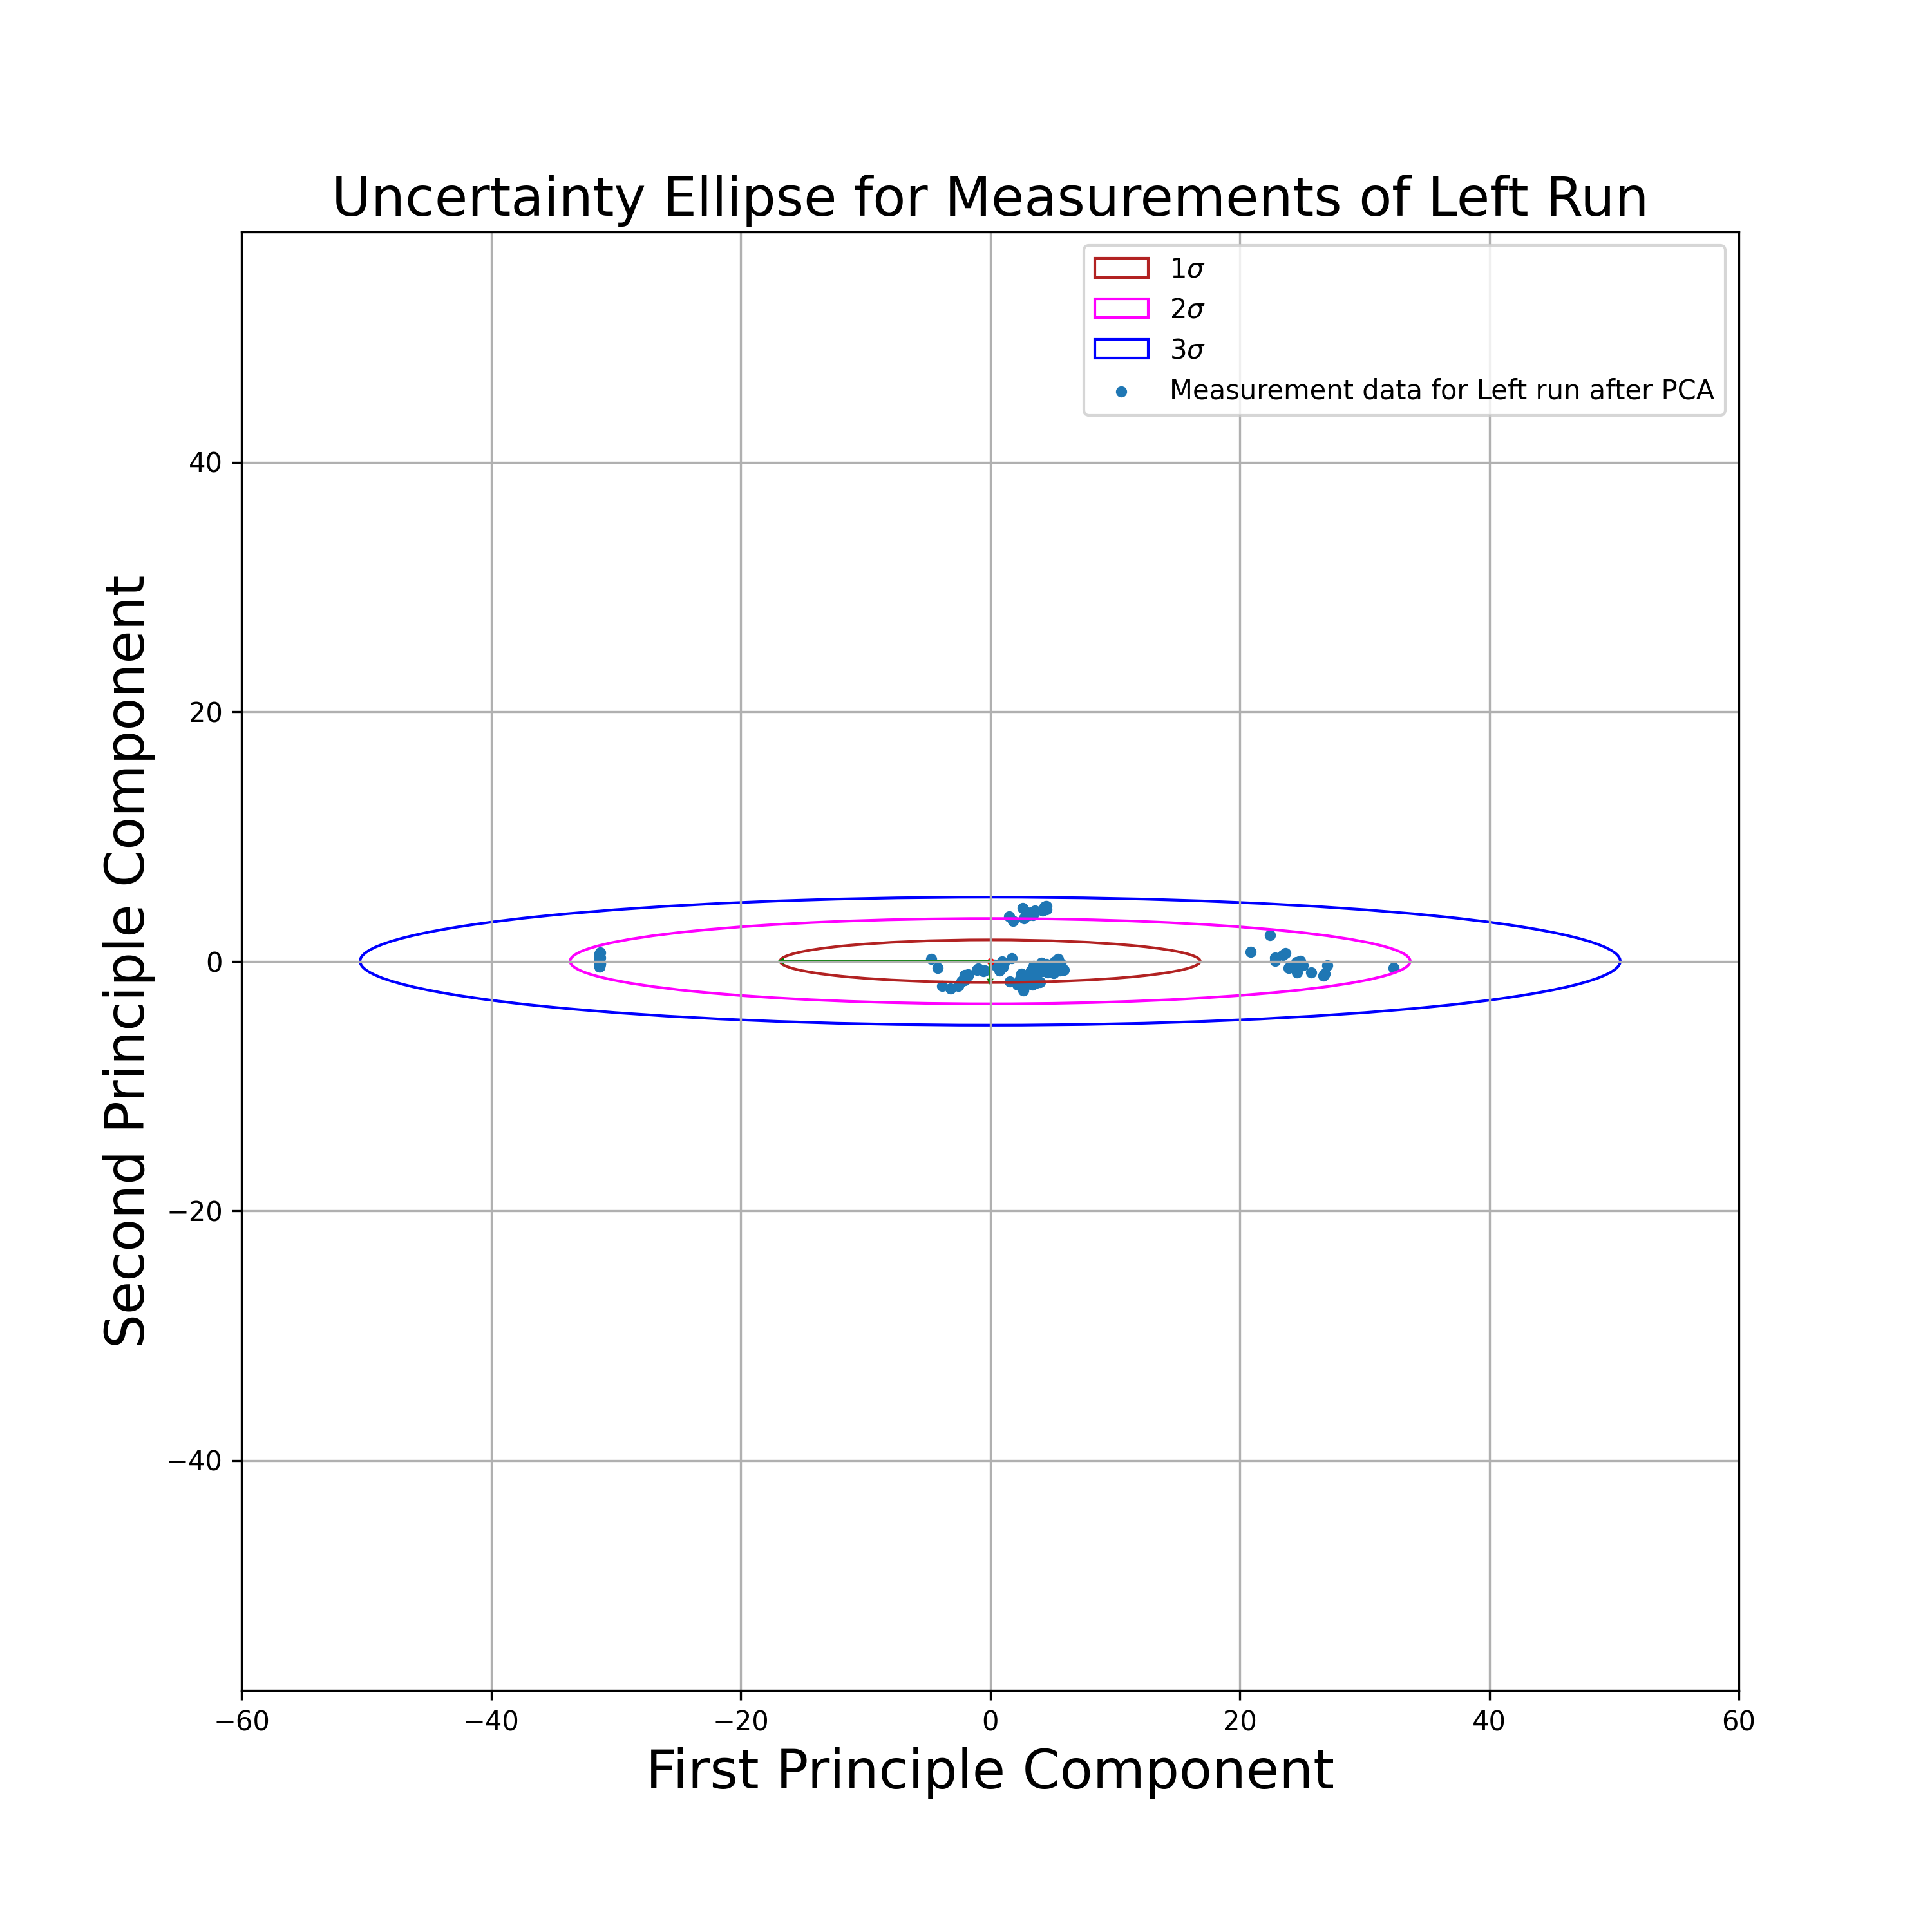
\includegraphics[width=0.8\textwidth]{"images/experiment_3/Uncertainty Ellipse for Measurements of Left Run.png"}
            \caption{Left Direction Measurements}
            \label{fig:ellipseleftafter}
    \end{figure}
    \begin{figure}[!ht] 
            \centering 
            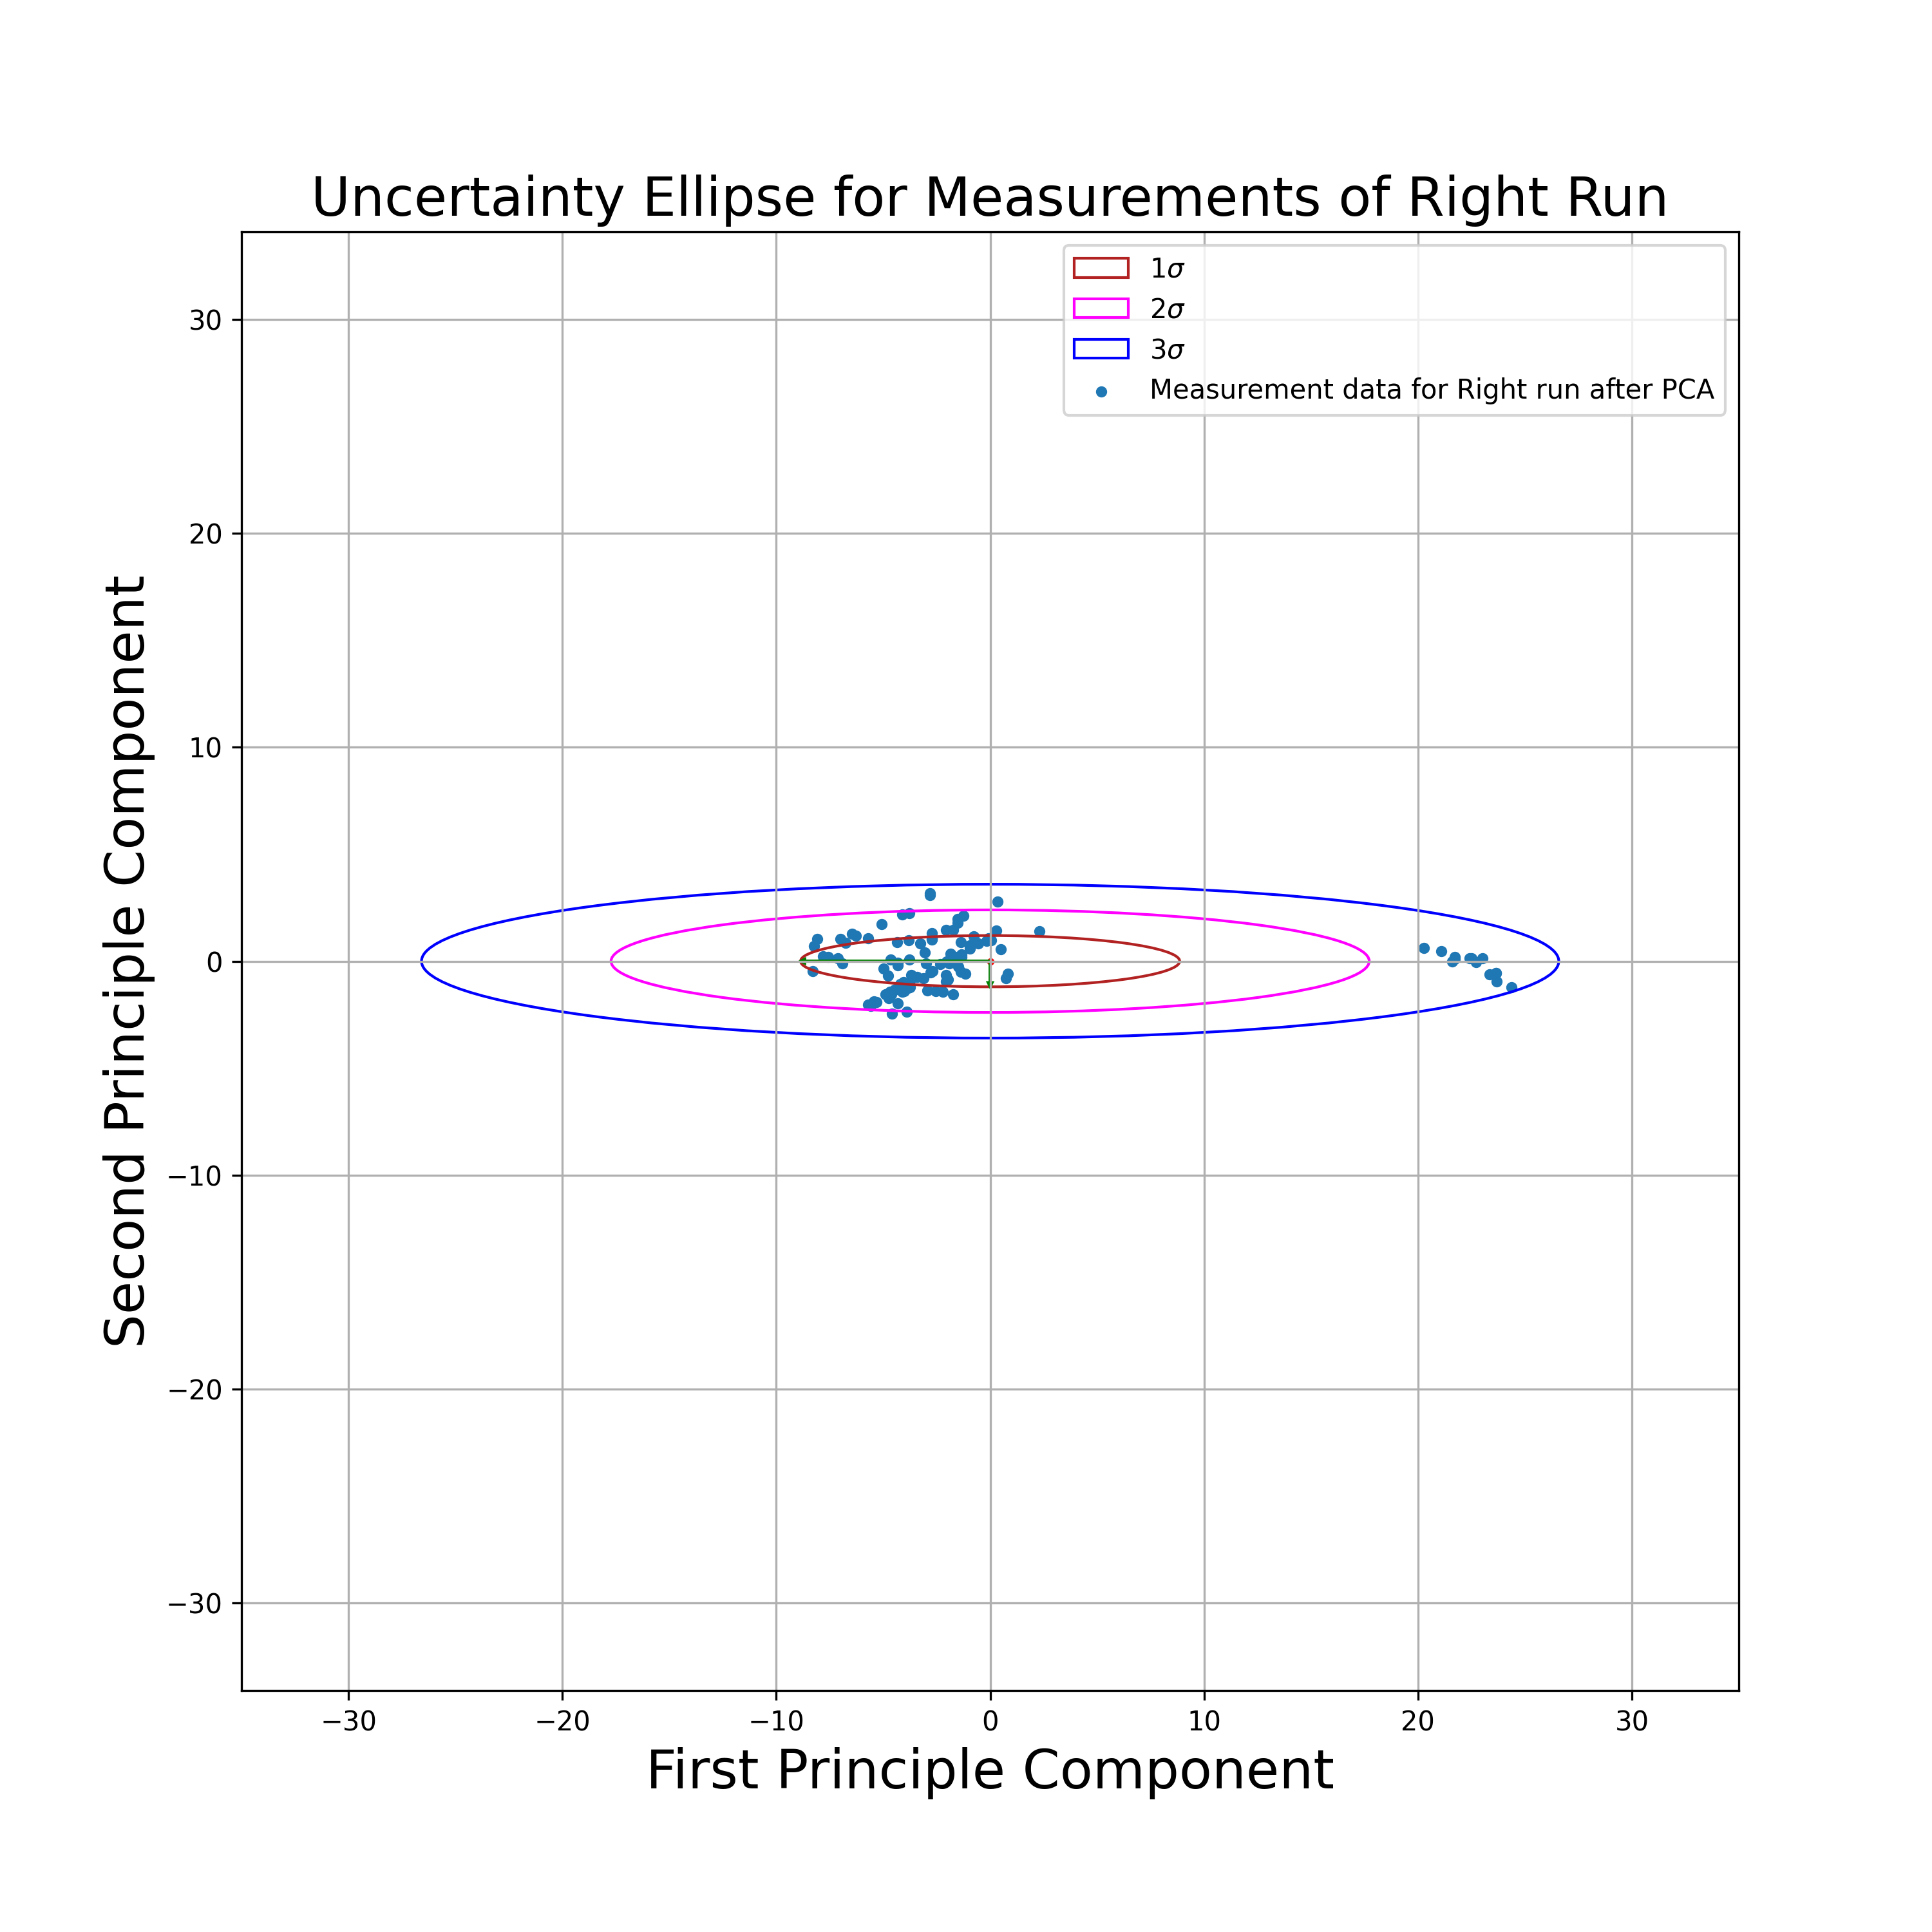
\includegraphics[width=0.8\textwidth]{"images/experiment_3/Uncertainty Ellipse for Measurements of Right Run.png"}
            \caption{Right Direction Measurements}
            \label{fig:ellipserightafter}
    \end{figure}
    % \begin{figure*}[ht!]
    % \centering
    %   \subfloat[Forward Direction Measurements\label{fig:ellipseforwardafter}]{%
    %       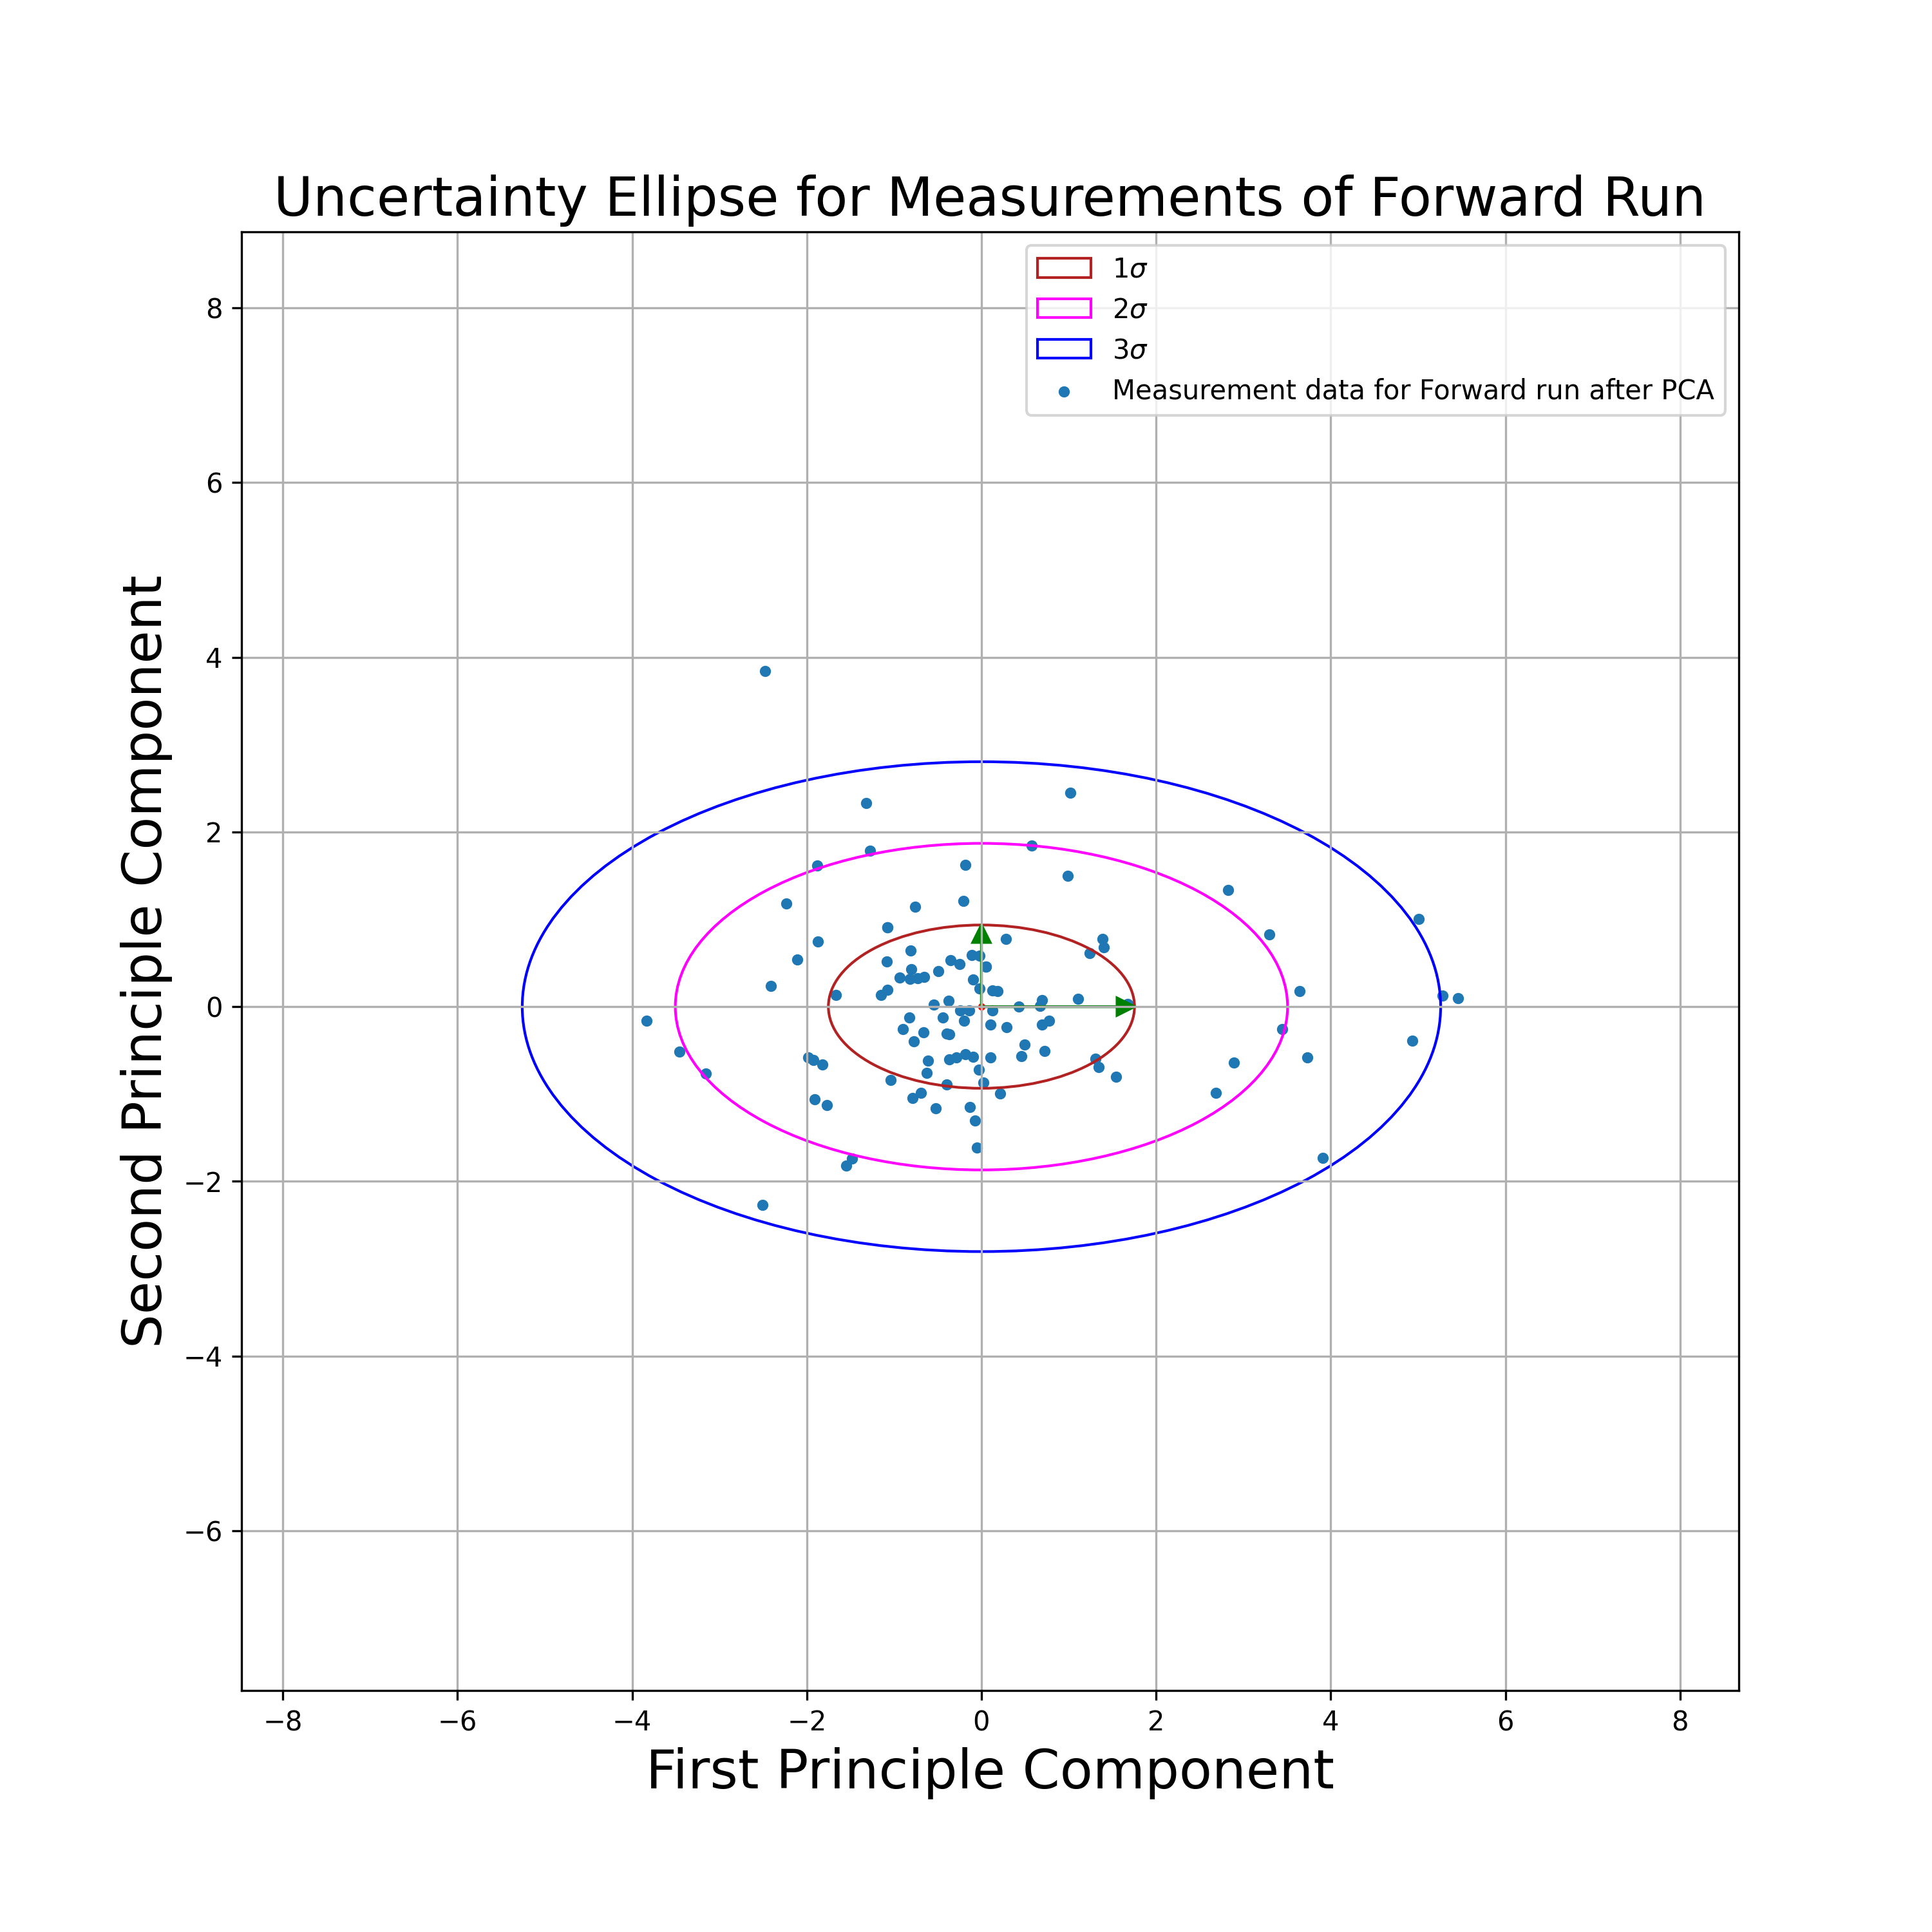
\includegraphics[ width=0.45\textwidth]{"images/experiment_3/Uncertainty Ellipse for Measurements of Forward Run.png"}}
    % \hspace{\fill}
    %   \subfloat[Left Direction Measurements \label{fig:ellipseleftafter} ]{%
    %       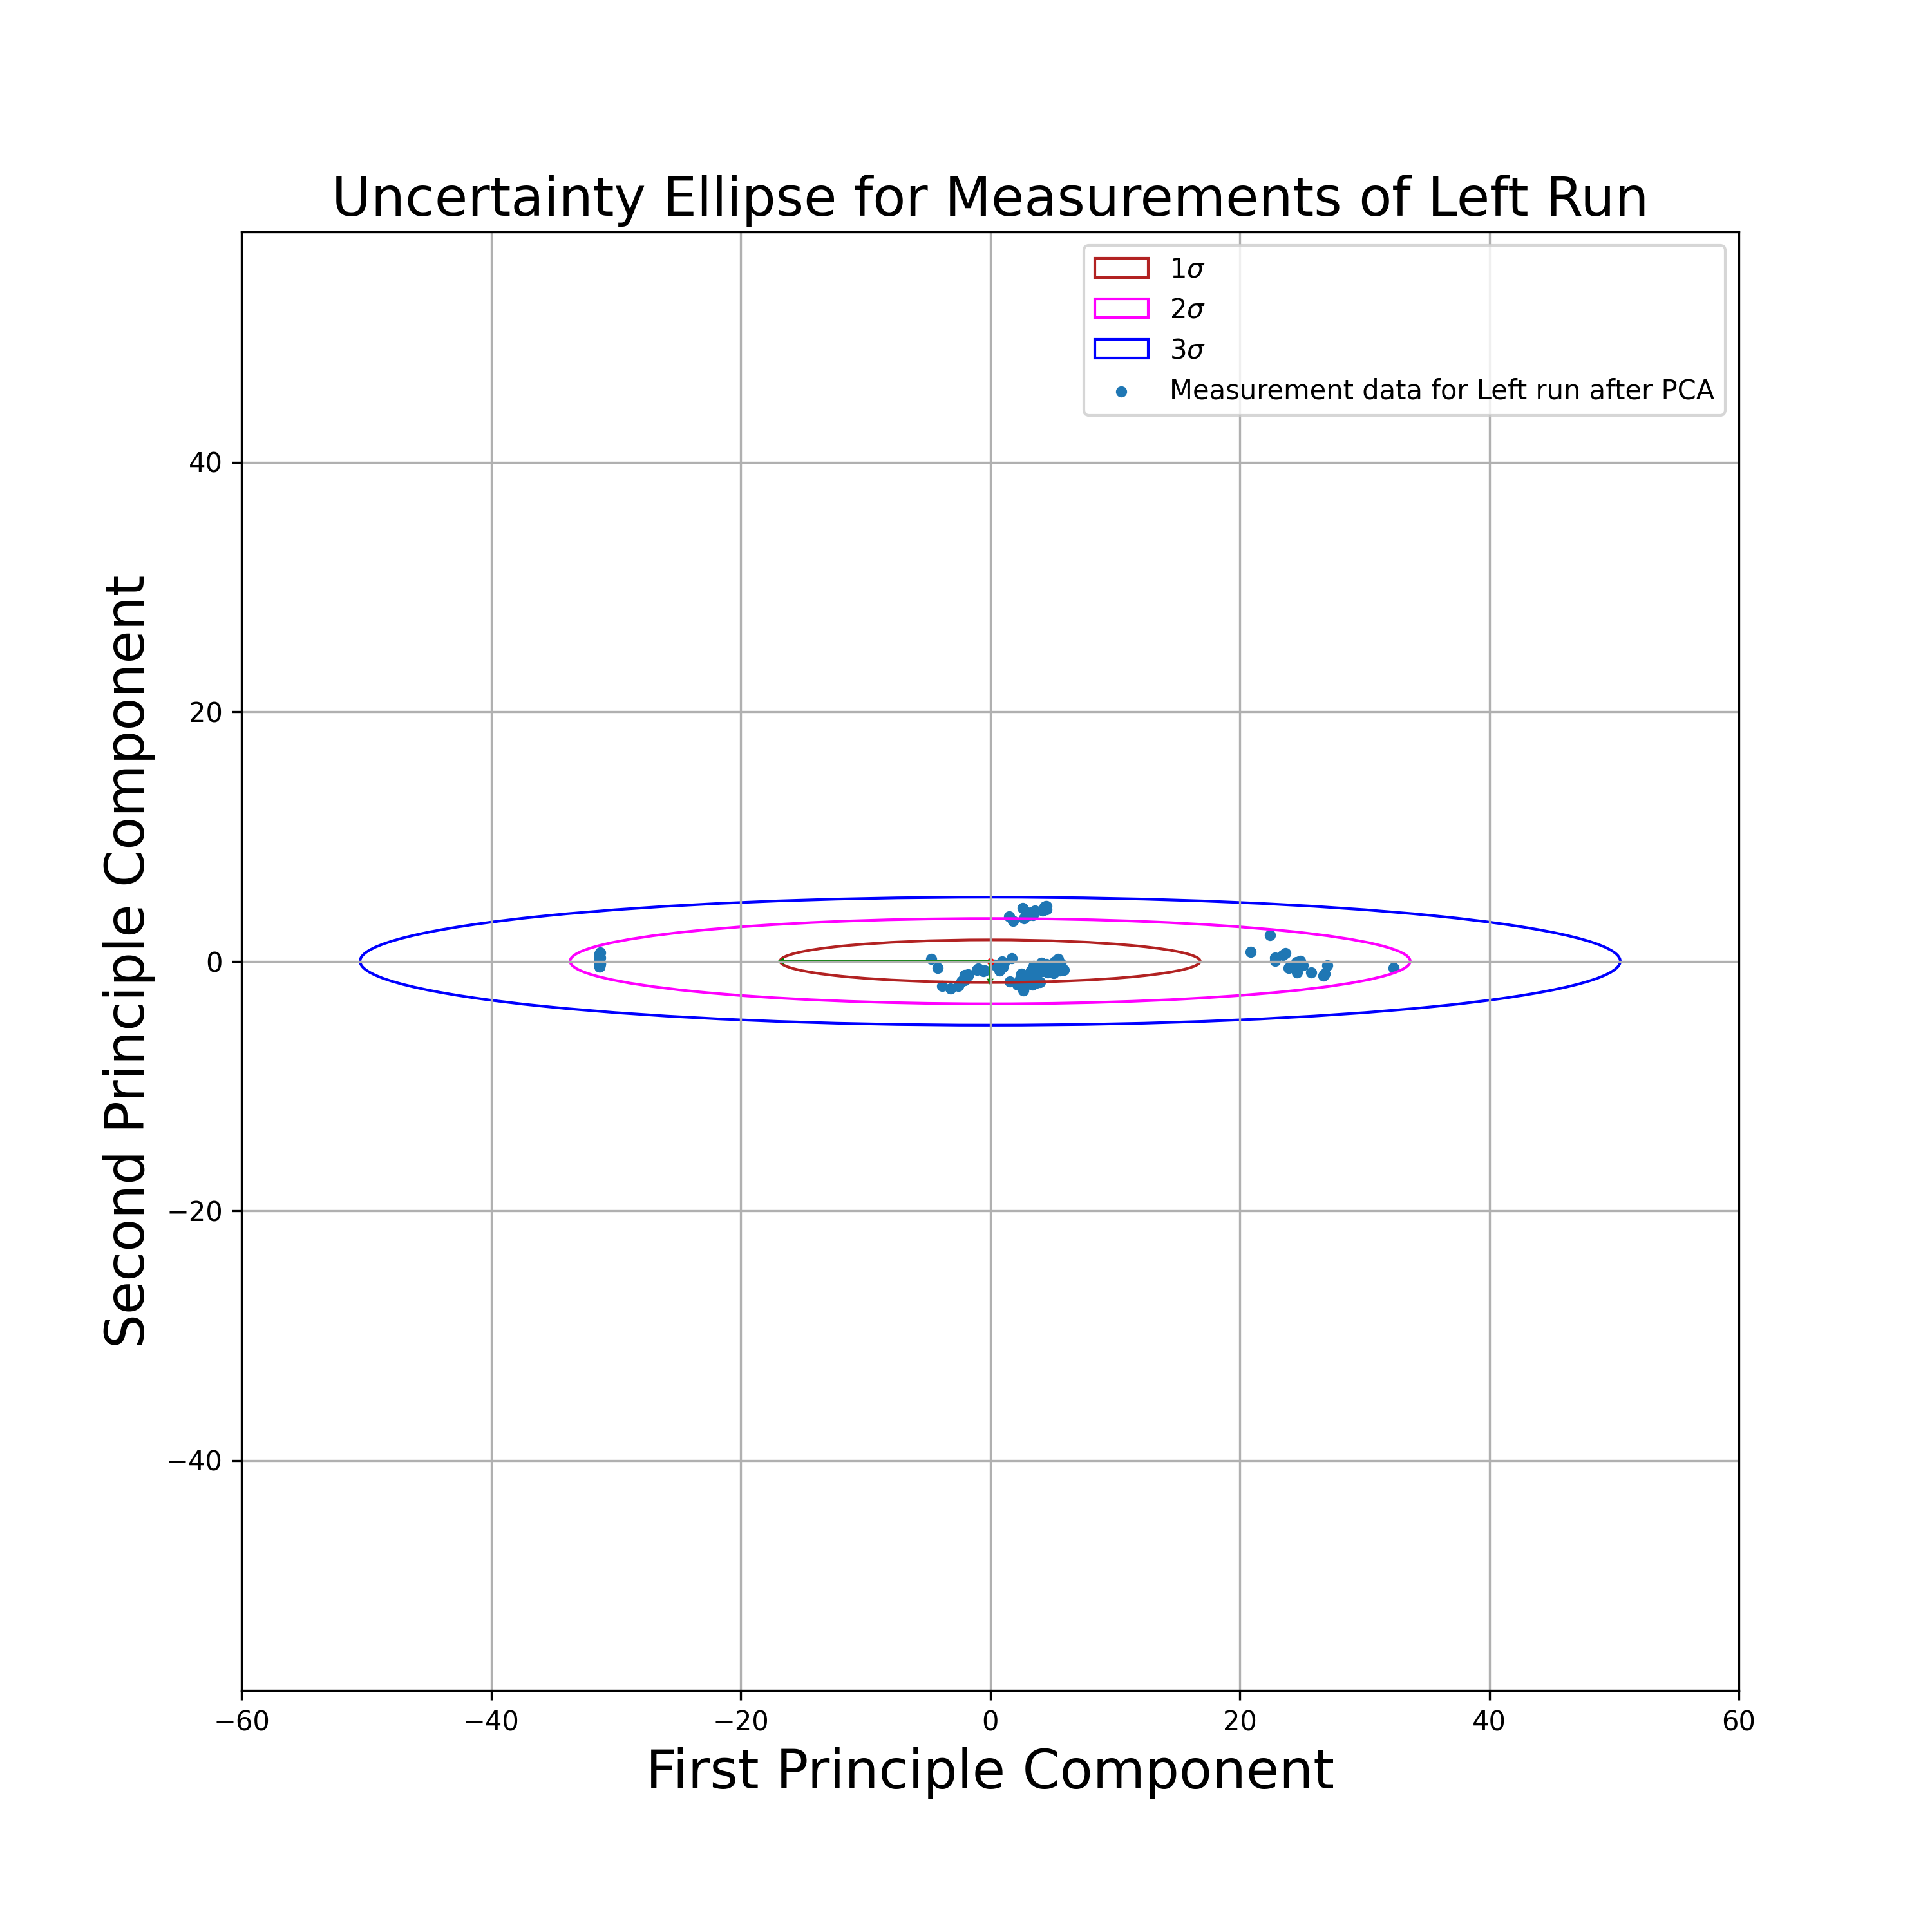
\includegraphics[ width=0.45\textwidth]{"images/experiment_3/Uncertainty Ellipse for Measurements of Left Run.png"}}
    % \hspace{\fill}
    %   \subfloat[Right Direction Measurements \label{fig:ellipserightafter}]{%
    %       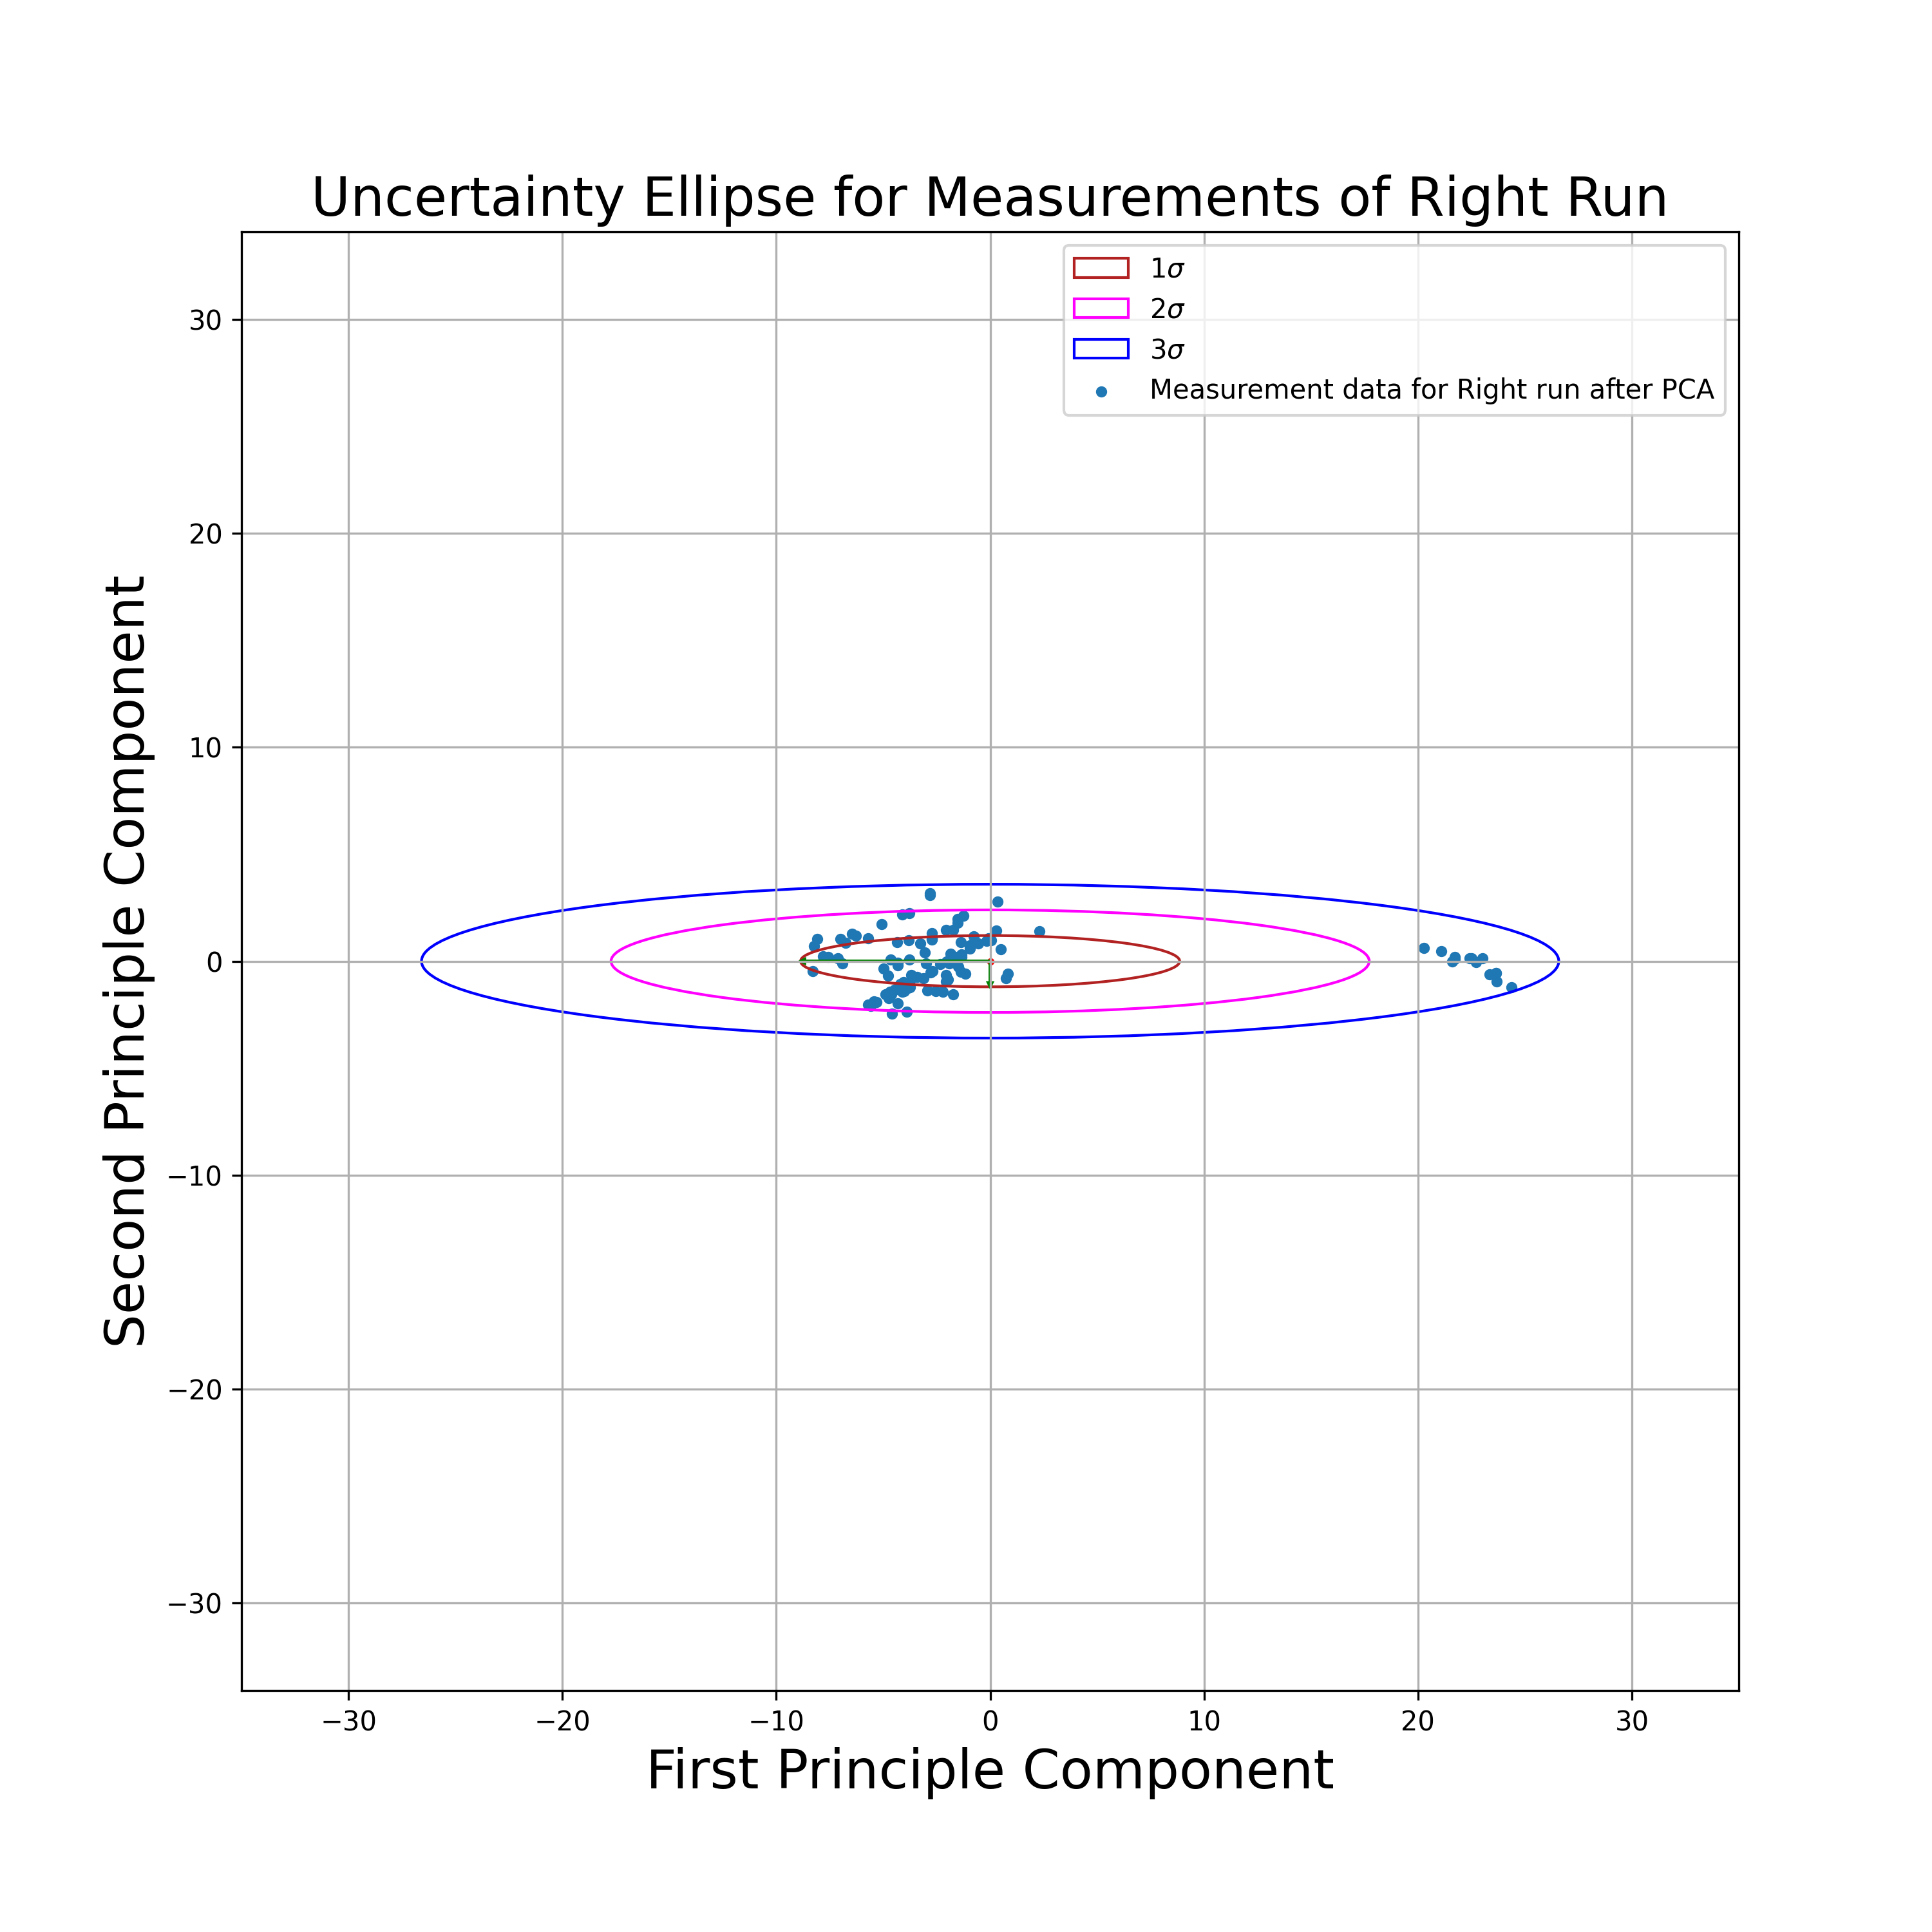
\includegraphics[ width=0.45\textwidth]{"images/experiment_3/Uncertainty Ellipse for Measurements of Right Run.png"}}\\
    % \caption{Uncertanity Ellipses for the measurements after PCA}
    %     \label{workflow}
    % \end{figure*}
    %000000000000000000000000000000000000000000000000000000000000000000000000000000000000%
    
    \begin{figure}[!ht] 
            \centering 
            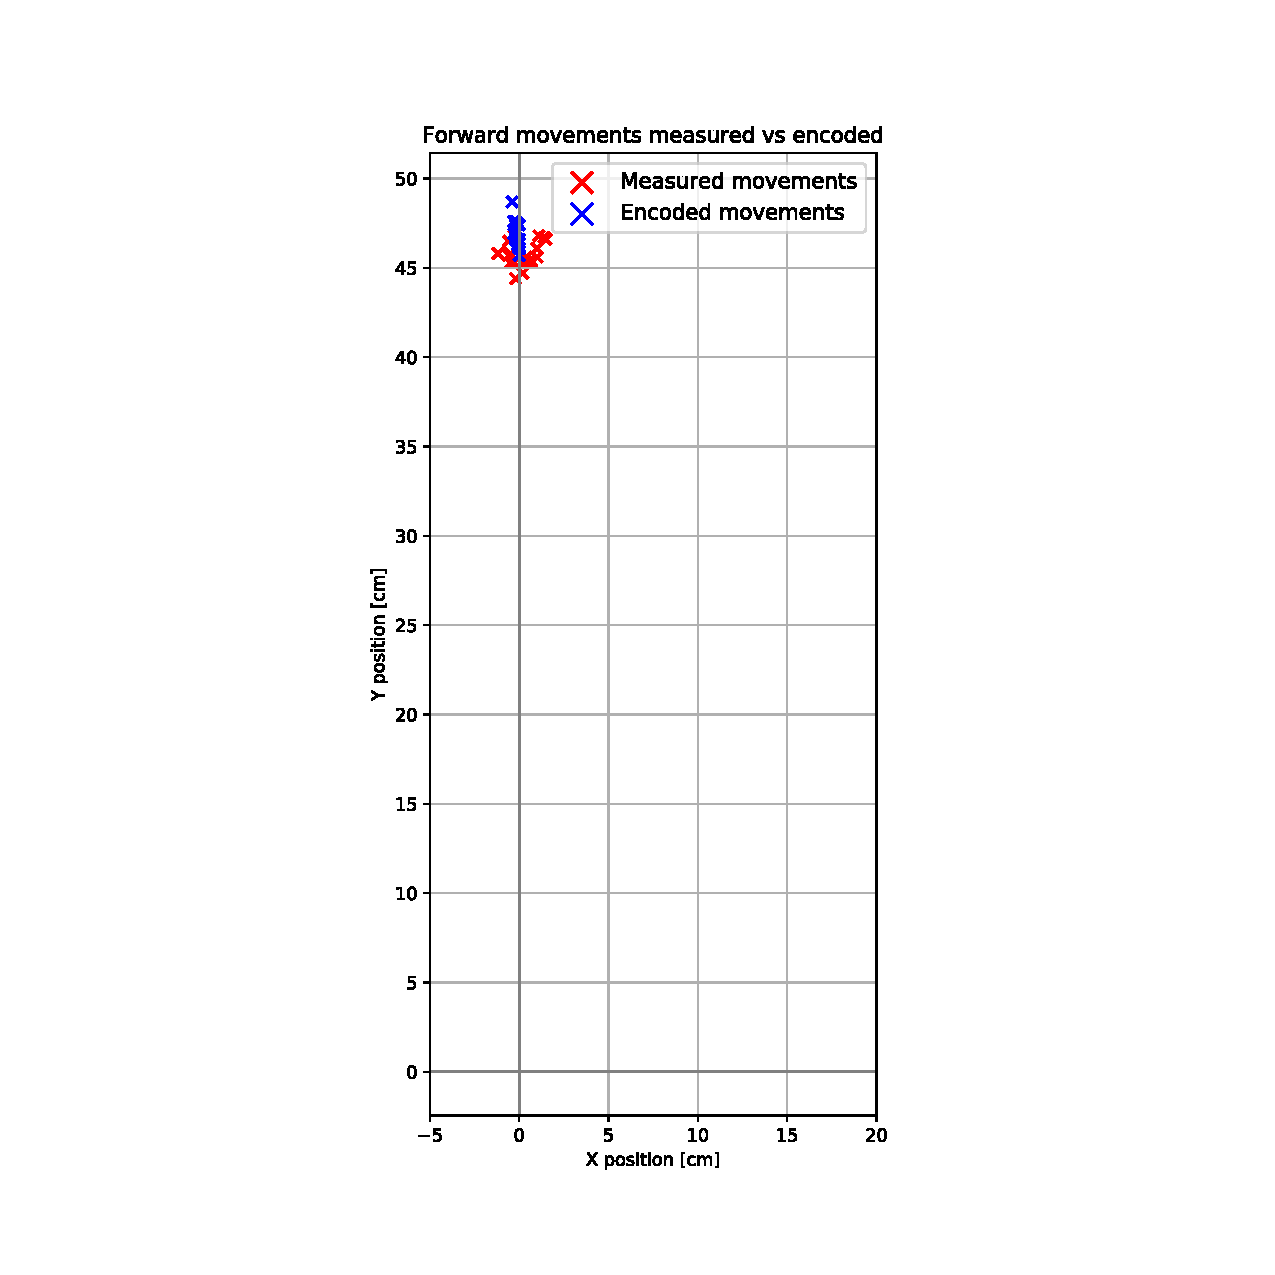
\includegraphics[page={1}, scale=.50]{images/pdf/forward_movements_measured_and_encoded.pdf}
            \caption{Visualising the manually measured forward poses and encoder logs}
            \label{fig:encoder-1}
    \end{figure}
    
      \begin{figure}[!ht] 
            \centering 
            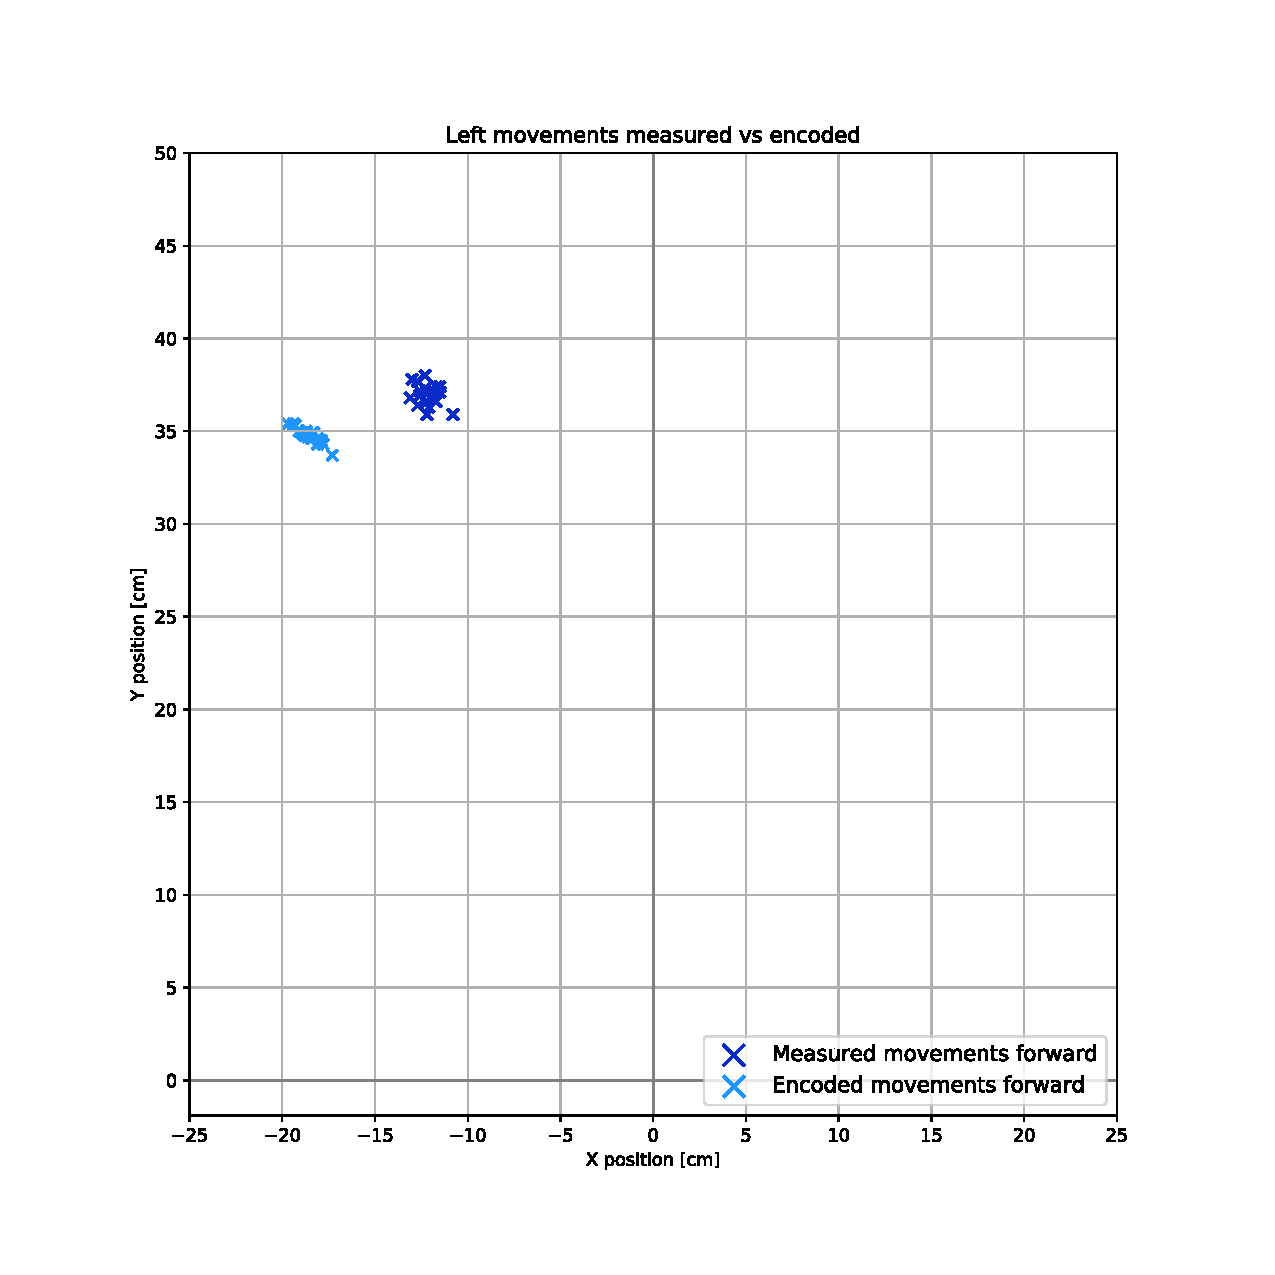
\includegraphics[page={1}, scale=.50]{images/pdf/left_movements_measured_and_encoded.pdf}
            \caption{Visualising the manually measured left poses and encoder logs}
            \label{fig:encoder-2}
    \end{figure}
    
        
      \begin{figure}[!ht] 
            \centering 
            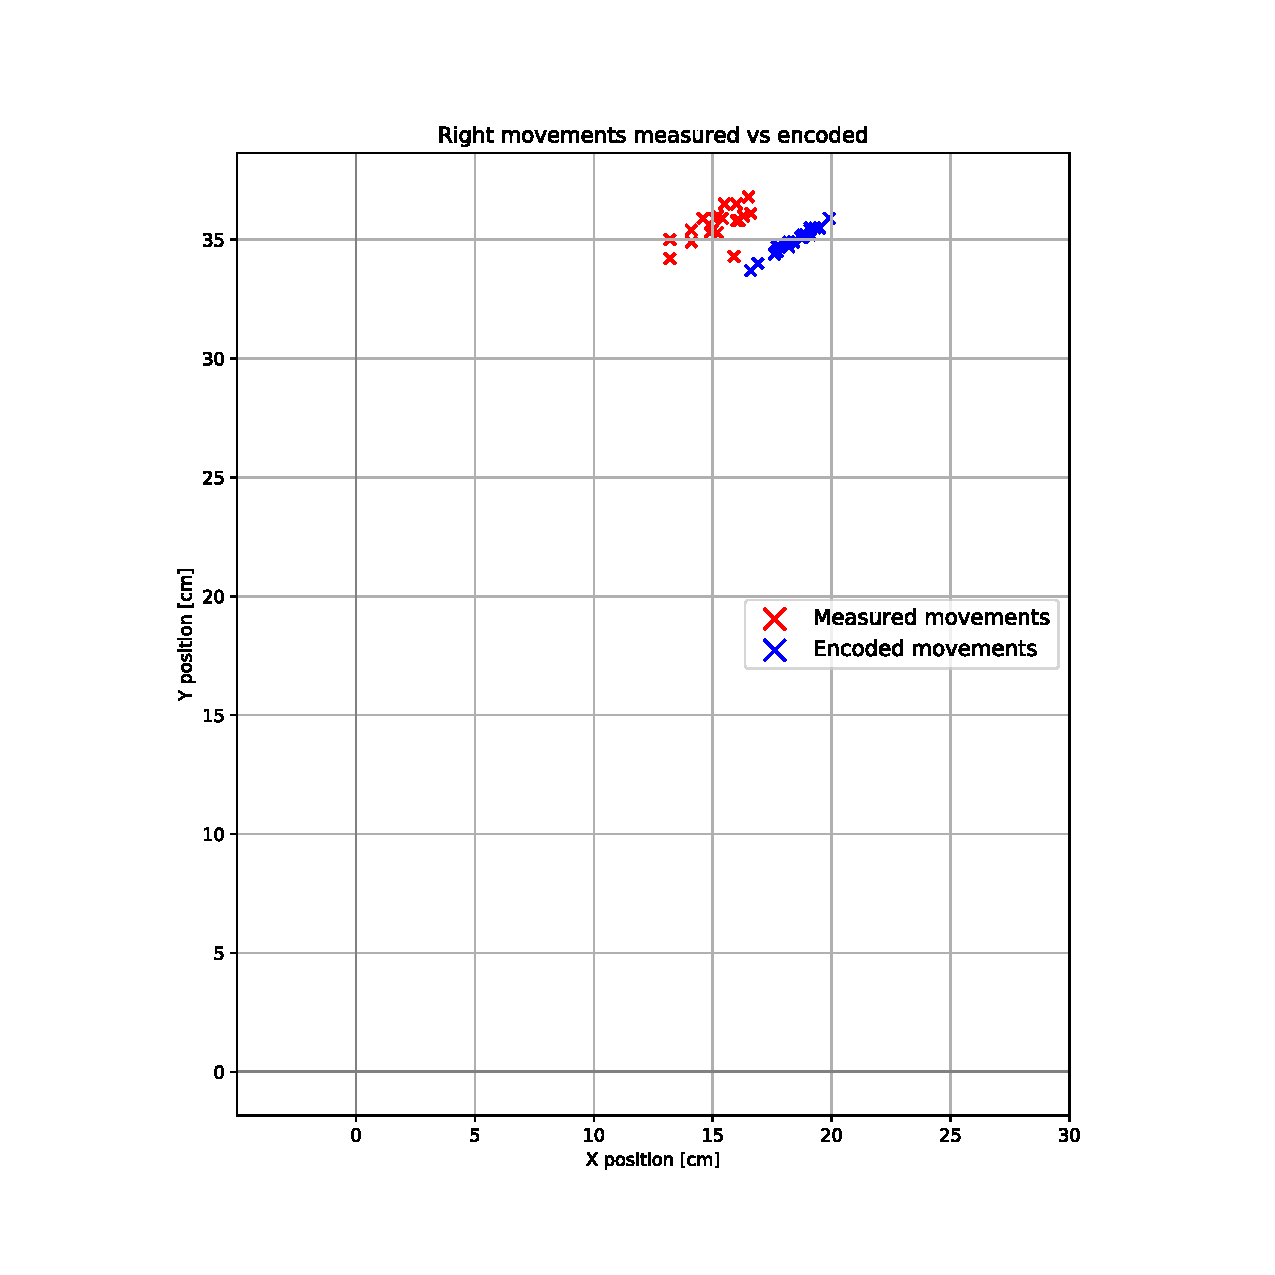
\includegraphics[page={1}, scale=.50]{images/pdf/right_movements_measured_and_encoded.pdf}
            \caption{Visualising the manually measured right poses and encoder logs}
            \label{fig:encoder-3}
    \end{figure}

    
        \begin{figure}[!ht] 
            \centering 
            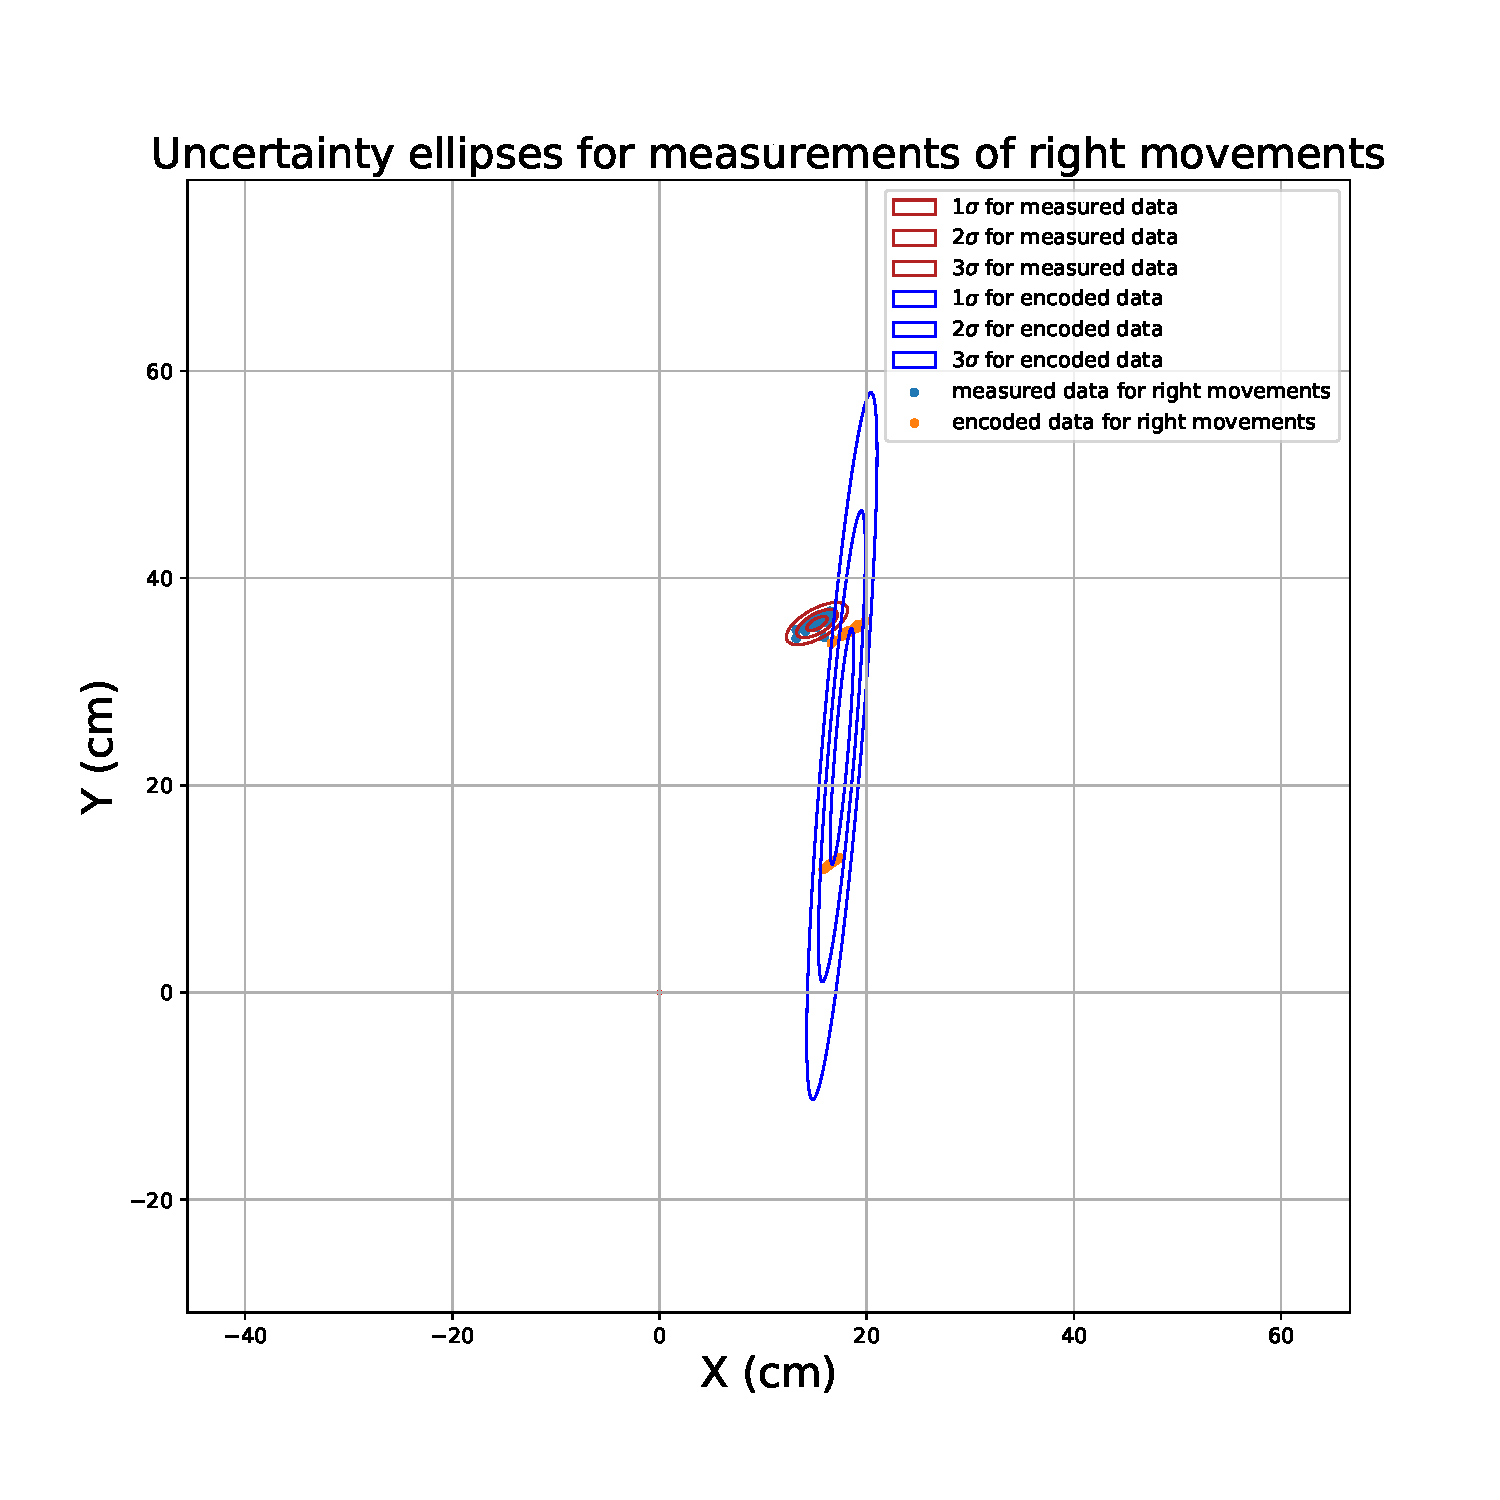
\includegraphics[page={1}, scale=.30]{images/pdf/ellipses_right_measured_vs_all_encoded.pdf}
            \caption{Overview of the encoder error}
            \label{fig:encoder-4}
    \end{figure}
    
    \begin{figure}[!ht] 
            \centering 
            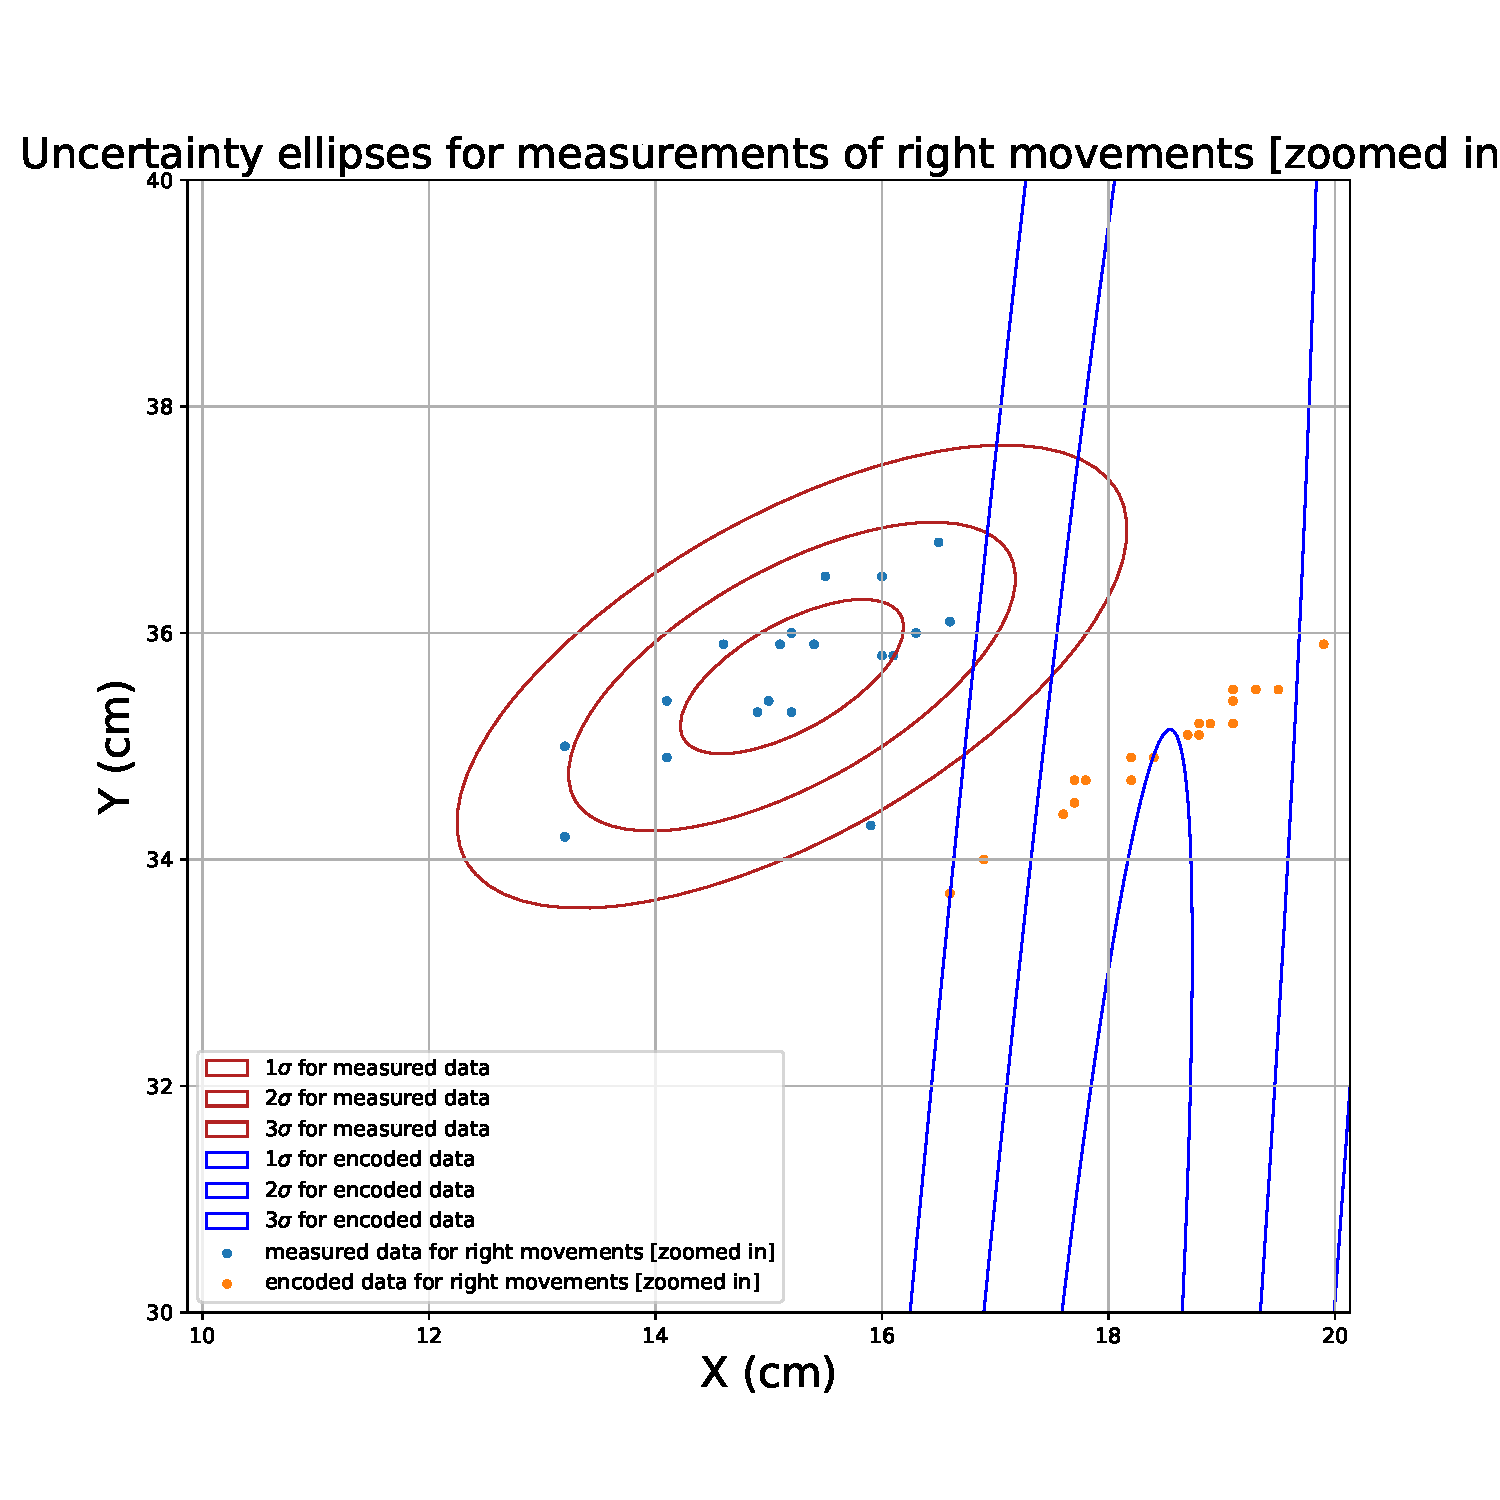
\includegraphics[page={1}, scale=.30]{images/pdf/ellipses_right_measured_vs_all_encoded_zoomed_in.pdf}
            \caption{Zoomed in view of the encoder error}
            \label{fig:encoder-5}
    \end{figure}
    
        
      \begin{figure}[!ht] 
            \centering 
            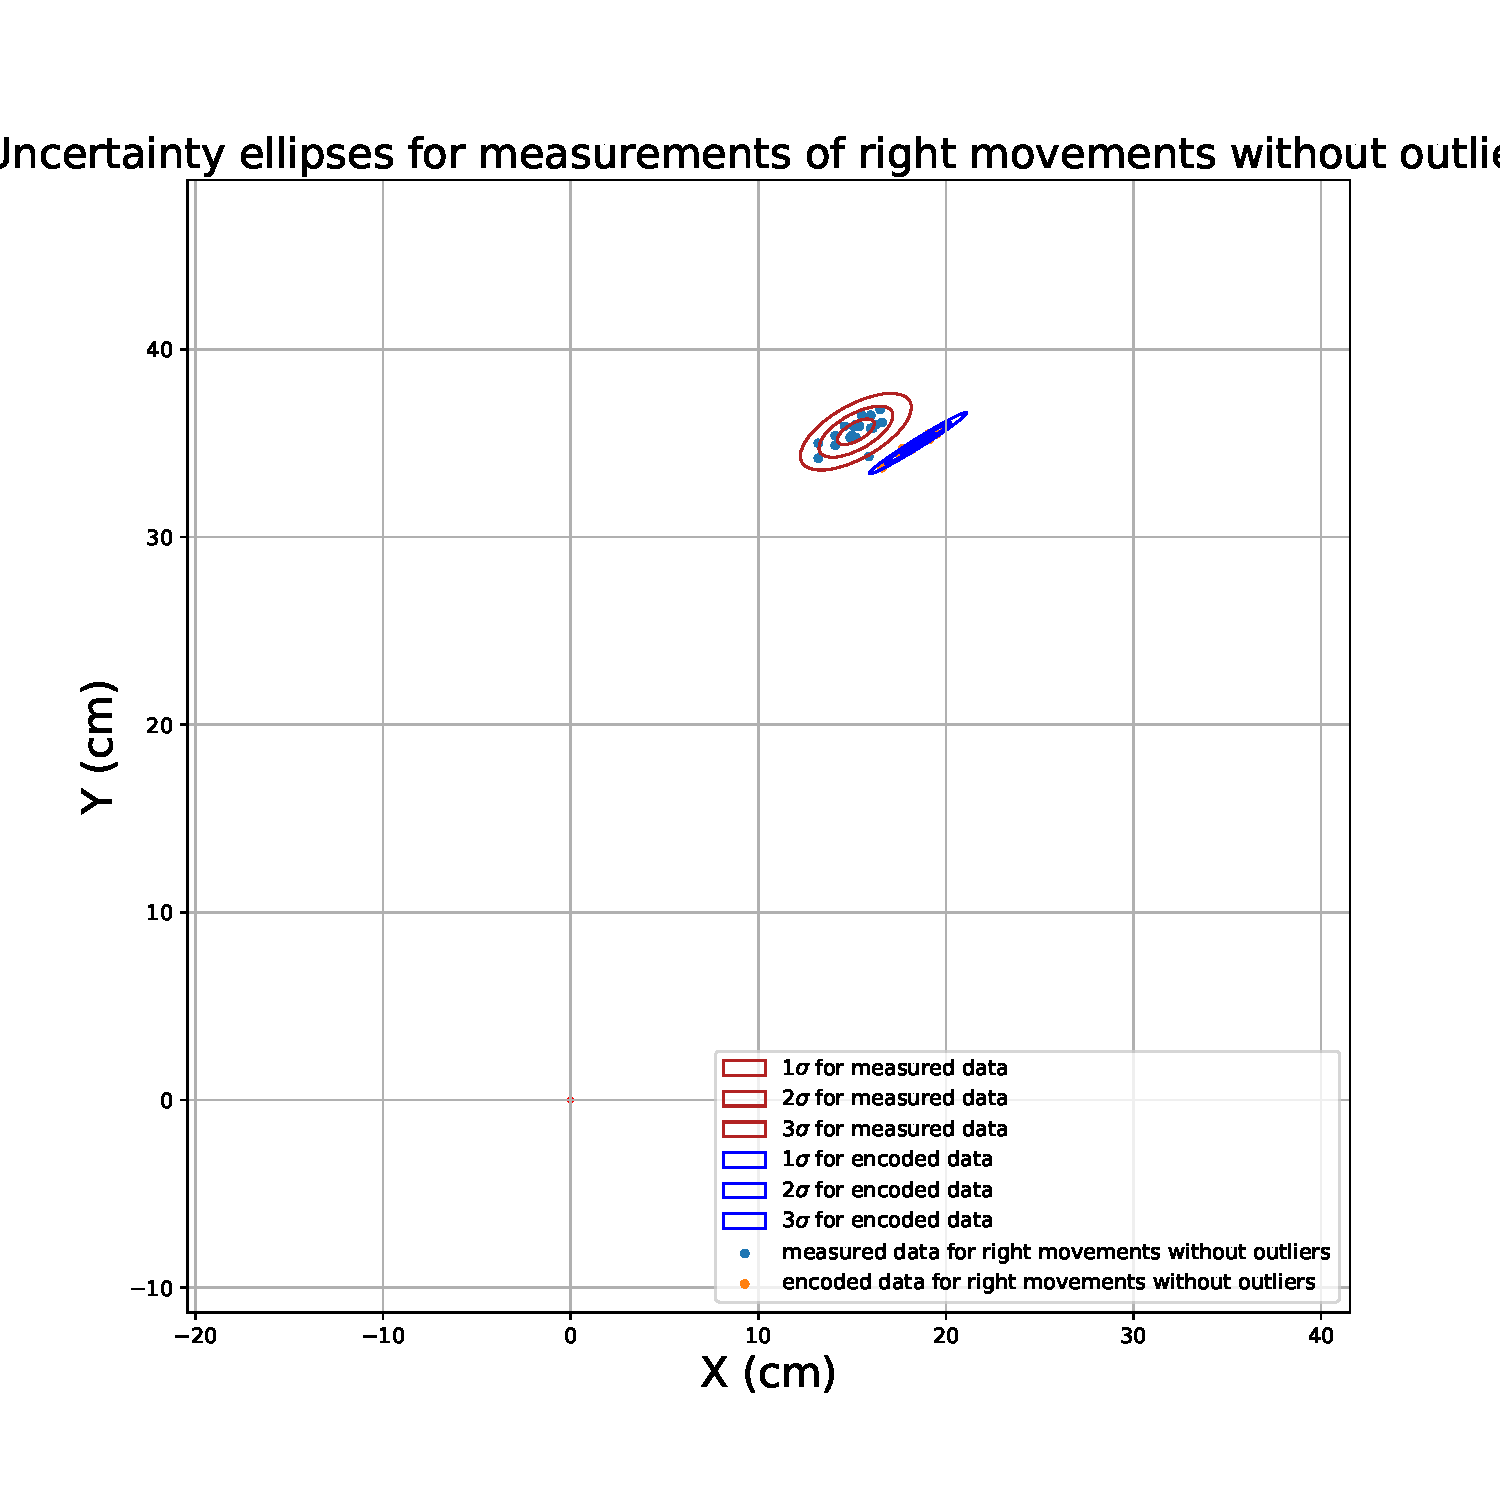
\includegraphics[page={1}, scale=.30]{images/pdf/ellipses_right_measured_vs_good_encoded.pdf}
            \caption{Overview of the encoder error without outliers}
            \label{fig:encoder-6}
    \end{figure}

          \begin{figure}[!ht] 
            \centering 
            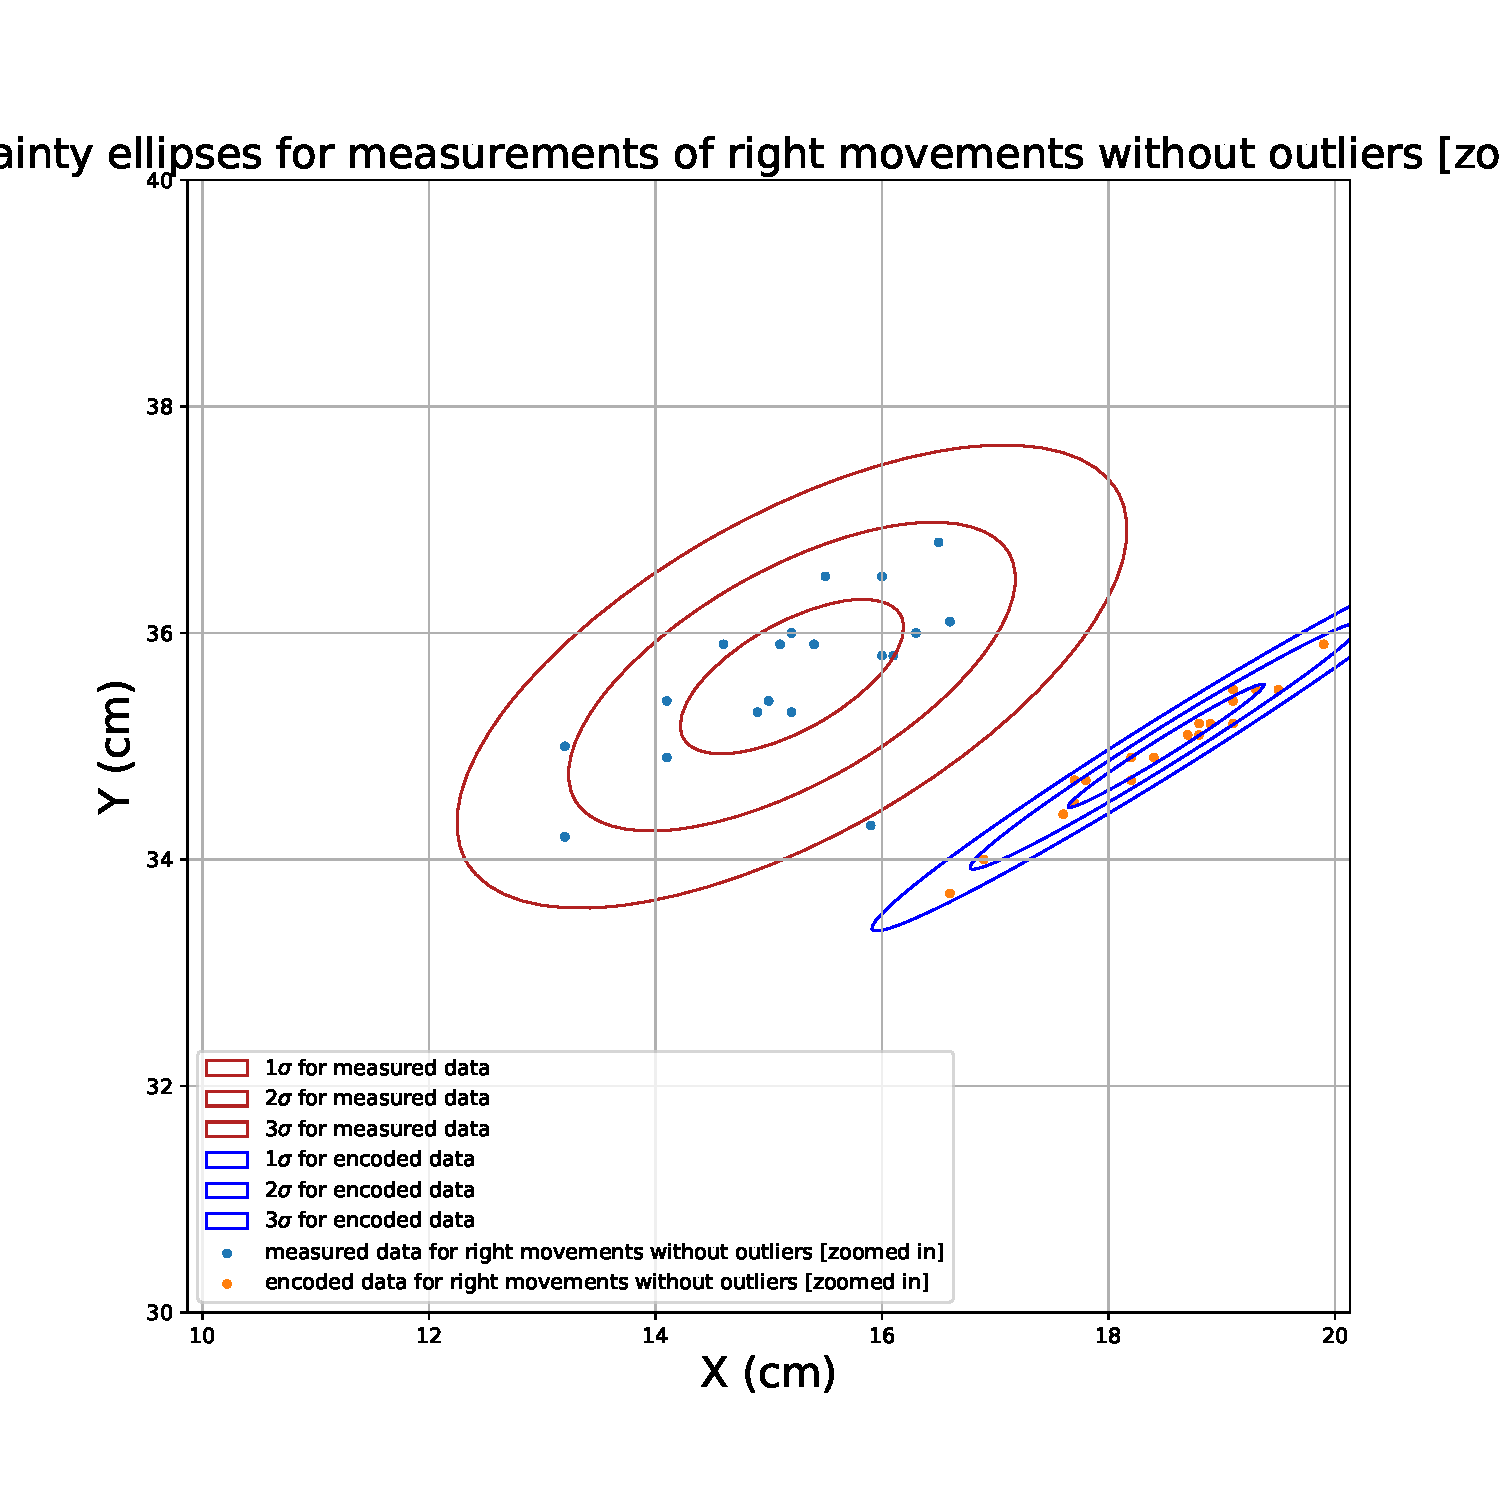
\includegraphics[page={1}, scale=.30]{images/pdf/ellipses_right_measured_vs_good_encoded_zoomed_in.pdf}
            \caption{Zoomed in view  of the encoder error without outliers}
            \label{fig:encoder-7}
    \end{figure}
    
    
    
    
    
    


    
\end{document}
